\documentclass[%
  aspectratio=169,
  9pt,
%   t,
  USenglish,
%english,
%   dark,
  light,
  mathserif,
%   serif, 
  professionalfont,
%  handout,
%  affiliationinhead,
  affiliationintitlepagehead,
  titlegraphic,
  %% The following options would violate the CD rules!
   affiliation,
%   uselogos,
  % navigationbar,
  %progressbar,
%   seprules,
%   titleinhead,
]{beamer}

%
%\usepackage{tikz}
%\usepackage{pgfplots}
%\usepgfplotslibrary{groupplots}



\usepackage{times}
\usepackage{epsfig}
\usepackage{graphicx}
\usepackage{amsmath}
\usepackage{amssymb}
\usepackage[utf8]{inputenc}
\usepackage{booktabs}
\setlength{\tabcolsep}{5pt}
\usepackage{subcaption}

\usepackage{appendix}
\usepackage{tummath}
\usepackage{tumtensors} % experimental
\usepackage{tumcolors}

\usepackage{pgfmath}
\newcommand\randmin{}
\newcommand\randmax{}
\newcommand\randmultof{}
\newcommand\setrand[4]%
{\def\randmin{#1}%
	\def\randmax{#2}%
	\def\randmultof{#3}%
	\pgfmathsetseed{#4}%
}
\newcommand\nextrand
{\pgfmathparse{int(int((rnd*(\randmax-\randmin+1)+\randmin)/\randmultof)*\randmultof)}%
	\xdef\thisrand{\pgfmathresult}%
}

% Include other packages here, before hyperref.

% If you comment hyperref and then uncomment it, you should delete
% egpaper.aux before re-running latex.  (Or just hit 'q' on the first latex
% run, let it finish, and you should be clear).
%\usepackage[breaklinks=true,bookmarks=false]{hyperref}


\usepackage[capitalize]{cleveref}
\usepackage[square,sort,comma,numbers]{natbib}

%% this hack seems to be nececessary due to incompatibilities of cvpr template and tikz... -> https://tex.stackexchange.com/questions/398223/tikz-gives-error-command-everyshipouthook-already-defined
\makeatletter
\@namedef{ver@everyshi.sty}{}
\makeatother
%% hackend

%{r\tikzsetnextfilenameawinput}

\newcommand{\rawtimeseries}[1]{

\begin{tikzpicture}[baseline=-2em, inner sep=0]

	\begin{axis}[
		thin,
		width=6cm,
		hide axis,
		height=3cm,
		ymin=0, ymax=1.4,
		no marks,  
		draw opacity=.8,
		smooth=0.01
	]
		 
	\addplot[b1color] table [x=t, y=B1, col sep=comma, forget plot] {images/example/#1};
	\addplot[b9color] table [x=t, y=B9, col sep=comma, forget plot] {images/example/#1};
	\addplot[b10color] table [x=t, y=B10, col sep=comma] {images/example/input.csv};
	
	\addplot[b11color] table [x=t, y=B11, col sep=comma, forget plot] {images/example/#1};
	\addplot[b12color] table [x=t, y=B12, col sep=comma] {images/example/#1};
	
	\addplot[b5color] table [x=t, y=B5, col sep=comma, forget plot] {images/example/#1};
	\addplot[b6color] table [x=t, y=B6, col sep=comma, forget plot] {images/example/#1};
	\addplot[b7color] table [x=t, y=B7, col sep=comma, forget plot] {images/example/#1};
	\addplot[b8color] table [x=t, y=B8, col sep=comma, forget plot] {images/example/#1};
	\addplot[b8Acolor] table [x=t, y=B8A, col sep=comma] {images/example/#1};
		
	\addplot[b2color] table [x=t, y=B2, col sep=comma, forget plot] {images/example/#1};
	\addplot[b3color] table [x=t, y=B3, col sep=comma, forget plot] {images/example/#1};
	\addplot[b4color] table [x=t, y=B4, col sep=comma] {images/example/#1};

	\end{axis}
	
\end{tikzpicture}
	
}

\usepackage{tikz}
\usepackage{pgfplots}
\usetikzlibrary{positioning, calc,arrows,arrows.meta, fit}
%\usetikzlibrary{arrows.meta,calc,decorations.markings,math,arrows.meta}
\usepgfplotslibrary{groupplots}
\usepgfplotslibrary{fillbetween}
\usepgfplotslibrary{statistics} % provides boxplots
\usepackage{xfrac}

\newcommand{\tp}{tp}
\newcommand{\tn}{tn}
\newcommand{\fp}{fp}
\newcommand{\fn}{fn}


\usepackage{tumcolors}
\usepackage{tummath}
\newcommand{\yhat}{\hat{\V{y}}}
\newcommand{\ycorrect}{\hat{y}^+}
\newcommand{\thetadelta}{\V{\Theta}_\delta}
\newcommand{\biasdelta}{b_\delta}
\newcommand{\biasclass}{\V{b}_\text{c}}
\newcommand{\thetaclass}{\V{\Theta}_\text{c}}
\newcommand{\thetafeat}{\V{\Theta}_\text{feat}}
\newcommand{\fclass}{f_\text{c}}
\newcommand{\fdelta}{f_\delta}
\newcommand{\ffeat}{f_\text{feat}}
\newcommand{\f}{f}

\newcommand{\rvtime}{T_c} 
\newcommand{\xuptot}{\M{X}_{\rightarrow t}} 
\newcommand{\deltauptot}{\delta_{\rightarrow t}} 
\newcommand{\tstop}{\ensuremath{t_\text{stop}}}
\newcommand{\meantstop}{\ensuremath{\bar{t}_\text{stop}}}
\usepackage[super]{nth}
\usepackage{mathtools}

\definecolor{evalcolor}{HTML}{3F3F3F}
\definecolor{traincolor}{HTML}{B98951}
\definecolor{validcolor}{HTML}{3F4BBE}

\colorlet{colortrain}{tumblue}
\colorlet{colorinfer}{tumblack}

\colorlet{earlinesscolor}{tumblue}
\colorlet{accuracycolor}{tumorange}

\colorlet{stdcolor}{tumbluelight}
\colorlet{mediancolor}{tumorange}
\colorlet{meancolor}{tumblue}

%\colorlet{b1color}{tumdiagramaubergine}
%\colorlet{b2color}{tumdiagramnavyblue}
%\colorlet{b3color}{tumdiagramturquoise}
%\colorlet{b4color}{tumdiagramgreen}
%\colorlet{b5color}{tumdiagramlimegreen}
%\colorlet{b6color}{tumdiagramyellow}
%\colorlet{b7color}{tumdiagramsand}
%\colorlet{b8color}{tumdiagramredorange}
%\colorlet{b8Acolor}{tumdiagramred}
%\colorlet{b9color}{tumblack}
%\colorlet{b10color}{tumblue}
%\colorlet{b11color}{tumdiagramdarkred}
%\colorlet{b12color}{tumorange}

% atmospheric bands
\colorlet{b1color}{tumblack}%tumdiagramaubergine
\colorlet{b9color}{tumblack}%tumblack
\colorlet{b10color}{tumblack}%tumblue

%visisble bands
\colorlet{b2color}{tumblue}%tumdiagramnavyblue
\colorlet{b3color}{tumblue}%tumdiagramturquoise
\colorlet{b4color}{tumblue}%tumdiagramgreen

% near infrared bands
\colorlet{b5color}{tumred}%tumdiagramlimegreen
\colorlet{b6color}{tumred}%tumdiagramyellow
\colorlet{b7color}{tumred}%tumdiagramsand
\colorlet{b8color}{tumred}%tumdiagramredorange
\colorlet{b8Acolor}{tumred}%tumdiagramred

% SWIR bands
\colorlet{b11color}{tumgreen}%tumdiagramdarkred
\colorlet{b12color}{tumgreen}%tumorange

\colorlet{epsilon0color}{tumorange}
\colorlet{epsilon1color}{tumblue}
\colorlet{epsilon10color}{tumblack}

\colorlet{meadowcolor}{tumbluemedium}
\colorlet{wbarleycolor}{tumbluedark}
\colorlet{corncolor}{tumorange}
\colorlet{wheatcolor}{tumgreen}
\colorlet{sbarleycolor}{tumred}
\colorlet{clovercolor}{tumturquoise}
\colorlet{triticalecolor}{tumsand}

\tikzstyle{rnn}=[draw,circle, inner sep=.1em]
\tikzstyle{norm}=[rounded corners,draw]
\tikzstyle{annot}=[rounded corners, fill=tumblue!20]
\tikzstyle{infer}=[-stealth, shorten >=.0em, shorten <=.0em, colorinfer]
\tikzstyle{loss}=[fill=tumblue!10, rounded corners, font=\small]
\tikzstyle{grad}=[colortrain]

\newcommand{\ptoffset}{\varepsilon}

\tikzstyle{test} = [thick]
\tikzstyle{train} = [thin, dotted]

\usepackage[inline]{enumitem}
\setenumerate{label=(\roman*),itemsep=3pt,topsep=3pt}

\setlength{\belowcaptionskip}{-10pt}
%\usepackage{titlesec}
%\titlespacing{\section}{0pt}{10pt}{3pt}

\usetikzlibrary{external}
\tikzexternalize[prefix=tikz/]
%\tikzexternalize
\tikzexternaldisable

\usepackage[eulergreek]{sansmath}
\pgfplotsset{
	y tick label style={/pgf/number format/.cd,%
		scaled y ticks = false,
		set thousands separator={},
		fixed},
	x tick label style={/pgf/number format/.cd,%
		scaled x ticks = false,
		set decimal separator={,},
		fixed},
	tick label style = {font=\sansmath\sffamily},
	every axis label = {
		font=\sansmath\sffamily},
	every axis/.append style={
		axis lines=left, 
		enlargelimits, 
		thick},
	legend style = {font=\sansmath\sffamily, draw=none, rounded corners, fill opacity=.5, text opacity=1},
	label style = {font=\sansmath\sffamily},
	grid style={line width=.1pt, draw=gray!10},
	major grid style={line width=.2pt,draw=tumgraylight},
}

%\let\tempone\itemize
%\let\temptwo\enditemize
%\renewenvironment{itemize}{\tempone\addtolength{\itemsep}{-.5\baselineskip}}{\temptwo}

\tikzstyle{circ} = [circle, draw=white, fill=tumblue, inner sep=1pt]
\newcommand{\fcn}{
	\begin{tikzpicture}[scale=0.2, rotate=0, baseline=-.25em, inner sep=1pt]
	\node[circ](a0) at (0,-1){};
	\node[circ](a1) at (0,0){};
	\node[circ](a2) at (0,1){};
	
	\node[circ](b0) at (1,-0.5){};
	\node[circ](b1) at (1,0.5){};
	
	\draw[-] (a0) -- (b0);
	\draw[-] (a1) -- (b0);
	\draw[-] (a2) -- (b0);
	
	\draw[-] (a0) -- (b1);
	\draw[-] (a1) -- (b1);
	\draw[-] (a2) -- (b1);
	
	\end{tikzpicture}
}


\newcommand{\earth}{
	\begin{tikzpicture}[baseline=-.25em, inner sep=0]
	\node{
\includegraphics[width=8mm]{images/icons/earth}};
	\end{tikzpicture}
}

\newcommand{\sat}{
	\begin{tikzpicture}[baseline=-.25em, inner sep=0]
	\node[rotate=270,anchor=center]{
\includegraphics[width=8mm]{images/icons/sat2}};
	\end{tikzpicture}
}

\newcommand{\hidden}[1]{
	\begin{tikzpicture}[scale=.1, baseline=-.25em]	
	%\draw[step=1.0,black,thin] (0,0) grid (#1,1);
	\foreach \i in {1,...,#1}{
		\node[circle, draw=white, fill=tumbluelight, inner sep=1pt] at (\i,0){};
	}
	\end{tikzpicture}
}

\newcommand{\drawvector}[1]{
	\begin{tikzpicture}[scale=.1, baseline=-.25em]	
	%\draw[step=1.0,black,thin] (0,0) grid (#1,1);
	\foreach \i in {1,...,#1}{
		\node[circ] at (\i,0){};
	}
	\end{tikzpicture}
}
\tikzstyle{proba} = [circle, draw=tumgray, inner sep=2.5pt, fill=tumorange]
\newcommand{\drawprobas}[5]{
	\begin{tikzpicture}[scale=.3, baseline=-.25em]	

	\node[proba, fill=tumblue!#1] at (0,-2){};
	\node[proba, fill=tumblue!#2] at (0,-1){};
	\node[proba, fill=tumblue!#3] at (0,-0){};
	\node[proba, fill=tumblue!#4] at (0,1){};
	\node[proba, fill=tumblue!#5] at (0,2){};
	\end{tikzpicture}
}

\newcommand{\vegetationsmodell}{
	\begin{tikzpicture}[scale=0.5, rotate=0, baseline=-.25em]
	\node[proba](a0) at (0,-1){};
	\node[proba](a1) at (0,0){};
	\node[proba](a2) at (0,1){};
	
	\node[proba](b0) at (1,-0.5){};
	\node[proba](b1) at (1,0.5){};
	
	\draw[-] (a0) -- (b0);
	\draw[-] (a1) -- (b0);
	\draw[-] (a2) -- (b0);
	
	\draw[-] (a0) -- (b1);
	\draw[-] (a1) -- (b1);
	\draw[-] (a2) -- (b1);
	
	\node[fit=(a0)(a2)(b1),draw,rounded corners](node name){};
	
	\end{tikzpicture}
}
\usetheme{TUM}

%{r\tikzsetnextfilenameawinput}

\newcommand{\rawtimeseries}[1]{

\begin{tikzpicture}[baseline=-2em, inner sep=0]

	\begin{axis}[
		thin,
		width=6cm,
		hide axis,
		height=3cm,
		ymin=0, ymax=1.4,
		no marks,  
		draw opacity=.8,
		smooth=0.01
	]
		 
	\addplot[b1color] table [x=t, y=B1, col sep=comma, forget plot] {images/example/#1};
	\addplot[b9color] table [x=t, y=B9, col sep=comma, forget plot] {images/example/#1};
	\addplot[b10color] table [x=t, y=B10, col sep=comma] {images/example/input.csv};
	
	\addplot[b11color] table [x=t, y=B11, col sep=comma, forget plot] {images/example/#1};
	\addplot[b12color] table [x=t, y=B12, col sep=comma] {images/example/#1};
	
	\addplot[b5color] table [x=t, y=B5, col sep=comma, forget plot] {images/example/#1};
	\addplot[b6color] table [x=t, y=B6, col sep=comma, forget plot] {images/example/#1};
	\addplot[b7color] table [x=t, y=B7, col sep=comma, forget plot] {images/example/#1};
	\addplot[b8color] table [x=t, y=B8, col sep=comma, forget plot] {images/example/#1};
	\addplot[b8Acolor] table [x=t, y=B8A, col sep=comma] {images/example/#1};
		
	\addplot[b2color] table [x=t, y=B2, col sep=comma, forget plot] {images/example/#1};
	\addplot[b3color] table [x=t, y=B3, col sep=comma, forget plot] {images/example/#1};
	\addplot[b4color] table [x=t, y=B4, col sep=comma] {images/example/#1};

	\end{axis}
	
\end{tikzpicture}
	
}

%%%%%%%%%%%%%%%%%%%%%%%%%%%%%%%%%%%%%%%%%%%%%%%%%%%%%%%%%%%%%%%%%%%%%%%%%%%%%%%%%%%%%%%

%Convolutional-Recurrent Networks for Multi-temporal Classification
\title{Cloud-Robust Classification of Remote Sensing Time Series}
%\subtitle{NeurIPS 2018 Workshop on Spatiotemporal Modeling and Decision-making}
\subtitle{$\Phi$-week 2019}
\author[M. Rußwurm, M. Körner]{Marc Rußwurm, Marco Körner}
\institute[TUM]{Technical University of Munich\\Chair of Remote Sensing Technology\\Computer Vision Research Group\\\url{www.lmf.bgu.tum.de/vision}}

\date{13th September 2019, ESA ESRIN, Frascati, Italy}

\begin{document}

\begin{frame}[t]
  \titlepage
\end{frame}


{{\setbeamertemplate{background canvas}{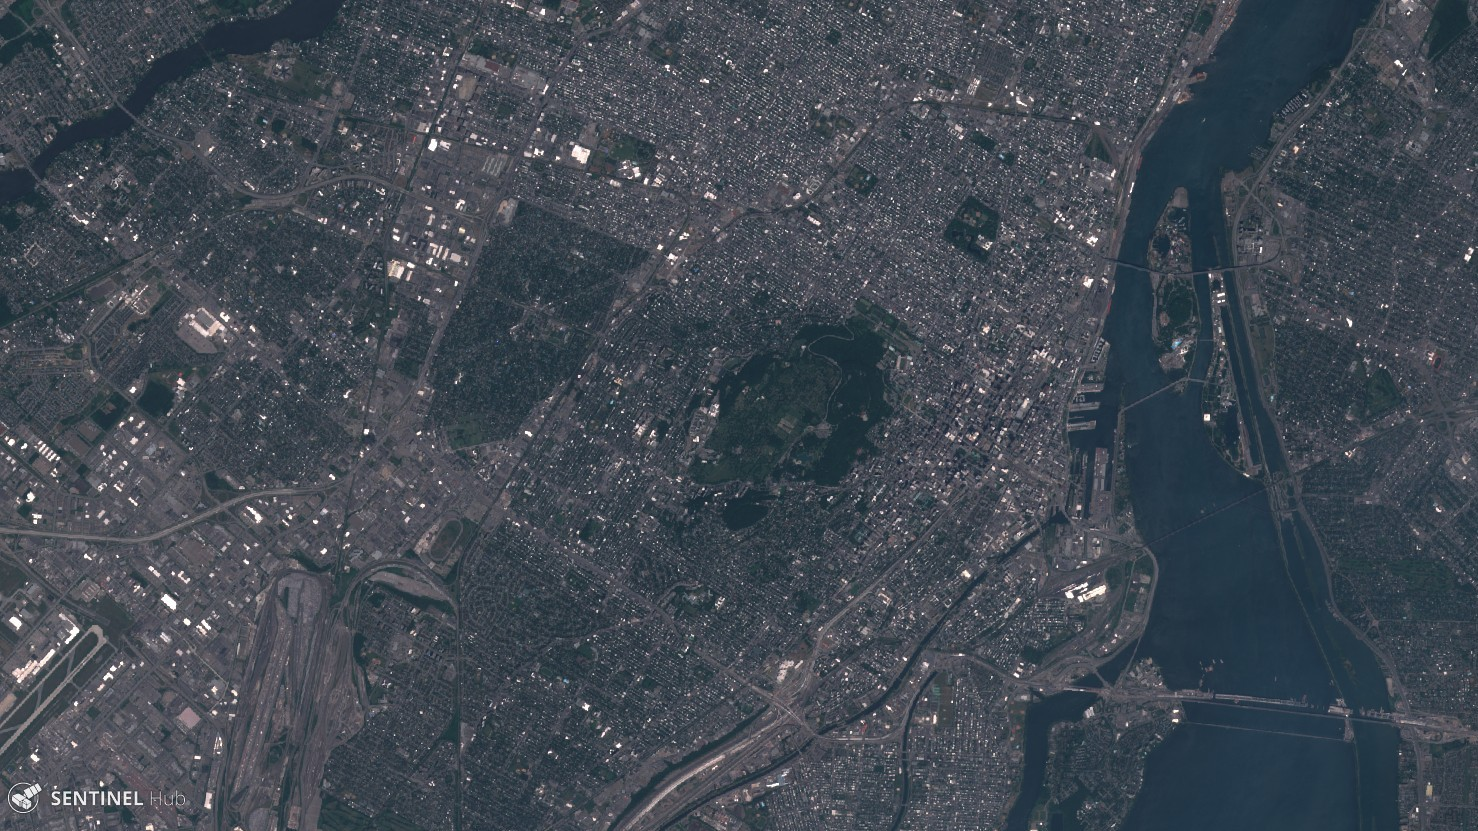
\includegraphics[width=\paperwidth]{images/cloudfree}}
\begin{frame}[plain]
%\frametitle{When we think of satellite images we picture this}
%%\centering\includegraphics[width=.75\textwidth]{images/montreal_satellite}
%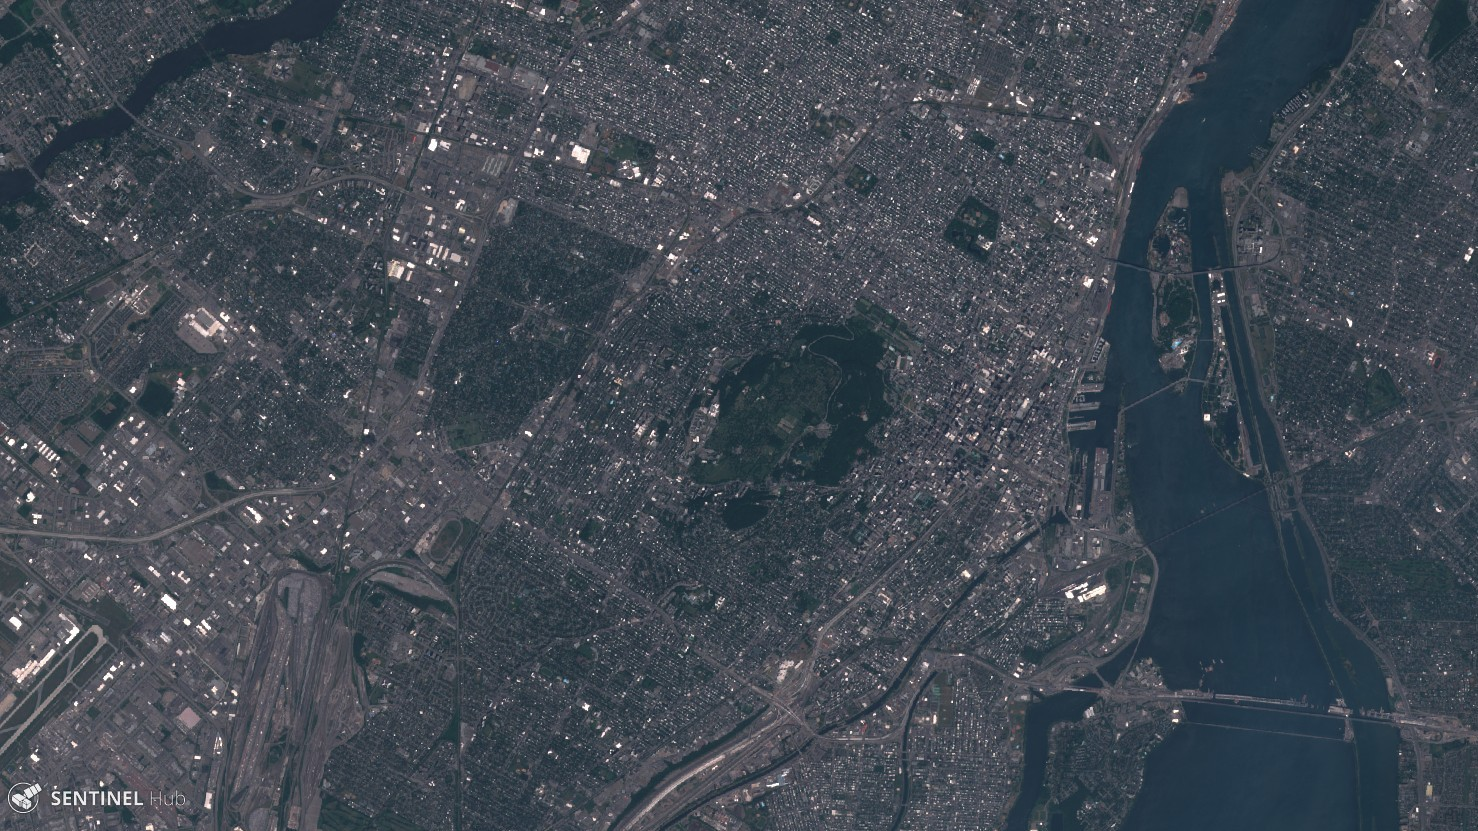
\includegraphics[width=\textwidth]{images/cloudfree}
\end{frame}
}

{\setbeamertemplate{background canvas}{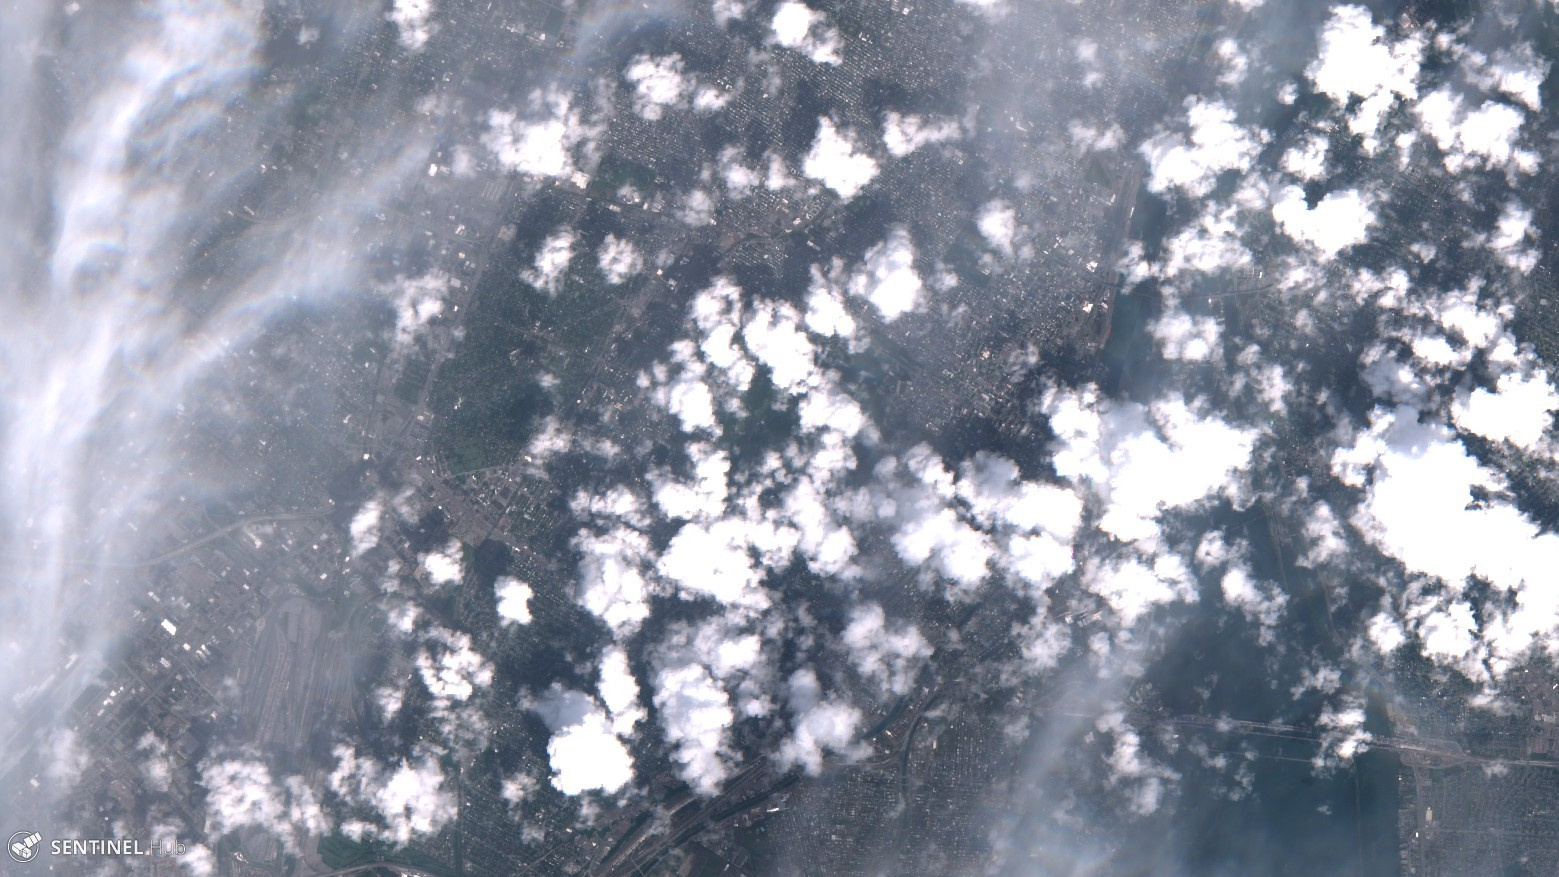
\includegraphics[width=\paperwidth]{images/clouds}}
	\begin{frame}[plain]
%		\frametitle{... however, ususally }
			
		
	%		\includegraphics[width=\textwidth]{images/cloud_airplane}
			
	\end{frame}
	
}

{\setbeamercolor{background canvas}{bg=tumbluedark}
	\begin{frame}[plain]
	
	\vspace{8em}
	\begin{center}
		\Huge\color{tumwhite}
		How should we deal with $
\includegraphics[width=2em]{images/icons/cloud2}^\ast$?
	\end{center}\color{white}
	\vspace{2em}
	\raggedleft \Large$^\ast$ ...and other noise in the data
	
	\vfill
	\vspace{6em}
	\raggedleft{\small \color{tumgray}
	Icons made by Smashicons from www.flaticon.com
	}
\end{frame}
}tumorange


\begin{frame}<presentation:1>
\frametitle{Cloud coverage}
\centering

\def\imagewidth{1.5cm}


\visible<1>{\includegraphics[width=\imagewidth]{images/activations/16494/x/x-0.png}}
\visible<1>{\includegraphics[width=\imagewidth]{images/activations/16494/x/x-1.png}}
\visible<1>{\includegraphics[width=\imagewidth]{images/activations/16494/x/x-2.png}}
\visible<1>{\includegraphics[width=\imagewidth]{images/activations/16494/x/x-3.png}}
\visible<1>{\includegraphics[width=\imagewidth]{images/activations/16494/x/x-4.png}}
\visible<1,2>{\includegraphics[width=\imagewidth]{images/activations/16494/x/x-5.png}}
\visible<1>{\includegraphics[width=\imagewidth]{images/activations/16494/x/x-6.png}}
\visible<1>{\includegraphics[width=\imagewidth]{images/activations/16494/x/x-7.png}}
\visible<1,2>{\includegraphics[width=\imagewidth]{images/activations/16494/x/x-8.png}}
\visible<1>{\includegraphics[width=\imagewidth]{images/activations/16494/x/x-9.png}}
\visible<1>{\includegraphics[width=\imagewidth]{images/activations/16494/x/x-10.png}}
\visible<1>{\includegraphics[width=\imagewidth]{images/activations/16494/x/x-11.png}}
\visible<1,2>{\includegraphics[width=\imagewidth]{images/activations/16494/x/x-12.png}}
\visible<1,2>{\includegraphics[width=\imagewidth]{images/activations/16494/x/x-13.png}}
\visible<1,2>{\includegraphics[width=\imagewidth]{images/activations/16494/x/x-14.png}}
\visible<1,2>{\includegraphics[width=\imagewidth]{images/activations/16494/x/x-15.png}}
\visible<1,2>{\includegraphics[width=\imagewidth]{images/activations/16494/x/x-16.png}}
\visible<1>{\includegraphics[width=\imagewidth]{images/activations/16494/x/x-18.png}}
\visible<1>{\includegraphics[width=\imagewidth]{images/activations/16494/x/x-19.png}}
\visible<1,2>{\includegraphics[width=\imagewidth]{images/activations/16494/x/x-20.png}}
\visible<1,2>{\includegraphics[width=\imagewidth]{images/activations/16494/x/x-21.png}}
\visible<1>{\includegraphics[width=\imagewidth]{images/activations/16494/x/x-22.png}}
\visible<1>{\includegraphics[width=\imagewidth]{images/activations/16494/x/x-23.png}}
\visible<1>{\includegraphics[width=\imagewidth]{images/activations/16494/x/x-24.png}}
\visible<1>{\includegraphics[width=\imagewidth]{images/activations/16494/x/x-25.png}}
\visible<1>{\includegraphics[width=\imagewidth]{images/activations/16494/x/x-26.png}}
\visible<1,2>{\includegraphics[width=\imagewidth]{images/activations/16494/x/x-27.png}}
\visible<1>{\includegraphics[width=\imagewidth]{images/activations/16494/x/x-28.png}}
\visible<1,2>{\includegraphics[width=\imagewidth]{images/activations/16494/x/x-29.png}}
\visible<1>{\includegraphics[width=\imagewidth]{images/activations/16494/x/x-30.png}}
\visible<1>{\includegraphics[width=\imagewidth]{images/activations/16494/x/x-31.png}}
\visible<1,2>{\includegraphics[width=\imagewidth]{images/activations/16494/x/x-32.png}}
\visible<1>{\includegraphics[width=\imagewidth]{images/activations/16494/x/x-33.png}}
%	
\end{frame}

\newcommand{\xtvector}{
	\begin{tikzpicture}[baseline=-1.9em,yscale=-5]
		\node[draw=tumgraylight, circle, fill=b2color, text=white, text opacity=1, font=\small, inner sep=.1em](d) at (0,0){};
		\node[draw=tumgraylight, circle, fill=b3color, text=white, text opacity=1, font=\small, inner sep=.1em](d) at (0,1){};
		\node[draw=tumgraylight, circle, fill=b4color, text=white, text opacity=1, font=\small, inner sep=.1em](d) at (0,2){};
		\node[draw=tumgraylight, circle, fill=b5color, text=white, text opacity=1, font=\small, inner sep=.1em](d) at (0,3){};
		\node[draw=tumgraylight, circle, fill=b6color, text=white, text opacity=1, font=\small, inner sep=.1em](d) at (0,4){};
		\node[draw=tumgraylight, circle, fill=b7color, text=white, text opacity=1, font=\small, inner sep=.1em](d) at (0,5){};
		\node[draw=tumgraylight, circle, fill=b8color, text=white, text opacity=1, font=\small, inner sep=.1em](d) at (0,6){};
		\node[draw=tumgraylight, circle, fill=b8Acolor, text=white, text opacity=1, font=\small, inner sep=.1em](d) at (0,7){};
		\node[draw=tumgraylight, circle, fill=b11color, text=white, text opacity=1, font=\small, inner sep=.1em](d) at (0,8){};
		\node[draw=tumgraylight, circle, fill=b12color, text=white, text opacity=1, font=\small, inner sep=.1em](d) at (0,9){};
	\end{tikzpicture}
}



\begin{frame}
	\frametitle{Looking at single pixels}
	\framesubtitle{Sentinel 2 (raw)}
	
	
	
	
	
	\begin{tikzpicture}[baseline=-2em, inner sep=0]
		
		\begin{axis}[
		width=\textwidth,
	%	hide axis,
		height=5.5cm,
		ymin=0, ymax=1.2,
		%no marks,  
		draw opacity=.8,
		smooth=0.001,
		legend style={at={(1,1.3)},line width=2pt, draw opacity=1},
		legend columns=5,
		ylabel={reflectance},
		xlabel={time $t$ {\small (January to December 2018)}}
		]
		
		
			\addplot[b2color, tsmark] table [x=t, y=B02, col sep=comma] {images/example/12-71456800_raw.csv};
			\addplot[b3color, tsmark] table [x=t, y=B03, col sep=comma] {images/example/12-71456800_raw.csv};
			\addplot[b4color, tsmark] table [x=t, y=B04, col sep=comma] {images/example/12-71456800_raw.csv};
			
			\only<2-3>{
				 \coordinate(c1) at (axis cs:15,1.1);
				 \coordinate(c2) at (axis cs:10,.8);
				 \coordinate(c3) at (axis cs:0,.6);
				 \coordinate(c4) at (axis cs:40,.6);
				 \coordinate(c5) at (axis cs:46,.6);
%				 \coordinate(c6) at (axis cs:0,.6);
				 
				 \coordinate(c8) at (axis cs:24,.9);
				 \coordinate(c9) at (axis cs:27,.8);
				 \coordinate(c7) at (axis cs:29,.9);
				 
				 
				 \node[inner sep=.5em](annotclouds) at (axis cs:32,1.2){clouds};
				 \draw[-stealth] (annotclouds) -- (c7);
				 \draw[-stealth] (annotclouds) -- (c8);
				 \draw[-stealth] (annotclouds) -- (c9);
				 \draw[-stealth] (annotclouds) -- (c4);
				 \draw[-stealth] (annotclouds) -- (c5);
				 \draw[-stealth] (annotclouds) -- (c1);
%				 \draw[-stealth] (annotclouds) -- (c6);
				 
			}
			\only<3-3>{
				
				\node[inner sep=.5em](annotground) at (axis cs:47,1.2){ground};
				\coordinate(g1) at (axis cs:4,.2);
				\coordinate(g2) at (axis cs:8,.2);
				\coordinate(g3) at (axis cs:13,.2);
				\coordinate(g4) at (axis cs:18,.2);
				\coordinate(g5) at (axis cs:23,.2);
				\coordinate(g6) at (axis cs:31,.2);
				\coordinate(g7) at (axis cs:35,.2);
				\coordinate(g8) at (axis cs:41,.2);
				\coordinate(g9) at (axis cs:47,.2);
				
%				\draw[-stealth] (annotground) -- (g1);
%				\draw[-stealth] (annotground) -- (g2);
%				\draw[-stealth] (annotground) -- (g3);
%				\draw[-stealth] (annotground) -- (g4);
%				\draw[-stealth] (annotground) -- (g5);
				\draw[-stealth] (annotground) -- (g6);
				\draw[-stealth] (annotground) -- (g7);
				\draw[-stealth] (annotground) -- (g8);
				\draw[-stealth] (annotground) -- (g9);
				
			}
			
			\only<1->{
			\addplot[b5color, tsmark] table [x=t, y=B05, col sep=comma] {images/example/12-71456800_raw.csv};
			\addplot[b6color, tsmark] table [x=t, y=B06, col sep=comma] {images/example/12-71456800_raw.csv};
			\addplot[b7color, tsmark] table [x=t, y=B07, col sep=comma] {images/example/12-71456800_raw.csv};
			\addplot[b8color, tsmark] table [x=t, y=B08, col sep=comma] {images/example/12-71456800_raw.csv};
			\addplot[b8Acolor, tsmark] table [x=t, y=B8A, col sep=comma] {images/example/12-71456800_raw.csv};
			
			\addplot[b11color, tsmark] table [x=t, y=B11, col sep=comma] {images/example/12-71456800_raw.csv};
			\addplot[b12color, tsmark] table [x=t, y=B12, col sep=comma] {images/example/12-71456800_raw.csv};
			}
		
			\only<1-3>
			\legend{B02 (blue),B03 (green),B04 (red),B05,B06,B07,B08,B8A,B11,B12}
			
		\end{axis}
		
	\end{tikzpicture}
	
\end{frame}


\begin{frame}
\frametitle{Introducing Notation}


\begin{tikzpicture}[baseline=-2em, inner sep=0]

\begin{axis}[
width=\textwidth,
%	hide axis,
height=5.5cm,
ymin=0, ymax=1.2,
%no marks,  
draw opacity=.8,
smooth=0.001,
legend style={at={(.65,1.1)},line width=2pt, draw opacity=1},
legend columns=3,
ylabel={reflectance},
xlabel={time $t$}
]

\addplot[b2color, tsmark, opacity=.6] table [x=t, y=B02, col sep=comma] {images/example/12-71456800_raw.csv};
\addplot[b3color, tsmark, opacity=.6] table [x=t, y=B03, col sep=comma] {images/example/12-71456800_raw.csv};
\addplot[b4color, tsmark, opacity=.6] table [x=t, y=B04, col sep=comma] {images/example/12-71456800_raw.csv};
\addplot[b5color, tsmark, opacity=.6] table [x=t, y=B05, col sep=comma] {images/example/12-71456800_raw.csv};
\addplot[b6color, tsmark, opacity=.6] table [x=t, y=B06, col sep=comma] {images/example/12-71456800_raw.csv};
\addplot[b7color, tsmark, opacity=.6] table [x=t, y=B07, col sep=comma] {images/example/12-71456800_raw.csv};
\addplot[b8color, tsmark, opacity=.6] table [x=t, y=B08, col sep=comma] {images/example/12-71456800_raw.csv};
\addplot[b8Acolor, tsmark, opacity=.6] table [x=t, y=B8A, col sep=comma] {images/example/12-71456800_raw.csv};
\addplot[b11color, tsmark, opacity=.6] table [x=t, y=B11, col sep=comma] {images/example/12-71456800_raw.csv};
\addplot[b12color, tsmark, opacity=.6] table [x=t, y=B12, col sep=comma] {images/example/12-71456800_raw.csv};

\node[draw=tumbluedark, rounded corners, inner sep=0, minimum width=.8em, minimum height=3em](xt) at (axis cs:32,0.22){};
\node[font=\Large] (annotxt) at (axis cs:38,1.05){$\V{x}_t = 
	\begin{pmatrix} \rho_\text{B02} \\ \vdots \\ \rho_\text{B12} \end{pmatrix} = 
	\left(\xtvector\right)$};
\draw[-stealth] (annotxt) -- (xt);

%
%\only<1>{
%	\legend{B02 (blue),B03 (green),B04 (red),B05,B06,B07,B08,B8A,B11,B12}
%}

\end{axis}

\end{tikzpicture}

\end{frame}

\begin{frame}
\frametitle{Introducing Notation}

\vspace{-2em}

\begin{tikzpicture}
\node[](X){$\left(
\begin{tikzpicture}[baseline=-4em,yscale=-.25, xscale=.4]
\foreach \x in {0,...,22}{
	\node[draw=tumgraylight, circle, fill=b2color, text=white, text opacity=1, font=\small, inner sep=.2em](d) at (\x,0){};
	\node[draw=tumgraylight, circle, fill=b3color, text=white, text opacity=1, font=\small, inner sep=.2em](d) at (\x,1){};
	\node[draw=tumgraylight, circle, fill=b4color, text=white, text opacity=1, font=\small, inner sep=.2em](d) at (\x,2){};
	\node[draw=tumgraylight, circle, fill=b5color, text=white, text opacity=1, font=\small, inner sep=.2em](d) at (\x,3){};
	\node[draw=tumgraylight, circle, fill=b6color, text=white, text opacity=1, font=\small, inner sep=.2em](d) at (\x,4){};
	\node[draw=tumgraylight, circle, fill=b7color, text=white, text opacity=1, font=\small, inner sep=.2em](d) at (\x,5){};
	\node[draw=tumgraylight, circle, fill=b8color, text=white, text opacity=1, font=\small, inner sep=.2em](d) at (\x,6){};
	\node[draw=tumgraylight, circle, fill=b8Acolor, text=white, text opacity=1, font=\small, inner sep=.2em](d) at (\x,7){};
	\node[draw=tumgraylight, circle, fill=b11color, text=white, text opacity=1, font=\small, inner sep=.2em](d) at (\x,8){};
	\node[draw=tumgraylight, circle, fill=b12color, text=white, text opacity=1, font=\small, inner sep=.2em](d) at (\x,9){};
}
\end{tikzpicture}\right) \Huge \in \mathbb{R}^{D \times T}$};

\node[draw, rounded corners, xshift=1.85em, minimum width=1em, minimum height=8.5em, label={[name=featurevector]above:$\V{x}_t$}] at (X){};

\node[left=.5em of X, font=\Huge](Xmatr){$\M{X} = $};


\node[above=4em of Xmatr, xshift=2em] (annotmatrix){Input Matrix};
\node[above=1em of featurevector] (annotfeat){feature vector at time $t$};

\draw[-stealth] (annotfeat) -- (featurevector);
\draw[-stealth] (annotmatrix) -- (Xmatr);

\node[below=5em of Xmatr, font=\Huge](yvect){$\V{y} = $};

\node[right=.1em of yvect](gt){$\begin{pmatrix}
	{y}_i\\ \vdots \\ {y}_C
	\end{pmatrix} = \left(\drawprobas{0}{0}{0}{100}{0}\right) \text{where}~y_i \in \{0,1\}$};

\node[right=1em of gt, font=\Huge](yvect2){$\yhat =$};
\node[right=.1em of yvect2](gt2){$\begin{pmatrix}
	\hat{y}_i\\ \vdots \\ \hat{y}_C
	\end{pmatrix} = \left(\drawprobas{10}{30}{10}{90}{10}\right) \text{where}~\hat{y}_i \in [0,1]$ and $C$ classes};

\node[below=2em of yvect, xshift=2em] (annoty){ground truth};

\node[below=2em of yvect2, xshift=2em] (annoty2){prediction};
\draw[-stealth] (annoty) -- (yvect);
\draw[-stealth] (annoty2) -- (yvect2);

%	\node[below right=of Xmatr] (annotmatrix){Input Matrix};
\end{tikzpicture}
\end{frame}

\begin{frame}
	\frametitle{Data Preprocessing}
%	
%	[format] in this presentation we have the special opportunity to to compare commercially pre-processed satellite imagery with raw imagery on crop type classification in Bavaria Germany.
%	
	\begin{tikzpicture}[node distance=.1em]
		\node[draw=black, rounded corners, minimum height=3cm, minimum width=4.5cm, label=below:preprocessing, font=\Large\bfseries](gaf){%
			\only<1>{
\includegraphics[width=2cm]{images/icons/gears}}%
			\only<2>{$f_{\Mweight_\text{sel}}$}%
			\only<3>{$f_{\Mweight_\text{sel}}\left(f_{\Mweight_\text{atm}}\right)$}%
			\only<4>{$f_{\Mweight_\text{sel}}\left(f_{\Mweight_\text{atm}}\left(f_{\Mweight_\text{cl}}\right)\right)$}%
			\only<5>{$f_{\Mweight_\text{sel}}\left(f_{\Mweight_\text{atm}}\left(f_{\Mweight_\text{cl}}\left(f_{\text{int}}\right)\right)\right)$}%
			\only<6>{$\Mweight_\text{preprocessing}$}%
			\only<7>{
\includegraphics[width=2cm]{images/GAF_logo}}%
		};
		\node[right=1.5em of gaf, inner sep=0](raw){\rawtimeseriestwo{12-71456800_raw.csv}};
		\node[font=\huge,left=0em of raw, inner sep=0](bopen){$\Bigg($};
		\node[font=\huge,right=0em of raw, inner sep=0](bopen){$\Bigg)$};
		\visible<7>{
		\node[right=2em of raw, font=\huge](equals){$=$};
		\node[right=of equals, yshift=-1em]{\rawtimeseriestwo{12-71456800.csv}};
	}
	\end{tikzpicture}
	
	\only<1-6>{
	\begin{rdescription}
		\item[$f_{\Mweight_\text{sel}}(\M{X})$]<2-> temporal selection (not considering winter period) where $\Mweight_\text{sel} = \{t_\text{start}, t_\text{end}\}$
		\item[$f_{\Mweight_\text{atm}}(\M{X})$]<3-> atmospheric correction ($\M{X}_\text{top-of-atmosphere} \rightarrow \M{X}_\text{bottom-of-atmosphere}$)
		\item[$f_{\Mweight_\text{cl}}(\M{X})$]<4-> cloud/cloudshadow classification (F-Mask, MAJA, CNNs, Cloud Clustering (go FDL!))
		\item[$f_{\text{int}}(\M{X})$]<5-> temporal interpolation to generate equal sample times
		\item[$f_{\Mweight_\text{\dots}}$]<6-> many more...	
	\end{rdescription}
	}
	\only<7>{
		\vspace{2em}
		\centering\Large In this case: Preprocessing Engine of 
\includegraphics[width=4em]{images/GAF_logo}
	}

\end{frame}

\begin{frame}
	\frametitle{Let's look at a few Examples}
	\framesubtitle{Sentinel 2 preprocessed by 
\includegraphics[width=4em]{images/GAF_logo}}
	

\begin{tikzpicture}[baseline=-2em, inner sep=0]

\begin{axis}[
width=\textwidth,
%	hide axis,
height=5.5cm,
ymin=0, ymax=1.2,
%no marks,  
draw opacity=.8,
smooth=0.001,
legend style={at={(.65,1.1)},line width=2pt, draw opacity=1},
legend columns=3,
ylabel={reflectance},
xlabel={time $t$}
]

\only<1,2>{
	\addplot[b2color, tsmark] table [x=t, y=B02, col sep=comma] {images/example/12-71456800.csv};
	\addplot[b3color, tsmark] table [x=t, y=B03, col sep=comma] {images/example/12-71456800.csv};
	\addplot[b4color, tsmark] table [x=t, y=B04, col sep=comma] {images/example/12-71456800.csv};
	\addplot[b5color, tsmark] table [x=t, y=B05, col sep=comma] {images/example/12-71456800.csv};
	\addplot[b6color, tsmark] table [x=t, y=B06, col sep=comma] {images/example/12-71456800.csv};
	\addplot[b7color, tsmark] table [x=t, y=B07, col sep=comma] {images/example/12-71456800.csv};
	\addplot[b8color, tsmark] table [x=t, y=B08, col sep=comma] {images/example/12-71456800.csv};
	\addplot[b8Acolor, tsmark] table [x=t, y=B8A, col sep=comma] {images/example/12-71456800.csv};
	\addplot[b11color, tsmark] table [x=t, y=B11, col sep=comma] {images/example/12-71456800.csv};
	\addplot[b12color, tsmark] table [x=t, y=B12, col sep=comma] {images/example/12-71456800.csv};
}
\only<2>{
\node[font=\Large](classannot) at (axis cs:12,1.1) {\textbf{meadow} \small(parcel 71456800)};
}
\only<3>{
	\addplot[b2color, tsmark] table [x=t, y=B02, col sep=comma]  {images/example/12-71460758.csv};
	\addplot[b3color, tsmark] table [x=t, y=B03, col sep=comma]  {images/example/12-71460758.csv};
	\addplot[b4color, tsmark] table [x=t, y=B04, col sep=comma]  {images/example/12-71460758.csv};
	\addplot[b5color, tsmark] table [x=t, y=B05, col sep=comma]  {images/example/12-71460758.csv};
	\addplot[b6color, tsmark] table [x=t, y=B06, col sep=comma]  {images/example/12-71460758.csv};
	\addplot[b7color, tsmark] table [x=t, y=B07, col sep=comma]  {images/example/12-71460758.csv};
	\addplot[b8color, tsmark] table [x=t, y=B08, col sep=comma]  {images/example/12-71460758.csv};
	\addplot[b8Acolor, tsmark] table [x=t, y=B8A, col sep=comma] {images/example/12-71460758.csv};
	\addplot[b11color, tsmark] table [x=t, y=B11, col sep=comma] {images/example/12-71460758.csv};
	\addplot[b12color, tsmark] table [x=t, y=B12, col sep=comma] {images/example/12-71460758.csv};
	
	\node[font=\Large](classannot) at (axis cs:12,1.1) {\textbf{meadow} \small(parcel 71460758)};
}
\only<4>{
	\addplot[b2color, tsmark] table [x=t, y=B02, col sep=comma]  {images/example/12-71460855.csv};
	\addplot[b3color, tsmark] table [x=t, y=B03, col sep=comma]  {images/example/12-71460855.csv};
	\addplot[b4color, tsmark] table [x=t, y=B04, col sep=comma]  {images/example/12-71460855.csv};
	\addplot[b5color, tsmark] table [x=t, y=B05, col sep=comma]  {images/example/12-71460855.csv};
	\addplot[b6color, tsmark] table [x=t, y=B06, col sep=comma]  {images/example/12-71460855.csv};
	\addplot[b7color, tsmark] table [x=t, y=B07, col sep=comma]  {images/example/12-71460855.csv};
	\addplot[b8color, tsmark] table [x=t, y=B08, col sep=comma]  {images/example/12-71460855.csv};
	\addplot[b8Acolor, tsmark] table [x=t, y=B8A, col sep=comma] {images/example/12-71460855.csv};
	\addplot[b11color, tsmark] table [x=t, y=B11, col sep=comma] {images/example/12-71460855.csv};
	\addplot[b12color, tsmark] table [x=t, y=B12, col sep=comma] {images/example/12-71460855.csv};
	
	\node[font=\Large](classannot) at (axis cs:12,1.1) {\textbf{meadow} \small(parcel 71460855)};
}
\only<5>{
	\addplot[b2color, tsmark] table [x=t, y=B02, col sep=comma]  {images/example/27-71460091.csv};
	\addplot[b3color, tsmark] table [x=t, y=B03, col sep=comma]  {images/example/27-71460091.csv};
	\addplot[b4color, tsmark] table [x=t, y=B04, col sep=comma]  {images/example/27-71460091.csv};
	\addplot[b5color, tsmark] table [x=t, y=B05, col sep=comma]  {images/example/27-71460091.csv};
	\addplot[b6color, tsmark] table [x=t, y=B06, col sep=comma]  {images/example/27-71460091.csv};
	\addplot[b7color, tsmark] table [x=t, y=B07, col sep=comma]  {images/example/27-71460091.csv};
	\addplot[b8color, tsmark] table [x=t, y=B08, col sep=comma]  {images/example/27-71460091.csv};
	\addplot[b8Acolor, tsmark] table [x=t, y=B8A, col sep=comma] {images/example/27-71460091.csv};
	\addplot[b11color, tsmark] table [x=t, y=B11, col sep=comma] {images/example/27-71460091.csv};
	\addplot[b12color, tsmark] table [x=t, y=B12, col sep=comma] {images/example/27-71460091.csv};
	
	\node[font=\Large](classannot) at (axis cs:12,1.1) {\textbf{wheat} \small(parcel 71460091)};
}
\only<6>{
	\addplot[b2color, tsmark] table [x=t, y=B02, col sep=comma]  {images/example/27-71460294.csv};
	\addplot[b3color, tsmark] table [x=t, y=B03, col sep=comma]  {images/example/27-71460294.csv};
	\addplot[b4color, tsmark] table [x=t, y=B04, col sep=comma]  {images/example/27-71460294.csv};
	\addplot[b5color, tsmark] table [x=t, y=B05, col sep=comma]  {images/example/27-71460294.csv};
	\addplot[b6color, tsmark] table [x=t, y=B06, col sep=comma]  {images/example/27-71460294.csv};
	\addplot[b7color, tsmark] table [x=t, y=B07, col sep=comma]  {images/example/27-71460294.csv};
	\addplot[b8color, tsmark] table [x=t, y=B08, col sep=comma]  {images/example/27-71460294.csv};
	\addplot[b8Acolor, tsmark] table [x=t, y=B8A, col sep=comma] {images/example/27-71460294.csv};
	\addplot[b11color, tsmark] table [x=t, y=B11, col sep=comma] {images/example/27-71460294.csv};
	\addplot[b12color, tsmark] table [x=t, y=B12, col sep=comma] {images/example/27-71460294.csv};
	
	\node[font=\Large](classannot) at (axis cs:12,1.1) {\textbf{wheat} \small(parcel 71460294)};
}
\only<7-8>{
	\addplot[b2color, tsmark] table [x=t, y=B02, col sep=comma]  {images/example/12-71459194.csv};
	\addplot[b3color, tsmark] table [x=t, y=B03, col sep=comma]  {images/example/12-71459194.csv};
	\addplot[b4color, tsmark] table [x=t, y=B04, col sep=comma]  {images/example/12-71459194.csv};
	\addplot[b5color, tsmark] table [x=t, y=B05, col sep=comma]  {images/example/12-71459194.csv};
	\addplot[b6color, tsmark] table [x=t, y=B06, col sep=comma]  {images/example/12-71459194.csv};
	\addplot[b7color, tsmark] table [x=t, y=B07, col sep=comma]  {images/example/12-71459194.csv};
	\addplot[b8color, tsmark] table [x=t, y=B08, col sep=comma]  {images/example/12-71459194.csv};
	\addplot[b8Acolor, tsmark] table [x=t, y=B8A, col sep=comma] {images/example/12-71459194.csv};
	\addplot[b11color, tsmark] table [x=t, y=B11, col sep=comma] {images/example/12-71459194.csv};
	\addplot[b12color, tsmark] table [x=t, y=B12, col sep=comma] {images/example/12-71459194.csv};
	
}
\only<7>{
	\node[font=\Huge](classannot) at (axis cs:12,1.1) {\textbf{meadow or wheat?}};
}
\only<8>{
	\node[font=\Large](classannot) at (axis cs:12,1.1) {\textbf{meadow} \small(parcel 71459194)};
}


%
\only<1>{
\legend{B02 (blue),B03 (green),B04 (red),B05,B06,B07,B08,B8A,B11,B12}
}

\end{axis}

\end{tikzpicture}

\end{frame}


{\setbeamercolor{background canvas}{bg=tumbluedark}
	\begin{frame}[plain]
	
	\vspace{8em}
	\begin{center}
		\Huge\color{tumwhite}
		we just trained an \textbf{Ensemble} of \textbf{human classifiers} \\ \raggedleft {\normalsize (on 5 training samples)}
	\end{center}\color{white}

\end{frame}
}


{\setbeamercolor{background canvas}{bg=tumbluedark}
	\begin{frame}[plain]
	
	\vspace{8em}
	\begin{center}
		\Huge\color{white}
		Deep Learning Models are trained differently...
	\end{center}\color{white}
	
\end{frame}
}


%\begin{frame}
%
%\frametitle{End-to-End Learning of Deep Neural Networks}
%\centering
%
%\Huge
%\begin{equation*}
%\yhat = f_\Mweight \left(\M{X}\right)
%\end{equation*}
%
%\end{frame}



%
%\begin{frame}
%\LARGE
%\centering
%\textbf{Filter this temporal noise by pre-classificaition?}
%\end{frame}

%\begin{frame}
%		
\usepgfplotslibrary{groupplots}

\tikzsetnextfilename{scl}
\begin{tikzpicture}

%\def\data{images/classhist/classHistograms.dat}
\def\data{images/clouds/scl2.csv}

\pgfplotsset{ every non boxed x axis/.append style={x axis line style=-},
	every non boxed y axis/.append style={y axis line style=-}}

\pgfplotsset{every axis/.append style={ybar=1pt, bar width=6pt, ymajorgrids}}
\pgfplotsset{every axis label/.append style={font=\footnotesize},tick pos=left,ylabel near ticks}
\pgfplotsset{every tick label/.append style={font=\scriptsize}}
%\pgfplotsset{every x tick label/.append style={rotate=90,anchor=east,font=\tiny}}
%   \pgfplotsset{every y tick label/.append style={/pgf/number format/.cd, fixed, precision=2, fixed zerofill,}}
%\tikzstyle{caption}=[font=\footnotesize, fill=tumwhite, fill opacity=.5, text opacity=1]


\begin{axis}[
%group style={
%	%       group size=1 by 4,
%	group size=1 by 1,
%	xlabels at=edge bottom,
%	xticklabels at=edge bottom,
%	ylabels at=edge left,
%	yticklabels at=edge left,
%	vertical sep=2pt,
%	horizontal sep=2pt
%},
width=\textwidth,
height=5cm,
%ymode=log,
%log origin=infty,
%     y dir=reverse,
%     scaled ticks=true,
%log ticks with fixed point,
%scaled x ticks=true,
axis lines=left,
xlabel={image acquisition dates},
ylabel={cloud coverage},
xlabel style={yshift=-2mm},
xmin=-.5,
xmax=46,
%xlabel=clouds,
ytick={1,10,25,50,100},
yticklabels={\SI{1}{\percent},\SI{10}{\percent},\SI{25}{\percent},\SI{50}{\percent},\SI{100}{\percent}},
xtick=data,
xticklabels={
	03. Jan,
	13. Jan,
	20. Jan,
	21. Jan,
	28. Jan,
	12. Feb,
	11. Mär,
	20. Mär,
	23. Mär,
	03. Apr,
	13 Apr.,
	19. Apr,
	22. Apr,
	29. Apr,
	02. Mai,
	10. Mai,
	22. Mai,
	29. Mai,
	08. Jun,
	18. Jun,
	28. Jan,
	02. Jul,
	14. Jul,
	18. Jul,
	21. Jul,
	28. Jul,
	30. Jul,
	07. Aug,
	17. Aug,
	20. Aug,
	28. Aug,
	21. Aug,
	09. Sep.,
	12. Sep..,
	18. Sep.,
	26. Sep.,
	29. Sep.,
	09. Okt.,
	18. Okt.,
	28. Okt.,
	09. Nov.,
	15. Nov.,
	18. Nov.,
	28. Nov.,
	06. Dez.,
	08. Dez.
},
axis on top
];

\addplot[
%       draw=tumblue,
draw=none,
fill=tumblue,rounded corners=.5pt
] table [col sep=comma, x=id, y=cloudpercent] {\data};


\end{axis}
\end{tikzpicture}
%\end{frame}


%


%\begin{frame}<presentation:1>
%
%\frametitle{Introducing a model to pre-classify clouds?}
%\LARGE
%\centering\figcloudfilteringpipeline
%
%\end{frame}

%\begin{frame}
%\frametitle{Clouds classification works very well...}
%
%\includegraphics[width=\textwidth]{images/Li18_clouds}
%
%\texttt{\small Li, Z., Shen, H., Cheng, Q., Liu, Y., You, S., \& He, Z. (2018). Deep learning based cloud detection for remote sensing images by the fusion of multi-scale convolutional features. arXiv preprint arXiv:1810.05801.}
%\end{frame}
%
%\begin{frame}<presentation:2>
%
%\frametitle{Identifying clouds is rarely the main objective!}
%\LARGE
%\centering\figcloudfilteringpipeline
%
%\end{frame}

\begin{frame}<presentation:9,13,14,15>%1-9,
\frametitle{End-to-End Learning of Deep Neural Networks}
\centering

\begin{tikzpicture}[node distance=.1em]
\node[minimum width=1cm, minimum height=1.5cm, draw,rounded corners](veg) at (0,0){\vegetationsmodell};
\coordinate[below=1em of veg](labelreference);
\node(annotveg) at (labelreference){$f_{{\Mweight}}$};
\visible<1>{
\node[above=2em of veg, font=\small, xshift=4em, text width=17em](annotf){\textbf{{\Large \color{tumblue}differentiable} non-linear function} \\ width randomly initialized weights $\Mweight$};
\draw[-stealth] (annotf) -- (veg);
}
\node[right=1em of veg, inner sep=0](input){%
%		$\left(
		\only<1-8>{%
			\rawtimeseriestwo{12-71456800.csv}%
		}%
		\only<9-12>{%
			\begin{tikzpicture}[baseline=-1.5em, xscale=0.3, yscale=-.3]
				\foreach \x in {0,...,15}{
					\node[draw=tumgraylight, circle, fill=b2color, text=white, text opacity=1, font=\small, inner sep=2.5pt](d) at (\x,0){};
					\node[draw=tumgraylight, circle, fill=b3color, text=white, text opacity=1, font=\small, inner sep=2.5pt](d) at (\x,1){};
					\node[draw=tumgraylight, circle, fill=b4color, text=white, text opacity=1, font=\small, inner sep=2.5pt](d) at (\x,2){};
					\node[draw=tumgraylight, circle, fill=b5color, text=white, text opacity=1, font=\small, inner sep=2.5pt](d) at (\x,3){};
					\node[draw=tumgraylight, circle, fill=b6color, text=white, text opacity=1, font=\small, inner sep=2.5pt](d) at (\x,4){};
				}
			\end{tikzpicture}%
		}%
		\only<13-14>{
			\begin{tikzpicture}
			\node[draw, rounded corners, minimum width=1cm, minimum height=1.5cm](preproc){
\includegraphics[width=.8cm]{images/icons/gears}};
			\node[right=1.5em of preproc](input){\rawtimeseriestwo{12-71456800_raw.csv}};
			\node[font=\huge,left=0em of input, inner sep=0](bopen){$\Bigg($};
			\node[font=\huge, right=0em of input, inner sep=0](bopen){$\Bigg)$};
			\end{tikzpicture}
		}
		\only<15>{
			\rawtimeseriestwo{12-71456800_raw.csv}
		}
};% \rawtimeseries{prep77770412.csv}
\only<13,14>{
	\node[right=1.5em of annotveg]{$f_{{\Mweight}_\text{preproc}}$};
}


\node(annotinput) at (labelreference -| input){$\M{X}$};
\node[font=\huge,left=0em of input, inner sep=0](bopen){$\Bigg($};
\node[font=\huge, right=0em of input, inner sep=0](bopen){$\Bigg)$};
\node[left= of veg, font=\huge](equals){$=$};
\only<-5>{\node[left= of equals](probas){\drawprobas{10}{30}{10}{20}{10}};}
\visible<5>{\node[left= of equals](probas){\drawprobas{20}{30}{50}{20}{30}};}
\visible<6>{\node[left= of equals](probas){\drawprobas{30}{40}{30}{50}{20}};}
\visible<7>{\node[left= of equals](probas){\drawprobas{20}{20}{20}{80}{10}};}
\visible<8->{\node[left= of equals](probas){\drawprobas{10}{30}{10}{100}{10}};}
\node(annotprobas) at (labelreference -| probas){$\yhat$};
\visible<2->{
	\node[left= 5em of probas](gt){\drawprobas{0}{0}{0}{100}{0}};
	\node(annotgt) at (labelreference -| gt){$\V{y}$};
}
\visible<3->{
	\draw[stealth-stealth] (gt) -- node[midway,above](loss){$\mathcal{L}(\V{y},\yhat)$} (probas);
}


\visible<4->{\draw[-stealth] (loss)  to [out=60,in=135,looseness=1] node[midway,above]{${\Mweight} \leftarrow \Mweight - \frac{\partial \mathcal{L}}{\partial {\Mweight}}$} (veg);}


\only<9-12>{
	\node[above=10em of annotinput, font=\Large\bfseries, text=white, fill=tumbluedark, rounded corners](e1){End};
	\node[above=10em of annotgt, font=\Large\bfseries, text=white, fill=tumbluedark, rounded corners](e2){End};
	\node[above=10em of annotveg, text=white, fill=tumbluedark, font=\Large\bfseries, rounded corners](to){to};
	\draw[thick, tumbluedark] (e1) -- (to) -- (e2);
}

\only<10>{
	\node[below=of annotinput]{Satellite Time Series};
	\node[below=of annotgt]{Crop Types};
}

\only<11>{
	\node[below=of annotinput]{Images (single Band)};
	\node[below=of annotgt]{Cats and Dogs};
}
\only<12>{
	\node[below=of annotinput]{Text and Language};
	\node[below=of annotgt]{Sentiment};
}

\only<14>{
	\coordinate(fpreproc) at ($ (veg)+(3.5em,0) $);
	
	\draw[-stealth, dotted, red, thick] (loss)  to [out=-60,in=-135,looseness=1] node[midway,below]{\xcancel{$\frac{\partial \mathcal{L}}{\partial {\Mweight}_\text{preproc}}$}} ($ (fpreproc)+(0,-2.3em) $);
	
	\node[above right=6em of fpreproc](a){$\Mweight_\text{sel}$: start/end of vegetation period};
	\node[below right=6em of fpreproc](b){$\Mweight_\text{atm}$: atmospheric parameters};
	\node[below right=7em and 2em of fpreproc, text width=14em](c){$\Mweight_\text{cl}$: cloud classifier trained on different training set};
	\draw[-stealth, shorten >=4em] (a.south west) -- (fpreproc);
	\draw[-stealth, shorten >=4em] (b.north west) -- (fpreproc);
	\draw[-stealth, shorten >=4em] (c.north west) -- (fpreproc);
}

\end{tikzpicture}
\end{frame}

{
\setbeamercolor{background canvas}{bg=tumbluedark}
\begin{frame}[plain]

\begin{center}
	\Huge\color{tumwhite}
	Let's look at some numbers...
\end{center}\color{white}

\end{frame}
}



\begin{frame}
	\frametitle{Two Mechanisms in Deep Neural Networks}
	
	\centering\begin{tikzpicture}
		\node[minimum width=1cm, minimum height=1.5cm, draw,rounded corners](veg) at (0,0){\vegetationsmodell};
		\node[below left=of veg]{Gated Recurrence};
		\node[below right=of veg]{Self-Attention};
	\end{tikzpicture}
	
\end{frame}


{\setbeamercolor{background canvas}{bg=black}
	\begin{frame}[plain]
	\vfill
	\begin{columns}
		\column{.25\textwidth}
		\color{tumwhite}
		
		\Huge
		Gated Recurrence
		
		\column{.75\textwidth}
		\raggedleft
		\tikzstyle{rec} = [draw=white, fill=black, rounded corners, inner sep=2em]
		\begin{tikzpicture}[node distance=2em]
			\node[rec](rec){};
			\draw[-stealth, white, very thick] ($ (rec)+(0,5em) $) -- (rec) node[at start, above]{$\V{x}_t$};
			\draw[-stealth, white, very thick] (rec) -- ($ (rec)+(0,-5em) $) node[at end, below]{$\V{h}_t$};
			
			\draw[-stealth, white, very thick] (rec.south) to[in=270, out=250, looseness=2] ($ (rec.west)+(-1.5em,0) $) to[in=110, out=90, looseness=2] (rec.north) node[at start, left, xshift=-4em]{$\V{h}_{t-1}$};
			
			\node[rec, right=3em of rec](unrolled0){};
			\draw[-stealth, white, very thick] ($ (unrolled0)+(0,5em) $) -- (unrolled0) node[at start, above]{$\V{x}_1$};
			\draw[-stealth, white, very thick] (unrolled0) -- ($ (unrolled0)+(0,-5em) $) node[at end, below]{$\V{h}_1$};;
			
			\coordinate(sep) at ($ (rec)!0.5!(unrolled0) $);
			
			\draw[dotted, thick] ($ (sep)+(0,-5em) $) -- ($ (sep)+(0,5em) $);

			\node[rec, right=of unrolled0](unrolled1){};
			\draw[-stealth, white, very thick] ($ (unrolled1)+(0,5em) $) -- (unrolled1) node[at start, above]{$\V{x}_2$};
			\draw[-stealth, white, very thick] (unrolled1) -- ($ (unrolled1)+(0,-5em) $) node[at end, below]{$\V{h}_2$};
			
			\node[rec, right=of unrolled1](unrolled2){};
			\draw[-stealth, white, very thick] ($ (unrolled2)+(0,5em) $) -- (unrolled2) node[at start, above]{$\V{x}_3$};
			\draw[-stealth, white, very thick] (unrolled2) -- ($ (unrolled2)+(0,-5em) $) node[at end, below]{$\V{h}_3$};;
			
			\node[rec, right=of unrolled2](unrolled3){};
			\draw[-stealth, white, very thick] ($ (unrolled3)+(0,5em) $) -- (unrolled3) node[at start, above]{$\V{x}_4$};
			\draw[-stealth, white, very thick] (unrolled3) -- ($ (unrolled3)+(0,-5em) $) node[at end, below]{$\V{h}_4$};
			
			\draw[-stealth, white, very thick] (unrolled0) -- (unrolled1) node[near end, above]{$\V{h}_1$};
			\draw[-stealth, white, very thick] (unrolled1) -- (unrolled2) node[near end, above]{$\V{h}_2$};
			\draw[-stealth, white, very thick] (unrolled2) -- (unrolled3) node[near end, above]{$\V{h}_3$};
			
			
		\end{tikzpicture}
		
	\end{columns}
	\vfill
\end{frame}
}

\newcommand{\gates}[6]{
	\tikzstyle{gate} = [inner sep=0em, draw, rounded corners, minimum width=1.5em, minimum height=1.5em]
	\begin{tikzpicture}[xscale=0.75, yscale=-0.66]
		\node[gate,#2](i) at (0,0){$\V{i}_{#1}$};
		\node[gate,#3](f) at (0,1){$\V{f}_{#1}$};
		\node[gate,#4](g) at (1,0){$\V{g}_{#1}$};
		\node[gate,#5](o) at (1,1){$\V{o}_{#1}$};
		\node[gate,#6](c) at (0.5,2){$\V{c}_{#1}$};
		
		\node[font=\tiny, inner sep=0, minimum width=0, minimum height=0, rounded corners=0](thetai) at (i.south east){$\Mweight_i$};
		\node[font=\tiny, inner sep=0, minimum width=0, minimum height=0, rounded corners=0](thetai) at (f.south east){$\Mweight_f$};
		\node[font=\tiny, inner sep=0, minimum width=0, minimum height=0, rounded corners=0](thetai) at (g.south east){$\Mweight_g$};
		\node[font=\tiny, inner sep=0, minimum width=0, minimum height=0, rounded corners=0](thetai) at (o.south east){$\Mweight_o$};
	\end{tikzpicture}
}

\begin{frame}

%1 gates
%2 input gate
%3 modulation gate
%4 forget gate
%5 output gate
%6 cell state
%7 output

\frametitle{Long Short Term Memory (LSTM) Recurrent Network}
\tikzstyle{focused} = [fill=tumbluedark, text=white, draw, rounded corners, thin]
\tikzstyle{unfocused} = [fill=white, draw, rounded corners, thin]
\tikzstyle{background} = [fill=white, draw, rounded corners, thin, opacity=0.2]

\tikzstyle{rec} = [draw=tumbluedark, fill=none, rounded corners, inner sep=0em, minimum width=5em, minimum height=6em]
\tikzstyle{conn} = [-stealth, tumbluedark, very thick]

\begin{columns}
	
\column{.5\textwidth}
	
\begin{tikzpicture}[node distance=3em]

\node[rec, right=3em of rec, background](unrolled0){
	\only<1-5,7->{\gates{1}{unfocused}{unfocused}{unfocused}{unfocused}{unfocused}}
	\only<6>{\gates{1}{unfocused}{unfocused}{unfocused}{unfocused}{focused}}
};
\node[above=of unrolled0, background](x0){$\V{x}_1$};
\draw[conn, background] (x0) -- (unrolled0);
\draw[conn, background] (unrolled0) -- ($ (unrolled0)+(0,-5em) $);
\node[below=of unrolled0, background](h0){$\V{h}_1$};

\node[rec, right=of unrolled0](unrolled1){%i f g o c
	\only<1>{\gates{2}{background}{background}{background}{background}{unfocused}}%
	\only<2>{\gates{2}{focused}{unfocused}{unfocused}{unfocused}{unfocused}}%
	\only<3>{\gates{2}{unfocused}{unfocused}{focused}{unfocused}{unfocused}}%
	\only<4>{\gates{2}{unfocused}{focused}{unfocused}{unfocused}{unfocused}}%
	\only<5>{\gates{2}{unfocused}{unfocused}{unfocused}{focused}{unfocused}}%
	\only<6>{\gates{2}{focused}{focused}{focused}{unfocused}{focused}}%
	\only<7>{\gates{2}{unfocused}{unfocused}{unfocused}{focused}{focused}}%
};
\visible<2-5>{\node[above=of unrolled1, focused](x1){$\V{x}_2$};}
\visible<1,6->{\node[above=of unrolled1, unfocused](x1){$\V{x}_2$};}
\draw[conn] (x1) -- (unrolled1);
\draw[conn] (unrolled1) -- ($ (unrolled1)+(0,-5em) $);

\visible<7>{\node[below=of unrolled1, focused](h0){$\V{h}_2$};}
\visible<1-6>{\node[below=of unrolled1, unfocused](h0){$\V{h}_2$};}
%													  i f g o c
%\phantom{
%	\node[rec, right=of unrolled1](unrolled2){\gates{3}{unfocused}{unfocused}{unfocused}{unfocused}{unfocused}};
%	\draw[conn] ($ (unrolled2)+(0,5em) $) -- (unrolled2) node[at start, above]{$\V{x}_3$};
%	\draw[conn] (unrolled2) -- ($ (unrolled2)+(0,-5em) $) node[at end, below]{$\V{h}_3$};;
%}
\draw[conn] (unrolled0) -- (unrolled1);
\visible<1,5->{
	\node[unfocused, yshift=1em] at ($ (unrolled0)!0.5!(unrolled1) $){$\V{h}_1$};
}
\visible<2-5>{
	\node[focused, yshift=1em] at ($ (unrolled0)!0.5!(unrolled1) $){$\V{h}_1$};
}
\visible<1-5,7->{
	\node[unfocused, yshift=-1em] at ($ (unrolled0)!0.5!(unrolled1) $){$\V{c}_1$};
}
\visible<6>{
	\node[focused, yshift=-1em] at ($ (unrolled0)!0.5!(unrolled1) $){$\V{c}_1$};
}
%\visible<2-4>{
%	\draw[conn] (unrolled0) -- (unrolled1) node[midway, above, focused]{$\V{h}_1$} node[midway, below, focused]{$\V{c}_1$};
%}

%\visible<1-6>{\draw[conn] (unrolled1) -- (unrolled2) node[midway, above, unfocused]{$\V{h}_2$};}
%\visible<7>{\draw[conn] (unrolled1) -- (unrolled2) node[midway, above, focused]{$\V{h}_2$};}


\end{tikzpicture}

\column{.5\textwidth}

Long Short-Term Memory Neural Network (LSTM):
\begin{equation*}
	\V{h}_t, \V{c}_t \leftarrow \V{x}_t ,\V{h}_{t-1}, \V{c}_{t-1}
\end{equation*}
controlled by internal Gates:

\visible<2->{$\V{i_t} = \sigma\left(\V{x}_t\Mweight_{xi} + \V{h}_{t-1}\Mweight_{hi}\right)$}
\visible<3->{$\V{g_t} = \tanh\left(\V{x}_t\Mweight_{xg} + \V{h}_{t-1}\Mweight_{hg}\right)$}
\visible<4->{$\V{f_t} = \sigma\left(\V{x}_t\Mweight_{xf} + \V{h}_{t-1}\Mweight_{hf}\right)$}
\visible<5->{$\V{o_t} = \sigma\left(\V{x}_t\Mweight_{xo} + \V{h}_{t-1}\Mweight_{ho}\right)$}
\vspace{1em}

\visible<6->{$\V{c_t} = \V{f}_t*\V{c}_{t-1} + \V{i}_t \odot \V{g}_t$}

\visible<7->{$\V{h_t} = \V{o}_t \odot \tanh(\V{c_t})$}

\end{columns}

\end{frame}

%
%\begin{frame}<presentation:3>
%\frametitle{Employ ConvRNNs for Vegetation Land Cover Classification directly}
%%	\input{images/seqencnetwork.tikz}
%%	\figseqencnetwork
%\input{images/network.tikz}
%%	
%%	\input{images/lstm.tikz}
%%	\lstmanimtwo
%\end{frame}


\begin{frame}

\begin{tikzpicture}
%
%	\frametitle{Example}
%		
\def\i{20}
\def\root{images/rnn_examples/8}


\begin{groupplot}[
group style = {
	group size = 1 by 7,
	xlabels at=edge bottom,
	xticklabels at=edge bottom,
	vertical sep=0pt,
},
width=\textwidth,
%		hide axis,
enlargelimits=.1,
height=2.5cm,
%		ymin=0, ymax=1.4,
no marks,
]
\nextgroupplot[draw opacity=.8, smooth=0.01, thin]
\addplot[b11color, mark=*,mark size=.5pt] table [x=t, y=B11, col sep=comma, forget plot] {\root/x.csv};
\addplot[b12color, mark=*,mark size=.5pt] table [x=t, y=B12, col sep=comma] {\root/x.csv};

\addplot[b5color, mark=*,mark size=.5pt] table [x=t, y=B5, col sep=comma, forget plot] {\root/x.csv};
\addplot[b6color, mark=*,mark size=.5pt] table [x=t, y=B6, col sep=comma, forget plot] {\root/x.csv};
\addplot[b7color, mark=*,mark size=.5pt] table [x=t, y=B7, col sep=comma, forget plot] {\root/x.csv};
\addplot[b8color, mark=*,mark size=.5pt] table [x=t, y=B8, col sep=comma, forget plot] {\root/x.csv};
\addplot[b8Acolor, mark=*,mark size=.5pt] table [x=t, y=B8A, col sep=comma] {\root/x.csv};

\addplot[b2color, mark=*,mark size=.5pt] table [x=t, y=B2, col sep=comma, forget plot] {\root/x.csv};
\addplot[b3color, mark=*,mark size=.5pt] table [x=t, y=B3, col sep=comma, forget plot] {\root/x.csv};
\addplot[b4color, mark=*,mark size=.5pt] table [x=t, y=B4, col sep=comma] {\root/x.csv};

\nextgroupplot[cycle list name=featurecolorlist, draw opacity=.8, smooth=0.01, thin, ylabel=$\V{i}$]
\foreach \i in {0,1,...,31}{
	\addplot table [x=t, y=\i, col sep=comma] {\root/i.csv};
}
\nextgroupplot[cycle list name=featurecolorlist, draw opacity=.8, smooth=0.01, thin, ylabel=$\V{f}$]
\foreach \i in {0,1,...,31}{
	\addplot table [x=t, y=\i, col sep=comma] {\root/f.csv};
}
\nextgroupplot[cycle list name=featurecolorlist, draw opacity=.8, smooth=0.01, thin, ylabel=$\V{g}$]
\foreach \i in {0,1,...,31}{
	\addplot table [x=t, y=\i, col sep=comma] {\root/g.csv};
}
\nextgroupplot[cycle list name=featurecolorlist, draw opacity=.8, smooth=0.01, thin, ylabel=$\V{o}$]
\foreach \i in {0,1,...,31}{
	\addplot table [x=t, y=\i, col sep=comma] {\root/o.csv};
}
\nextgroupplot[cycle list name=featurecolorlist, draw opacity=.8, smooth=0.01, thin, ylabel=$\V{h}$]
\foreach \i in {0,1,...,31}{
	\addplot table [x=t, y=\i, col sep=comma] {\root/h.csv};
}
\nextgroupplot[cycle list name=featurecolorlist, draw opacity=.8, smooth=0.01, thin, ylabel=$\V{c}$]
\foreach \i in {0,1,...,31}{
	\addplot table [x=t, y=\i, col sep=comma] {\root/c.csv};
}

\end{groupplot}

\end{tikzpicture}
\end{frame}

\begin{frame}
\begin{tikzpicture}
%
%	\frametitle{Example}
%		
\def\i{20}
\def\root{images/rnn_examples/5}


\begin{groupplot}[
group style = {
group size = 1 by 7,
xlabels at=edge bottom,
xticklabels at=edge bottom,
vertical sep=0pt,
},
width=\textwidth,
%		hide axis,
enlargelimits=.1,
height=2.5cm,
%		ymin=0, ymax=1.4,
no marks,
]
\nextgroupplot[draw opacity=.8, smooth=0.01, thin]
\addplot[b11color, mark=*,mark size=.5pt] table [x=t, y=B11, col sep=comma, forget plot] {\root/x.csv};
\addplot[b12color, mark=*,mark size=.5pt] table [x=t, y=B12, col sep=comma] {\root/x.csv};

\addplot[b5color, mark=*,mark size=.5pt] table [x=t, y=B5, col sep=comma, forget plot] {\root/x.csv};
\addplot[b6color, mark=*,mark size=.5pt] table [x=t, y=B6, col sep=comma, forget plot] {\root/x.csv};
\addplot[b7color, mark=*,mark size=.5pt] table [x=t, y=B7, col sep=comma, forget plot] {\root/x.csv};
\addplot[b8color, mark=*,mark size=.5pt] table [x=t, y=B8, col sep=comma, forget plot] {\root/x.csv};
\addplot[b8Acolor, mark=*,mark size=.5pt] table [x=t, y=B8A, col sep=comma] {\root/x.csv};

\addplot[b2color, mark=*,mark size=.5pt] table [x=t, y=B2, col sep=comma, forget plot] {\root/x.csv};
\addplot[b3color, mark=*,mark size=.5pt] table [x=t, y=B3, col sep=comma, forget plot] {\root/x.csv};
\addplot[b4color, mark=*,mark size=.5pt] table [x=t, y=B4, col sep=comma] {\root/x.csv};

\nextgroupplot[cycle list name=featurecolorlist, draw opacity=.1, smooth=0.01, thin, ylabel=$\V{i}$]

\addplot table [x=t,  y=0, col sep=comma] {\root/i.csv};
\addplot table [x=t,  y=1, col sep=comma] {\root/i.csv};
\addplot table [x=t,  y=2, col sep=comma] {\root/i.csv};
\addplot table [x=t,  y=3, col sep=comma] {\root/i.csv};
\addplot table [x=t,  y=4, col sep=comma] {\root/i.csv};
\addplot table [x=t,  y=5, col sep=comma] {\root/i.csv};
\addplot table [x=t,  y=6, col sep=comma] {\root/i.csv};
\addplot table [x=t,  y=7, col sep=comma] {\root/i.csv};
\addplot table [x=t,  y=8, col sep=comma] {\root/i.csv};
\addplot table [x=t,  y=9, col sep=comma] {\root/i.csv};
\addplot table [x=t, y=10, col sep=comma] {\root/i.csv};
\addplot table [x=t, y=11, col sep=comma] {\root/i.csv};
\addplot table [x=t, y=12, col sep=comma] {\root/i.csv};
\addplot table [x=t, y=13, col sep=comma] {\root/i.csv};
\addplot table [x=t, y=14, col sep=comma] {\root/i.csv};
\addplot table [x=t, y=15, col sep=comma] {\root/i.csv};
\addplot table [x=t, y=16, col sep=comma] {\root/i.csv};
\addplot table [x=t, y=17, col sep=comma] {\root/i.csv};
\addplot table [x=t, y=18, col sep=comma] {\root/i.csv};
\addplot table [x=t, y=19, col sep=comma] {\root/i.csv};
\addplot table [x=t, y=20, col sep=comma] {\root/i.csv};
\addplot table [x=t, y=21, col sep=comma] {\root/i.csv};
\addplot table [x=t, y=22, col sep=comma] {\root/i.csv};
\addplot table [x=t, y=23, col sep=comma] {\root/i.csv};
\addplot table [x=t, y=24, col sep=comma] {\root/i.csv};
\addplot table [x=t, y=25, col sep=comma] {\root/i.csv};
\addplot table [x=t, y=26, col sep=comma] {\root/i.csv};
\addplot table [x=t, y=27, col sep=comma] {\root/i.csv};
\addplot table [x=t, y=28, col sep=comma] {\root/i.csv};
\addplot table [x=t, y=29, col sep=comma] {\root/i.csv};
\addplot[draw opacity=1] table [x=t, y=30, col sep=comma] {\root/i.csv};
\addplot table [x=t, y=31, col sep=comma] {\root/i.csv};

\nextgroupplot[cycle list name=featurecolorlist, draw opacity=.2, smooth=0.01, thin, ylabel=$\V{f}$]

\addplot table [x=t,  y=0, col sep=comma] {\root/f.csv};
\addplot table [x=t,  y=1, col sep=comma] {\root/f.csv};
\addplot table [x=t,  y=2, col sep=comma] {\root/f.csv};
\addplot table [x=t,  y=3, col sep=comma] {\root/f.csv};
\addplot table [x=t,  y=4, col sep=comma] {\root/f.csv};
\addplot table [x=t,  y=5, col sep=comma] {\root/f.csv};
\addplot table [x=t,  y=6, col sep=comma] {\root/f.csv};
\addplot table [x=t,  y=7, col sep=comma] {\root/f.csv};
\addplot table [x=t,  y=8, col sep=comma] {\root/f.csv};
\addplot table [x=t,  y=9, col sep=comma] {\root/f.csv};
\addplot table [x=t, y=10, col sep=comma] {\root/f.csv};
\addplot table [x=t, y=11, col sep=comma] {\root/f.csv};
\addplot table [x=t, y=12, col sep=comma] {\root/f.csv};
\addplot table [x=t, y=13, col sep=comma] {\root/f.csv};
\addplot table [x=t, y=14, col sep=comma] {\root/f.csv};
\addplot table [x=t, y=15, col sep=comma] {\root/f.csv};
\addplot table [x=t, y=16, col sep=comma] {\root/f.csv};
\addplot table [x=t, y=17, col sep=comma] {\root/f.csv};
\addplot table [x=t, y=18, col sep=comma] {\root/f.csv};
\addplot table [x=t, y=19, col sep=comma] {\root/f.csv};
\addplot table [x=t, y=20, col sep=comma] {\root/f.csv};
\addplot table [x=t, y=21, col sep=comma] {\root/f.csv};
\addplot table [x=t, y=22, col sep=comma] {\root/f.csv};
\addplot table [x=t, y=23, col sep=comma] {\root/f.csv};
\addplot table [x=t, y=24, col sep=comma] {\root/f.csv};
\addplot table [x=t, y=25, col sep=comma] {\root/f.csv};
\addplot table [x=t, y=26, col sep=comma] {\root/f.csv};
\addplot table [x=t, y=27, col sep=comma] {\root/f.csv};
\addplot table [x=t, y=28, col sep=comma] {\root/f.csv};
\addplot table [x=t, y=29, col sep=comma] {\root/f.csv};
\addplot[draw opacity=1] table [x=t, y=30, col sep=comma] {\root/f.csv};
\addplot table [x=t, y=31, col sep=comma] {\root/f.csv};

\nextgroupplot[cycle list name=featurecolorlist, draw opacity=.2, smooth=0.01, thin, ylabel=$\V{g}$]

\addplot table [x=t,  y=0, col sep=comma] {\root/g.csv};
\addplot table [x=t,  y=1, col sep=comma] {\root/g.csv};
\addplot table [x=t,  y=2, col sep=comma] {\root/g.csv};
\addplot table [x=t,  y=3, col sep=comma] {\root/g.csv};
\addplot table [x=t,  y=4, col sep=comma] {\root/g.csv};
\addplot table [x=t,  y=5, col sep=comma] {\root/g.csv};
\addplot table [x=t,  y=6, col sep=comma] {\root/g.csv};
\addplot table [x=t,  y=7, col sep=comma] {\root/g.csv};
\addplot table [x=t,  y=8, col sep=comma] {\root/g.csv};
\addplot table [x=t,  y=9, col sep=comma] {\root/g.csv};
\addplot table [x=t, y=10, col sep=comma] {\root/g.csv};
\addplot table [x=t, y=11, col sep=comma] {\root/g.csv};
\addplot table [x=t, y=12, col sep=comma] {\root/g.csv};
\addplot table [x=t, y=13, col sep=comma] {\root/g.csv};
\addplot table [x=t, y=14, col sep=comma] {\root/g.csv};
\addplot table [x=t, y=15, col sep=comma] {\root/g.csv};
\addplot table [x=t, y=16, col sep=comma] {\root/g.csv};
\addplot table [x=t, y=17, col sep=comma] {\root/g.csv};
\addplot table [x=t, y=18, col sep=comma] {\root/g.csv};
\addplot table [x=t, y=19, col sep=comma] {\root/g.csv};
\addplot table [x=t, y=20, col sep=comma] {\root/g.csv};
\addplot table [x=t, y=21, col sep=comma] {\root/g.csv};
\addplot table [x=t, y=22, col sep=comma] {\root/g.csv};
\addplot table [x=t, y=23, col sep=comma] {\root/g.csv};
\addplot table [x=t, y=24, col sep=comma] {\root/g.csv};
\addplot table [x=t, y=25, col sep=comma] {\root/g.csv};
\addplot table [x=t, y=26, col sep=comma] {\root/g.csv};
\addplot table [x=t, y=27, col sep=comma] {\root/g.csv};
\addplot table [x=t, y=28, col sep=comma] {\root/g.csv};
\addplot table [x=t, y=29, col sep=comma] {\root/g.csv};
\addplot[draw opacity=1] table [x=t, y=30, col sep=comma] {\root/g.csv};
\addplot table [x=t, y=31, col sep=comma] {\root/g.csv};

\nextgroupplot[cycle list name=featurecolorlist, draw opacity=.2, smooth=0.01, thin, ylabel=$\V{o}$]

\addplot table [x=t,  y=0, col sep=comma] {\root/o.csv};
\addplot table [x=t,  y=1, col sep=comma] {\root/o.csv};
\addplot table [x=t,  y=2, col sep=comma] {\root/o.csv};
\addplot table [x=t,  y=3, col sep=comma] {\root/o.csv};
\addplot table [x=t,  y=4, col sep=comma] {\root/o.csv};
\addplot table [x=t,  y=5, col sep=comma] {\root/o.csv};
\addplot table [x=t,  y=6, col sep=comma] {\root/o.csv};
\addplot table [x=t,  y=7, col sep=comma] {\root/o.csv};
\addplot table [x=t,  y=8, col sep=comma] {\root/o.csv};
\addplot table [x=t,  y=9, col sep=comma] {\root/o.csv};
\addplot table [x=t, y=10, col sep=comma] {\root/o.csv};
\addplot table [x=t, y=11, col sep=comma] {\root/o.csv};
\addplot table [x=t, y=12, col sep=comma] {\root/o.csv};
\addplot table [x=t, y=13, col sep=comma] {\root/o.csv};
\addplot table [x=t, y=14, col sep=comma] {\root/o.csv};
\addplot table [x=t, y=15, col sep=comma] {\root/o.csv};
\addplot table [x=t, y=16, col sep=comma] {\root/o.csv};
\addplot table [x=t, y=17, col sep=comma] {\root/o.csv};
\addplot table [x=t, y=18, col sep=comma] {\root/o.csv};
\addplot table [x=t, y=19, col sep=comma] {\root/o.csv};
\addplot table [x=t, y=20, col sep=comma] {\root/o.csv};
\addplot table [x=t, y=21, col sep=comma] {\root/o.csv};
\addplot table [x=t, y=22, col sep=comma] {\root/o.csv};
\addplot table [x=t, y=23, col sep=comma] {\root/o.csv};
\addplot table [x=t, y=24, col sep=comma] {\root/o.csv};
\addplot table [x=t, y=25, col sep=comma] {\root/o.csv};
\addplot table [x=t, y=26, col sep=comma] {\root/o.csv};
\addplot table [x=t, y=27, col sep=comma] {\root/o.csv};
\addplot table [x=t, y=28, col sep=comma] {\root/o.csv};
\addplot table [x=t, y=29, col sep=comma] {\root/o.csv};
\addplot[draw opacity=1] table [x=t, y=30, col sep=comma] {\root/o.csv};
\addplot table [x=t, y=31, col sep=comma] {\root/o.csv};

\nextgroupplot[cycle list name=featurecolorlist, draw opacity=.2, smooth=0.01, thin, ylabel=$\V{h}$]

\addplot table [x=t,  y=0, col sep=comma] {\root/h.csv};
\addplot table [x=t,  y=1, col sep=comma] {\root/h.csv};
\addplot table [x=t,  y=2, col sep=comma] {\root/h.csv};
\addplot table [x=t,  y=3, col sep=comma] {\root/h.csv};
\addplot table [x=t,  y=4, col sep=comma] {\root/h.csv};
\addplot table [x=t,  y=5, col sep=comma] {\root/h.csv};
\addplot table [x=t,  y=6, col sep=comma] {\root/h.csv};
\addplot table [x=t,  y=7, col sep=comma] {\root/h.csv};
\addplot table [x=t,  y=8, col sep=comma] {\root/h.csv};
\addplot table [x=t,  y=9, col sep=comma] {\root/h.csv};
\addplot table [x=t, y=10, col sep=comma] {\root/h.csv};
\addplot table [x=t, y=11, col sep=comma] {\root/h.csv};
\addplot table [x=t, y=12, col sep=comma] {\root/h.csv};
\addplot table [x=t, y=13, col sep=comma] {\root/h.csv};
\addplot table [x=t, y=14, col sep=comma] {\root/h.csv};
\addplot table [x=t, y=15, col sep=comma] {\root/h.csv};
\addplot table [x=t, y=16, col sep=comma] {\root/h.csv};
\addplot table [x=t, y=17, col sep=comma] {\root/h.csv};
\addplot table [x=t, y=18, col sep=comma] {\root/h.csv};
\addplot table [x=t, y=19, col sep=comma] {\root/h.csv};
\addplot table [x=t, y=20, col sep=comma] {\root/h.csv};
\addplot table [x=t, y=21, col sep=comma] {\root/h.csv};
\addplot table [x=t, y=22, col sep=comma] {\root/h.csv};
\addplot table [x=t, y=23, col sep=comma] {\root/h.csv};
\addplot table [x=t, y=24, col sep=comma] {\root/h.csv};
\addplot table [x=t, y=25, col sep=comma] {\root/h.csv};
\addplot table [x=t, y=26, col sep=comma] {\root/h.csv};
\addplot table [x=t, y=27, col sep=comma] {\root/h.csv};
\addplot table [x=t, y=28, col sep=comma] {\root/h.csv};
\addplot table [x=t, y=29, col sep=comma] {\root/h.csv};
\addplot[draw opacity=1] table [x=t, y=30, col sep=comma] {\root/h.csv};
\addplot table [x=t, y=31, col sep=comma] {\root/h.csv};

\nextgroupplot[cycle list name=featurecolorlist, draw opacity=.2, smooth=0.01, thin, ylabel=$\V{c}$]
%
\addplot table [x=t,  y=0, col sep=comma] {\root/c.csv};
\addplot table [x=t,  y=1, col sep=comma] {\root/c.csv};
\addplot table [x=t,  y=2, col sep=comma] {\root/c.csv};
\addplot table [x=t,  y=3, col sep=comma] {\root/c.csv};
\addplot table [x=t,  y=4, col sep=comma] {\root/c.csv};
\addplot table [x=t,  y=5, col sep=comma] {\root/c.csv};
\addplot table [x=t,  y=6, col sep=comma] {\root/c.csv};
\addplot table [x=t,  y=7, col sep=comma] {\root/c.csv};
\addplot table [x=t,  y=8, col sep=comma] {\root/c.csv};
\addplot table [x=t,  y=9, col sep=comma] {\root/c.csv};
\addplot table [x=t, y=10, col sep=comma] {\root/c.csv};
\addplot table [x=t, y=11, col sep=comma] {\root/c.csv};
\addplot table [x=t, y=12, col sep=comma] {\root/c.csv};
\addplot table [x=t, y=13, col sep=comma] {\root/c.csv};
\addplot table [x=t, y=14, col sep=comma] {\root/c.csv};
\addplot table [x=t, y=15, col sep=comma] {\root/c.csv};
\addplot table [x=t, y=16, col sep=comma] {\root/c.csv};
\addplot table [x=t, y=17, col sep=comma] {\root/c.csv};
\addplot table [x=t, y=18, col sep=comma] {\root/c.csv};
\addplot table [x=t, y=19, col sep=comma] {\root/c.csv};
\addplot table [x=t, y=20, col sep=comma] {\root/c.csv};
\addplot table [x=t, y=21, col sep=comma] {\root/c.csv};
\addplot table [x=t, y=22, col sep=comma] {\root/c.csv};
\addplot table [x=t, y=23, col sep=comma] {\root/c.csv};
\addplot table [x=t, y=24, col sep=comma] {\root/c.csv};
\addplot table [x=t, y=25, col sep=comma] {\root/c.csv};
\addplot table [x=t, y=26, col sep=comma] {\root/c.csv};
\addplot table [x=t, y=27, col sep=comma] {\root/c.csv};
\addplot table [x=t, y=28, col sep=comma] {\root/c.csv};
\addplot table [x=t, y=29, col sep=comma] {\root/c.csv};
\addplot[draw opacity=1] table [x=t, y=30, col sep=comma] {\root/c.csv};
\addplot table [x=t, y=31, col sep=comma] {\root/c.csv};

\end{groupplot}

\end{tikzpicture}

\end{frame}

%
%\begin{frame}
%\begin{tikzpicture}
%%
%%	\frametitle{Example}
%%		
%\def\i{20}
%\def\root{images/rnn_examples/5}
%
%
%\begin{groupplot}[
%group style = {
%group size = 1 by 7,
%xlabels at=edge bottom,
%xticklabels at=edge bottom,
%vertical sep=0pt,
%},
%width=\textwidth,
%%		hide axis,
%enlargelimits=.1,
%height=2.5cm,
%%		ymin=0, ymax=1.4,
%no marks,
%]
%\nextgroupplot[draw opacity=.8, smooth=0.01, thin]
%\addplot[b11color, mark=*,mark size=.5pt] table [x=t, y=B11, col sep=comma, forget plot] {\root/x.csv};
%\addplot[b12color, mark=*,mark size=.5pt] table [x=t, y=B12, col sep=comma] {\root/x.csv};
%
%\addplot[b5color, mark=*,mark size=.5pt] table [x=t, y=B5, col sep=comma, forget plot] {\root/x.csv};
%\addplot[b6color, mark=*,mark size=.5pt] table [x=t, y=B6, col sep=comma, forget plot] {\root/x.csv};
%\addplot[b7color, mark=*,mark size=.5pt] table [x=t, y=B7, col sep=comma, forget plot] {\root/x.csv};
%\addplot[b8color, mark=*,mark size=.5pt] table [x=t, y=B8, col sep=comma, forget plot] {\root/x.csv};
%\addplot[b8Acolor, mark=*,mark size=.5pt] table [x=t, y=B8A, col sep=comma] {\root/x.csv};
%
%\addplot[b2color, mark=*,mark size=.5pt] table [x=t, y=B2, col sep=comma, forget plot] {\root/x.csv};
%\addplot[b3color, mark=*,mark size=.5pt] table [x=t, y=B3, col sep=comma, forget plot] {\root/x.csv};
%\addplot[b4color, mark=*,mark size=.5pt] table [x=t, y=B4, col sep=comma] {\root/x.csv};
%
%\nextgroupplot[cycle list name=featurecolorlist, draw opacity=.1, smooth=0.01, thin, ylabel=$\V{i}$]
%
%\addplot table [x=t,  y=0, col sep=comma] {\root/i.csv};
%\addplot table [x=t,  y=1, col sep=comma] {\root/i.csv};
%\addplot table [x=t,  y=2, col sep=comma] {\root/i.csv};
%\addplot table [x=t,  y=3, col sep=comma] {\root/i.csv};
%\addplot table [x=t,  y=4, col sep=comma] {\root/i.csv};
%\addplot table [x=t,  y=5, col sep=comma] {\root/i.csv};
%\addplot table [x=t,  y=6, col sep=comma] {\root/i.csv};
%\addplot table [x=t,  y=7, col sep=comma] {\root/i.csv};
%\addplot table [x=t,  y=8, col sep=comma] {\root/i.csv};
%\addplot table [x=t,  y=9, col sep=comma] {\root/i.csv};
%\addplot table [x=t, y=10, col sep=comma] {\root/i.csv};
%\addplot table [x=t, y=11, col sep=comma] {\root/i.csv};
%\addplot table [x=t, y=12, col sep=comma] {\root/i.csv};
%\addplot table [x=t, y=13, col sep=comma] {\root/i.csv};
%\addplot table [x=t, y=14, col sep=comma] {\root/i.csv};
%\addplot table [x=t, y=15, col sep=comma] {\root/i.csv};
%\addplot table [x=t, y=16, col sep=comma] {\root/i.csv};
%\addplot table [x=t, y=17, col sep=comma] {\root/i.csv};
%\addplot table [x=t, y=18, col sep=comma] {\root/i.csv};
%\addplot table [x=t, y=19, col sep=comma] {\root/i.csv};
%\addplot table [x=t, y=20, col sep=comma] {\root/i.csv};
%\addplot table [x=t, y=21, col sep=comma] {\root/i.csv};
%\addplot table [x=t, y=22, col sep=comma] {\root/i.csv};
%\addplot table [x=t, y=23, col sep=comma] {\root/i.csv};
%\addplot table [x=t, y=24, col sep=comma] {\root/i.csv};
%\addplot table [x=t, y=25, col sep=comma] {\root/i.csv};
%\addplot table [x=t, y=26, col sep=comma] {\root/i.csv};
%\addplot table [x=t, y=27, col sep=comma] {\root/i.csv};
%\addplot table [x=t, y=28, col sep=comma] {\root/i.csv};
%\addplot[draw opacity=1] table [x=t, y=29, col sep=comma] {\root/i.csv};
%\addplot table [x=t, y=30, col sep=comma] {\root/i.csv};
%\addplot[draw opacity=1] table [x=t, y=31, col sep=comma] {\root/i.csv};
%
%\nextgroupplot[cycle list name=featurecolorlist, draw opacity=.2, smooth=0.01, thin, ylabel=$\V{f}$]
%
%\addplot table [x=t,  y=0, col sep=comma] {\root/f.csv};
%\addplot table [x=t,  y=1, col sep=comma] {\root/f.csv};
%\addplot table [x=t,  y=2, col sep=comma] {\root/f.csv};
%\addplot table [x=t,  y=3, col sep=comma] {\root/f.csv};
%\addplot table [x=t,  y=4, col sep=comma] {\root/f.csv};
%\addplot table [x=t,  y=5, col sep=comma] {\root/f.csv};
%\addplot table [x=t,  y=6, col sep=comma] {\root/f.csv};
%\addplot table [x=t,  y=7, col sep=comma] {\root/f.csv};
%\addplot table [x=t,  y=8, col sep=comma] {\root/f.csv};
%\addplot table [x=t,  y=9, col sep=comma] {\root/f.csv};
%\addplot table [x=t, y=10, col sep=comma] {\root/f.csv};
%\addplot table [x=t, y=11, col sep=comma] {\root/f.csv};
%\addplot table [x=t, y=12, col sep=comma] {\root/f.csv};
%\addplot table [x=t, y=13, col sep=comma] {\root/f.csv};
%\addplot table [x=t, y=14, col sep=comma] {\root/f.csv};
%\addplot table [x=t, y=15, col sep=comma] {\root/f.csv};
%\addplot table [x=t, y=16, col sep=comma] {\root/f.csv};
%\addplot table [x=t, y=17, col sep=comma] {\root/f.csv};
%\addplot table [x=t, y=18, col sep=comma] {\root/f.csv};
%\addplot table [x=t, y=19, col sep=comma] {\root/f.csv};
%\addplot table [x=t, y=20, col sep=comma] {\root/f.csv};
%\addplot table [x=t, y=21, col sep=comma] {\root/f.csv};
%\addplot table [x=t, y=22, col sep=comma] {\root/f.csv};
%\addplot table [x=t, y=23, col sep=comma] {\root/f.csv};
%\addplot table [x=t, y=24, col sep=comma] {\root/f.csv};
%\addplot table [x=t, y=25, col sep=comma] {\root/f.csv};
%\addplot table [x=t, y=26, col sep=comma] {\root/f.csv};
%\addplot table [x=t, y=27, col sep=comma] {\root/f.csv};
%\addplot table [x=t, y=28, col sep=comma] {\root/f.csv};
%\addplot[draw opacity=1] table [x=t, y=29, col sep=comma] {\root/f.csv};
%\addplot table [x=t, y=30, col sep=comma] {\root/f.csv};
%\addplot[draw opacity=1] table [x=t, y=31, col sep=comma] {\root/f.csv};
%
%\nextgroupplot[cycle list name=featurecolorlist, draw opacity=.2, smooth=0.01, thin, ylabel=$\V{g}$]
%
%\addplot table [x=t,  y=0, col sep=comma] {\root/g.csv};
%\addplot table [x=t,  y=1, col sep=comma] {\root/g.csv};
%\addplot table [x=t,  y=2, col sep=comma] {\root/g.csv};
%\addplot table [x=t,  y=3, col sep=comma] {\root/g.csv};
%\addplot table [x=t,  y=4, col sep=comma] {\root/g.csv};
%\addplot table [x=t,  y=5, col sep=comma] {\root/g.csv};
%\addplot table [x=t,  y=6, col sep=comma] {\root/g.csv};
%\addplot table [x=t,  y=7, col sep=comma] {\root/g.csv};
%\addplot table [x=t,  y=8, col sep=comma] {\root/g.csv};
%\addplot table [x=t,  y=9, col sep=comma] {\root/g.csv};
%\addplot table [x=t, y=10, col sep=comma] {\root/g.csv};
%\addplot table [x=t, y=11, col sep=comma] {\root/g.csv};
%\addplot table [x=t, y=12, col sep=comma] {\root/g.csv};
%\addplot table [x=t, y=13, col sep=comma] {\root/g.csv};
%\addplot table [x=t, y=14, col sep=comma] {\root/g.csv};
%\addplot table [x=t, y=15, col sep=comma] {\root/g.csv};
%\addplot table [x=t, y=16, col sep=comma] {\root/g.csv};
%\addplot table [x=t, y=17, col sep=comma] {\root/g.csv};
%\addplot table [x=t, y=18, col sep=comma] {\root/g.csv};
%\addplot table [x=t, y=19, col sep=comma] {\root/g.csv};
%\addplot table [x=t, y=20, col sep=comma] {\root/g.csv};
%\addplot table [x=t, y=21, col sep=comma] {\root/g.csv};
%\addplot table [x=t, y=22, col sep=comma] {\root/g.csv};
%\addplot table [x=t, y=23, col sep=comma] {\root/g.csv};
%\addplot table [x=t, y=24, col sep=comma] {\root/g.csv};
%\addplot table [x=t, y=25, col sep=comma] {\root/g.csv};
%\addplot table [x=t, y=26, col sep=comma] {\root/g.csv};
%\addplot table [x=t, y=27, col sep=comma] {\root/g.csv};
%\addplot table [x=t, y=28, col sep=comma] {\root/g.csv};
%\addplot[draw opacity=1] table [x=t, y=29, col sep=comma] {\root/g.csv};
%\addplot table [x=t, y=30, col sep=comma] {\root/g.csv};
%\addplot[draw opacity=1] table [x=t, y=31, col sep=comma] {\root/g.csv};
%
%\nextgroupplot[cycle list name=featurecolorlist, draw opacity=.2, smooth=0.01, thin, ylabel=$\V{o}$]
%
%\addplot table [x=t,  y=0, col sep=comma] {\root/o.csv};
%\addplot table [x=t,  y=1, col sep=comma] {\root/o.csv};
%\addplot table [x=t,  y=2, col sep=comma] {\root/o.csv};
%\addplot table [x=t,  y=3, col sep=comma] {\root/o.csv};
%\addplot table [x=t,  y=4, col sep=comma] {\root/o.csv};
%\addplot table [x=t,  y=5, col sep=comma] {\root/o.csv};
%\addplot table [x=t,  y=6, col sep=comma] {\root/o.csv};
%\addplot table [x=t,  y=7, col sep=comma] {\root/o.csv};
%\addplot table [x=t,  y=8, col sep=comma] {\root/o.csv};
%\addplot table [x=t,  y=9, col sep=comma] {\root/o.csv};
%\addplot table [x=t, y=10, col sep=comma] {\root/o.csv};
%\addplot table [x=t, y=11, col sep=comma] {\root/o.csv};
%\addplot table [x=t, y=12, col sep=comma] {\root/o.csv};
%\addplot table [x=t, y=13, col sep=comma] {\root/o.csv};
%\addplot table [x=t, y=14, col sep=comma] {\root/o.csv};
%\addplot table [x=t, y=15, col sep=comma] {\root/o.csv};
%\addplot table [x=t, y=16, col sep=comma] {\root/o.csv};
%\addplot table [x=t, y=17, col sep=comma] {\root/o.csv};
%\addplot table [x=t, y=18, col sep=comma] {\root/o.csv};
%\addplot table [x=t, y=19, col sep=comma] {\root/o.csv};
%\addplot table [x=t, y=20, col sep=comma] {\root/o.csv};
%\addplot table [x=t, y=21, col sep=comma] {\root/o.csv};
%\addplot table [x=t, y=22, col sep=comma] {\root/o.csv};
%\addplot table [x=t, y=23, col sep=comma] {\root/o.csv};
%\addplot table [x=t, y=24, col sep=comma] {\root/o.csv};
%\addplot table [x=t, y=25, col sep=comma] {\root/o.csv};
%\addplot table [x=t, y=26, col sep=comma] {\root/o.csv};
%\addplot table [x=t, y=27, col sep=comma] {\root/o.csv};
%\addplot table [x=t, y=28, col sep=comma] {\root/o.csv};
%\addplot[draw opacity=1] table [x=t, y=29, col sep=comma] {\root/o.csv};
%\addplot table [x=t, y=30, col sep=comma] {\root/o.csv};
%\addplot[draw opacity=1] table [x=t, y=31, col sep=comma] {\root/o.csv};
%
%\nextgroupplot[cycle list name=featurecolorlist, draw opacity=.2, smooth=0.01, thin, ylabel=$\V{h}$]
%
%\addplot table [x=t,  y=0, col sep=comma] {\root/h.csv};
%\addplot table [x=t,  y=1, col sep=comma] {\root/h.csv};
%\addplot table [x=t,  y=2, col sep=comma] {\root/h.csv};
%\addplot table [x=t,  y=3, col sep=comma] {\root/h.csv};
%\addplot table [x=t,  y=4, col sep=comma] {\root/h.csv};
%\addplot table [x=t,  y=5, col sep=comma] {\root/h.csv};
%\addplot table [x=t,  y=6, col sep=comma] {\root/h.csv};
%\addplot table [x=t,  y=7, col sep=comma] {\root/h.csv};
%\addplot table [x=t,  y=8, col sep=comma] {\root/h.csv};
%\addplot table [x=t,  y=9, col sep=comma] {\root/h.csv};
%\addplot table [x=t, y=10, col sep=comma] {\root/h.csv};
%\addplot table [x=t, y=11, col sep=comma] {\root/h.csv};
%\addplot table [x=t, y=12, col sep=comma] {\root/h.csv};
%\addplot table [x=t, y=13, col sep=comma] {\root/h.csv};
%\addplot table [x=t, y=14, col sep=comma] {\root/h.csv};
%\addplot table [x=t, y=15, col sep=comma] {\root/h.csv};
%\addplot table [x=t, y=16, col sep=comma] {\root/h.csv};
%\addplot table [x=t, y=17, col sep=comma] {\root/h.csv};
%\addplot table [x=t, y=18, col sep=comma] {\root/h.csv};
%\addplot table [x=t, y=19, col sep=comma] {\root/h.csv};
%\addplot table [x=t, y=20, col sep=comma] {\root/h.csv};
%\addplot table [x=t, y=21, col sep=comma] {\root/h.csv};
%\addplot table [x=t, y=22, col sep=comma] {\root/h.csv};
%\addplot table [x=t, y=23, col sep=comma] {\root/h.csv};
%\addplot table [x=t, y=24, col sep=comma] {\root/h.csv};
%\addplot table [x=t, y=25, col sep=comma] {\root/h.csv};
%\addplot table [x=t, y=26, col sep=comma] {\root/h.csv};
%\addplot table [x=t, y=27, col sep=comma] {\root/h.csv};
%\addplot table [x=t, y=28, col sep=comma] {\root/h.csv};
%\addplot[draw opacity=1] table [x=t, y=29, col sep=comma] {\root/h.csv};
%\addplot table [x=t, y=30, col sep=comma] {\root/h.csv};
%\addplot[draw opacity=1] table [x=t, y=31, col sep=comma] {\root/h.csv};
%
%\nextgroupplot[cycle list name=featurecolorlist, draw opacity=.2, smooth=0.01, thin, ylabel=$\V{c}$]
%%
%\addplot table [x=t,  y=0, col sep=comma] {\root/c.csv};
%\addplot table [x=t,  y=1, col sep=comma] {\root/c.csv};
%\addplot table [x=t,  y=2, col sep=comma] {\root/c.csv};
%\addplot table [x=t,  y=3, col sep=comma] {\root/c.csv};
%\addplot table [x=t,  y=4, col sep=comma] {\root/c.csv};
%\addplot table [x=t,  y=5, col sep=comma] {\root/c.csv};
%\addplot table [x=t,  y=6, col sep=comma] {\root/c.csv};
%\addplot table [x=t,  y=7, col sep=comma] {\root/c.csv};
%\addplot table [x=t,  y=8, col sep=comma] {\root/c.csv};
%\addplot table [x=t,  y=9, col sep=comma] {\root/c.csv};
%\addplot table [x=t, y=10, col sep=comma] {\root/c.csv};
%\addplot table [x=t, y=11, col sep=comma] {\root/c.csv};
%\addplot table [x=t, y=12, col sep=comma] {\root/c.csv};
%\addplot table [x=t, y=13, col sep=comma] {\root/c.csv};
%\addplot table [x=t, y=14, col sep=comma] {\root/c.csv};
%\addplot table [x=t, y=15, col sep=comma] {\root/c.csv};
%\addplot table [x=t, y=16, col sep=comma] {\root/c.csv};
%\addplot table [x=t, y=17, col sep=comma] {\root/c.csv};
%\addplot table [x=t, y=18, col sep=comma] {\root/c.csv};
%\addplot table [x=t, y=19, col sep=comma] {\root/c.csv};
%\addplot table [x=t, y=20, col sep=comma] {\root/c.csv};
%\addplot table [x=t, y=21, col sep=comma] {\root/c.csv};
%\addplot table [x=t, y=22, col sep=comma] {\root/c.csv};
%\addplot table [x=t, y=23, col sep=comma] {\root/c.csv};
%\addplot table [x=t, y=24, col sep=comma] {\root/c.csv};
%\addplot table [x=t, y=25, col sep=comma] {\root/c.csv};
%\addplot table [x=t, y=26, col sep=comma] {\root/c.csv};
%\addplot table [x=t, y=27, col sep=comma] {\root/c.csv};
%\addplot table [x=t, y=28, col sep=comma] {\root/c.csv};
%\addplot[draw opacity=1] table [x=t, y=29, col sep=comma] {\root/c.csv};
%\addplot table [x=t, y=30, col sep=comma] {\root/c.csv};
%\addplot[draw opacity=1] table [x=t, y=31, col sep=comma] {\root/c.csv};
%
%\end{groupplot}
%
%\end{tikzpicture}
%
%\end{frame}
%
%\begin{frame}
%\begin{tikzpicture}
%%
%%	\frametitle{Example}
%%		
%\def\i{20}
%\def\root{images/rnn_examples/5}
%
%
%\begin{groupplot}[
%group style = {
%group size = 1 by 7,
%xlabels at=edge bottom,
%xticklabels at=edge bottom,
%vertical sep=0pt,
%},
%width=\textwidth,
%%		hide axis,
%enlargelimits=.1,
%height=2.5cm,
%%		ymin=0, ymax=1.4,
%no marks,
%]
%\nextgroupplot[draw opacity=.8, smooth=0.01, thin]
%\addplot[b11color, mark=*,mark size=.5pt] table [x=t, y=B11, col sep=comma, forget plot] {\root/x.csv};
%\addplot[b12color, mark=*,mark size=.5pt] table [x=t, y=B12, col sep=comma] {\root/x.csv};
%
%\addplot[b5color, mark=*,mark size=.5pt] table [x=t, y=B5, col sep=comma, forget plot] {\root/x.csv};
%\addplot[b6color, mark=*,mark size=.5pt] table [x=t, y=B6, col sep=comma, forget plot] {\root/x.csv};
%\addplot[b7color, mark=*,mark size=.5pt] table [x=t, y=B7, col sep=comma, forget plot] {\root/x.csv};
%\addplot[b8color, mark=*,mark size=.5pt] table [x=t, y=B8, col sep=comma, forget plot] {\root/x.csv};
%\addplot[b8Acolor, mark=*,mark size=.5pt] table [x=t, y=B8A, col sep=comma] {\root/x.csv};
%
%\addplot[b2color, mark=*,mark size=.5pt] table [x=t, y=B2, col sep=comma, forget plot] {\root/x.csv};
%\addplot[b3color, mark=*,mark size=.5pt] table [x=t, y=B3, col sep=comma, forget plot] {\root/x.csv};
%\addplot[b4color, mark=*,mark size=.5pt] table [x=t, y=B4, col sep=comma] {\root/x.csv};
%
%\nextgroupplot[cycle list name=featurecolorlist, draw opacity=.1, smooth=0.01, thin, ylabel=$\V{i}$]
%
%\addplot table [x=t,  y=0, col sep=comma] {\root/i.csv};
%\addplot table [x=t,  y=1, col sep=comma] {\root/i.csv};
%\addplot table [x=t,  y=2, col sep=comma] {\root/i.csv};
%\addplot table [x=t,  y=3, col sep=comma] {\root/i.csv};
%\addplot table [x=t,  y=4, col sep=comma] {\root/i.csv};
%\addplot table [x=t,  y=5, col sep=comma] {\root/i.csv};
%\addplot table [x=t,  y=6, col sep=comma] {\root/i.csv};
%\addplot table [x=t,  y=7, col sep=comma] {\root/i.csv};
%\addplot table [x=t,  y=8, col sep=comma] {\root/i.csv};
%\addplot table [x=t,  y=9, col sep=comma] {\root/i.csv};
%\addplot table [x=t, y=10, col sep=comma] {\root/i.csv};
%\addplot table [x=t, y=11, col sep=comma] {\root/i.csv};
%\addplot table [x=t, y=12, col sep=comma] {\root/i.csv};
%\addplot table [x=t, y=13, col sep=comma] {\root/i.csv};
%\addplot table [x=t, y=14, col sep=comma] {\root/i.csv};
%\addplot table [x=t, y=15, col sep=comma] {\root/i.csv};
%\addplot table [x=t, y=16, col sep=comma] {\root/i.csv};
%\addplot table [x=t, y=17, col sep=comma] {\root/i.csv};
%\addplot table [x=t, y=18, col sep=comma] {\root/i.csv};
%\addplot[draw opacity=1] table [x=t, y=19, col sep=comma] {\root/i.csv};
%\addplot table [x=t, y=20, col sep=comma] {\root/i.csv};
%\addplot[draw opacity=1] table [x=t, y=21, col sep=comma] {\root/i.csv};
%\addplot table [x=t, y=22, col sep=comma] {\root/i.csv};
%\addplot table [x=t, y=23, col sep=comma] {\root/i.csv};
%\addplot table [x=t, y=24, col sep=comma] {\root/i.csv};
%\addplot table [x=t, y=25, col sep=comma] {\root/i.csv};
%\addplot table [x=t, y=26, col sep=comma] {\root/i.csv};
%\addplot table [x=t, y=27, col sep=comma] {\root/i.csv};
%\addplot table [x=t, y=28, col sep=comma] {\root/i.csv};
%\addplot table [x=t, y=29, col sep=comma] {\root/i.csv};
%\addplot table [x=t, y=30, col sep=comma] {\root/i.csv};
%\addplot table [x=t, y=31, col sep=comma] {\root/i.csv};
%
%\nextgroupplot[cycle list name=featurecolorlist, draw opacity=.2, smooth=0.01, thin, ylabel=$\V{f}$]
%
%\addplot table [x=t,  y=0, col sep=comma] {\root/f.csv};
%\addplot table [x=t,  y=1, col sep=comma] {\root/f.csv};
%\addplot table [x=t,  y=2, col sep=comma] {\root/f.csv};
%\addplot table [x=t,  y=3, col sep=comma] {\root/f.csv};
%\addplot table [x=t,  y=4, col sep=comma] {\root/f.csv};
%\addplot table [x=t,  y=5, col sep=comma] {\root/f.csv};
%\addplot table [x=t,  y=6, col sep=comma] {\root/f.csv};
%\addplot table [x=t,  y=7, col sep=comma] {\root/f.csv};
%\addplot table [x=t,  y=8, col sep=comma] {\root/f.csv};
%\addplot table [x=t,  y=9, col sep=comma] {\root/f.csv};
%\addplot table [x=t, y=10, col sep=comma] {\root/f.csv};
%\addplot table [x=t, y=11, col sep=comma] {\root/f.csv};
%\addplot table [x=t, y=12, col sep=comma] {\root/f.csv};
%\addplot table [x=t, y=13, col sep=comma] {\root/f.csv};
%\addplot table [x=t, y=14, col sep=comma] {\root/f.csv};
%\addplot table [x=t, y=15, col sep=comma] {\root/f.csv};
%\addplot table [x=t, y=16, col sep=comma] {\root/f.csv};
%\addplot table [x=t, y=17, col sep=comma] {\root/f.csv};
%\addplot table [x=t, y=18, col sep=comma] {\root/f.csv};
%\addplot[draw opacity=1] table [x=t, y=19, col sep=comma] {\root/f.csv};
%\addplot table [x=t, y=20, col sep=comma] {\root/f.csv};
%\addplot[draw opacity=1] table [x=t, y=21, col sep=comma] {\root/f.csv};
%\addplot table [x=t, y=22, col sep=comma] {\root/f.csv};
%\addplot table [x=t, y=23, col sep=comma] {\root/f.csv};
%\addplot table [x=t, y=24, col sep=comma] {\root/f.csv};
%\addplot table [x=t, y=25, col sep=comma] {\root/f.csv};
%\addplot table [x=t, y=26, col sep=comma] {\root/f.csv};
%\addplot table [x=t, y=27, col sep=comma] {\root/f.csv};
%\addplot table [x=t, y=28, col sep=comma] {\root/f.csv};
%\addplot table [x=t, y=29, col sep=comma] {\root/f.csv};
%\addplot table [x=t, y=30, col sep=comma] {\root/f.csv};
%\addplot table [x=t, y=31, col sep=comma] {\root/f.csv};
%
%\nextgroupplot[cycle list name=featurecolorlist, draw opacity=.2, smooth=0.01, thin, ylabel=$\V{g}$]
%
%\addplot table [x=t,  y=0, col sep=comma] {\root/g.csv};
%\addplot table [x=t,  y=1, col sep=comma] {\root/g.csv};
%\addplot table [x=t,  y=2, col sep=comma] {\root/g.csv};
%\addplot table [x=t,  y=3, col sep=comma] {\root/g.csv};
%\addplot table [x=t,  y=4, col sep=comma] {\root/g.csv};
%\addplot table [x=t,  y=5, col sep=comma] {\root/g.csv};
%\addplot table [x=t,  y=6, col sep=comma] {\root/g.csv};
%\addplot table [x=t,  y=7, col sep=comma] {\root/g.csv};
%\addplot table [x=t,  y=8, col sep=comma] {\root/g.csv};
%\addplot table [x=t,  y=9, col sep=comma] {\root/g.csv};
%\addplot table [x=t, y=10, col sep=comma] {\root/g.csv};
%\addplot table [x=t, y=11, col sep=comma] {\root/g.csv};
%\addplot table [x=t, y=12, col sep=comma] {\root/g.csv};
%\addplot table [x=t, y=13, col sep=comma] {\root/g.csv};
%\addplot table [x=t, y=14, col sep=comma] {\root/g.csv};
%\addplot table [x=t, y=15, col sep=comma] {\root/g.csv};
%\addplot table [x=t, y=16, col sep=comma] {\root/g.csv};
%\addplot table [x=t, y=17, col sep=comma] {\root/g.csv};
%\addplot table [x=t, y=18, col sep=comma] {\root/g.csv};
%\addplot[draw opacity=1] table [x=t, y=19, col sep=comma] {\root/g.csv};
%\addplot table [x=t, y=20, col sep=comma] {\root/g.csv};
%\addplot[draw opacity=1] table [x=t, y=21, col sep=comma] {\root/g.csv};
%\addplot table [x=t, y=22, col sep=comma] {\root/g.csv};
%\addplot table [x=t, y=23, col sep=comma] {\root/g.csv};
%\addplot table [x=t, y=24, col sep=comma] {\root/g.csv};
%\addplot table [x=t, y=25, col sep=comma] {\root/g.csv};
%\addplot table [x=t, y=26, col sep=comma] {\root/g.csv};
%\addplot table [x=t, y=27, col sep=comma] {\root/g.csv};
%\addplot table [x=t, y=28, col sep=comma] {\root/g.csv};
%\addplot table [x=t, y=29, col sep=comma] {\root/g.csv};
%\addplot table [x=t, y=30, col sep=comma] {\root/g.csv};
%\addplot table [x=t, y=31, col sep=comma] {\root/g.csv};
%
%\nextgroupplot[cycle list name=featurecolorlist, draw opacity=.2, smooth=0.01, thin, ylabel=$\V{o}$]
%
%\addplot table [x=t,  y=0, col sep=comma] {\root/o.csv};
%\addplot table [x=t,  y=1, col sep=comma] {\root/o.csv};
%\addplot table [x=t,  y=2, col sep=comma] {\root/o.csv};
%\addplot table [x=t,  y=3, col sep=comma] {\root/o.csv};
%\addplot table [x=t,  y=4, col sep=comma] {\root/o.csv};
%\addplot table [x=t,  y=5, col sep=comma] {\root/o.csv};
%\addplot table [x=t,  y=6, col sep=comma] {\root/o.csv};
%\addplot table [x=t,  y=7, col sep=comma] {\root/o.csv};
%\addplot table [x=t,  y=8, col sep=comma] {\root/o.csv};
%\addplot table [x=t,  y=9, col sep=comma] {\root/o.csv};
%\addplot table [x=t, y=10, col sep=comma] {\root/o.csv};
%\addplot table [x=t, y=11, col sep=comma] {\root/o.csv};
%\addplot table [x=t, y=12, col sep=comma] {\root/o.csv};
%\addplot table [x=t, y=13, col sep=comma] {\root/o.csv};
%\addplot table [x=t, y=14, col sep=comma] {\root/o.csv};
%\addplot table [x=t, y=15, col sep=comma] {\root/o.csv};
%\addplot table [x=t, y=16, col sep=comma] {\root/o.csv};
%\addplot table [x=t, y=17, col sep=comma] {\root/o.csv};
%\addplot table [x=t, y=18, col sep=comma] {\root/o.csv};
%\addplot[draw opacity=1] table [x=t, y=19, col sep=comma] {\root/o.csv};
%\addplot table [x=t, y=20, col sep=comma] {\root/o.csv};
%\addplot[draw opacity=1] table [x=t, y=21, col sep=comma] {\root/o.csv};
%\addplot table [x=t, y=22, col sep=comma] {\root/o.csv};
%\addplot table [x=t, y=23, col sep=comma] {\root/o.csv};
%\addplot table [x=t, y=24, col sep=comma] {\root/o.csv};
%\addplot table [x=t, y=25, col sep=comma] {\root/o.csv};
%\addplot table [x=t, y=26, col sep=comma] {\root/o.csv};
%\addplot table [x=t, y=27, col sep=comma] {\root/o.csv};
%\addplot table [x=t, y=28, col sep=comma] {\root/o.csv};
%\addplot table [x=t, y=29, col sep=comma] {\root/o.csv};
%\addplot table [x=t, y=30, col sep=comma] {\root/o.csv};
%\addplot table [x=t, y=31, col sep=comma] {\root/o.csv};
%
%\nextgroupplot[cycle list name=featurecolorlist, draw opacity=.2, smooth=0.01, thin, ylabel=$\V{h}$]
%
%\addplot table [x=t,  y=0, col sep=comma] {\root/h.csv};
%\addplot table [x=t,  y=1, col sep=comma] {\root/h.csv};
%\addplot table [x=t,  y=2, col sep=comma] {\root/h.csv};
%\addplot table [x=t,  y=3, col sep=comma] {\root/h.csv};
%\addplot table [x=t,  y=4, col sep=comma] {\root/h.csv};
%\addplot table [x=t,  y=5, col sep=comma] {\root/h.csv};
%\addplot table [x=t,  y=6, col sep=comma] {\root/h.csv};
%\addplot table [x=t,  y=7, col sep=comma] {\root/h.csv};
%\addplot table [x=t,  y=8, col sep=comma] {\root/h.csv};
%\addplot table [x=t,  y=9, col sep=comma] {\root/h.csv};
%\addplot table [x=t, y=10, col sep=comma] {\root/h.csv};
%\addplot table [x=t, y=11, col sep=comma] {\root/h.csv};
%\addplot table [x=t, y=12, col sep=comma] {\root/h.csv};
%\addplot table [x=t, y=13, col sep=comma] {\root/h.csv};
%\addplot table [x=t, y=14, col sep=comma] {\root/h.csv};
%\addplot table [x=t, y=15, col sep=comma] {\root/h.csv};
%\addplot table [x=t, y=16, col sep=comma] {\root/h.csv};
%\addplot table [x=t, y=17, col sep=comma] {\root/h.csv};
%\addplot table [x=t, y=18, col sep=comma] {\root/h.csv};
%\addplot[draw opacity=1] table [x=t, y=19, col sep=comma] {\root/h.csv};
%\addplot table [x=t, y=20, col sep=comma] {\root/h.csv};
%\addplot[draw opacity=1] table [x=t, y=21, col sep=comma] {\root/h.csv};
%\addplot table [x=t, y=22, col sep=comma] {\root/h.csv};
%\addplot table [x=t, y=23, col sep=comma] {\root/h.csv};
%\addplot table [x=t, y=24, col sep=comma] {\root/h.csv};
%\addplot table [x=t, y=25, col sep=comma] {\root/h.csv};
%\addplot table [x=t, y=26, col sep=comma] {\root/h.csv};
%\addplot table [x=t, y=27, col sep=comma] {\root/h.csv};
%\addplot table [x=t, y=28, col sep=comma] {\root/h.csv};
%\addplot table [x=t, y=29, col sep=comma] {\root/h.csv};
%\addplot table [x=t, y=30, col sep=comma] {\root/h.csv};
%\addplot table [x=t, y=31, col sep=comma] {\root/h.csv};
%
%\nextgroupplot[cycle list name=featurecolorlist, draw opacity=.2, smooth=0.01, thin, ylabel=$\V{c}$]
%%
%\addplot table [x=t,  y=0, col sep=comma] {\root/c.csv};
%\addplot table [x=t,  y=1, col sep=comma] {\root/c.csv};
%\addplot table [x=t,  y=2, col sep=comma] {\root/c.csv};
%\addplot table [x=t,  y=3, col sep=comma] {\root/c.csv};
%\addplot table [x=t,  y=4, col sep=comma] {\root/c.csv};
%\addplot table [x=t,  y=5, col sep=comma] {\root/c.csv};
%\addplot table [x=t,  y=6, col sep=comma] {\root/c.csv};
%\addplot table [x=t,  y=7, col sep=comma] {\root/c.csv};
%\addplot table [x=t,  y=8, col sep=comma] {\root/c.csv};
%\addplot table [x=t,  y=9, col sep=comma] {\root/c.csv};
%\addplot table [x=t, y=10, col sep=comma] {\root/c.csv};
%\addplot table [x=t, y=11, col sep=comma] {\root/c.csv};
%\addplot table [x=t, y=12, col sep=comma] {\root/c.csv};
%\addplot table [x=t, y=13, col sep=comma] {\root/c.csv};
%\addplot table [x=t, y=14, col sep=comma] {\root/c.csv};
%\addplot table [x=t, y=15, col sep=comma] {\root/c.csv};
%\addplot table [x=t, y=16, col sep=comma] {\root/c.csv};
%\addplot table [x=t, y=17, col sep=comma] {\root/c.csv};
%\addplot table [x=t, y=18, col sep=comma] {\root/c.csv};
%\addplot[draw opacity=1] table [x=t, y=19, col sep=comma] {\root/c.csv};
%\addplot table [x=t, y=20, col sep=comma] {\root/c.csv};
%\addplot[draw opacity=1] table [x=t, y=21, col sep=comma] {\root/c.csv};
%\addplot table [x=t, y=22, col sep=comma] {\root/c.csv};
%\addplot table [x=t, y=23, col sep=comma] {\root/c.csv};
%\addplot table [x=t, y=24, col sep=comma] {\root/c.csv};
%\addplot table [x=t, y=25, col sep=comma] {\root/c.csv};
%\addplot table [x=t, y=26, col sep=comma] {\root/c.csv};
%\addplot table [x=t, y=27, col sep=comma] {\root/c.csv};
%\addplot table [x=t, y=28, col sep=comma] {\root/c.csv};
%\addplot table [x=t, y=29, col sep=comma] {\root/c.csv};
%\addplot table [x=t, y=30, col sep=comma] {\root/c.csv};
%\addplot table [x=t, y=31, col sep=comma] {\root/c.csv};
%
%\end{groupplot}
%
%\end{tikzpicture}
%
%\end{frame}

%\begin{frame}
%\begin{tikzpicture}
%%
%%	\frametitle{Example}
%%		
%
%\def\root{images/rnn_examples/26}
%
%
%\begin{groupplot}[
%group style = {
%group size = 1 by 3,
%xlabels at=edge bottom,
%xticklabels at=edge bottom,
%vertical sep=0pt,
%},
%width=\textwidth,
%%		hide axis,
%enlargelimits=.1,
%height=4cm,
%ymin=-.2, ymax=.2,
%no marks,
%]
%\nextgroupplot[draw opacity=.8, smooth=0.01, thin, ymin=0, ymax=1]
%\addplot[b11color, mark=*,mark size=.5pt] table [x=t, y=B11, col sep=comma, forget plot] {\root/x.csv};
%\addplot[b12color, mark=*,mark size=.5pt] table [x=t, y=B12, col sep=comma] {\root/x.csv};
%
%\addplot[b5color, mark=*,mark size=.5pt] table [x=t, y=B5, col sep=comma, forget plot] {\root/x.csv};
%\addplot[b6color, mark=*,mark size=.5pt] table [x=t, y=B6, col sep=comma, forget plot] {\root/x.csv};
%\addplot[b7color, mark=*,mark size=.5pt] table [x=t, y=B7, col sep=comma, forget plot] {\root/x.csv};
%\addplot[b8color, mark=*,mark size=.5pt] table [x=t, y=B8, col sep=comma, forget plot] {\root/x.csv};
%\addplot[b8Acolor, mark=*,mark size=.5pt] table [x=t, y=B8A, col sep=comma] {\root/x.csv};
%
%\addplot[b2color, mark=*,mark size=.5pt] table [x=t, y=B2, col sep=comma, forget plot] {\root/x.csv};
%\addplot[b3color, mark=*,mark size=.5pt] table [x=t, y=B3, col sep=comma, forget plot] {\root/x.csv};
%\addplot[b4color, mark=*,mark size=.5pt] table [x=t, y=B4, col sep=comma] {\root/x.csv};
%
%\nextgroupplot[cycle list name=featurecolorlist, draw opacity=.1, smooth=0.01, thin, ylabel=$\V{h}$]
%
%\addplot table [x=t,  y=0, col sep=comma] {\root/h.csv};
%\addplot table [x=t,  y=1, col sep=comma] {\root/h.csv};
%\addplot table [x=t,  y=2, col sep=comma] {\root/h.csv};
%\addplot table [x=t,  y=3, col sep=comma] {\root/h.csv};
%\addplot table [x=t,  y=4, col sep=comma] {\root/h.csv};
%\addplot table [x=t,  y=5, col sep=comma] {\root/h.csv};
%\addplot table [x=t,  y=6, col sep=comma] {\root/h.csv};
%\addplot table [x=t,  y=7, col sep=comma] {\root/h.csv};
%\addplot table [x=t,  y=8, col sep=comma] {\root/h.csv};
%\addplot table [x=t,  y=9, col sep=comma] {\root/h.csv};
%\addplot table [x=t, y=10, col sep=comma] {\root/h.csv};
%\addplot[draw opacity=1] table [x=t, y=11, col sep=comma] {\root/h.csv};
%\addplot table [x=t, y=12, col sep=comma] {\root/h.csv};
%\addplot table [x=t, y=13, col sep=comma] {\root/h.csv};
%\addplot table [x=t, y=14, col sep=comma] {\root/h.csv};
%\addplot table [x=t, y=15, col sep=comma] {\root/h.csv};
%\addplot table [x=t, y=16, col sep=comma] {\root/h.csv};
%\addplot table [x=t, y=17, col sep=comma] {\root/h.csv};
%\addplot table [x=t, y=18, col sep=comma] {\root/h.csv};
%\addplot table [x=t, y=19, col sep=comma] {\root/h.csv};
%\addplot table [x=t, y=20, col sep=comma] {\root/h.csv};
%\addplot table [x=t, y=21, col sep=comma] {\root/h.csv};
%\addplot table [x=t, y=22, col sep=comma] {\root/h.csv};
%\addplot[draw opacity=1] table [x=t, y=23, col sep=comma] {\root/h.csv};
%\addplot table [x=t, y=24, col sep=comma] {\root/h.csv};
%\addplot table [x=t, y=25, col sep=comma] {\root/h.csv};
%\addplot table [x=t, y=26, col sep=comma] {\root/h.csv};
%\addplot table [x=t, y=27, col sep=comma] {\root/h.csv};
%\addplot table [x=t, y=28, col sep=comma] {\root/h.csv};
%\addplot table [x=t, y=29, col sep=comma] {\root/h.csv};
%\addplot table [x=t, y=30, col sep=comma] {\root/h.csv};
%\addplot table [x=t, y=31, col sep=comma] {\root/h.csv};
%
%\nextgroupplot[cycle list name=featurecolorlist, draw opacity=.1, smooth=0.01, thin, ylabel=$\V{c}$]
%%
%\addplot table [x=t,  y=0, col sep=comma] {\root/c.csv};
%\addplot table [x=t,  y=1, col sep=comma] {\root/c.csv};
%\addplot table [x=t,  y=2, col sep=comma] {\root/c.csv};
%\addplot table [x=t,  y=3, col sep=comma] {\root/c.csv};
%\addplot table [x=t,  y=4, col sep=comma] {\root/c.csv};
%\addplot table [x=t,  y=5, col sep=comma] {\root/c.csv};
%\addplot table [x=t,  y=6, col sep=comma] {\root/c.csv};
%\addplot table [x=t,  y=7, col sep=comma] {\root/c.csv};
%\addplot table [x=t,  y=8, col sep=comma] {\root/c.csv};
%\addplot table [x=t,  y=9, col sep=comma] {\root/c.csv};
%\addplot table [x=t, y=10, col sep=comma] {\root/c.csv};
%\addplot[draw opacity=1] table [x=t, y=11, col sep=comma] {\root/c.csv};
%\addplot table [x=t, y=12, col sep=comma] {\root/c.csv};
%\addplot table [x=t, y=13, col sep=comma] {\root/c.csv};
%\addplot table [x=t, y=14, col sep=comma] {\root/c.csv};
%\addplot table [x=t, y=15, col sep=comma] {\root/c.csv};
%\addplot table [x=t, y=16, col sep=comma] {\root/c.csv};
%\addplot table [x=t, y=17, col sep=comma] {\root/c.csv};
%\addplot table [x=t, y=18, col sep=comma] {\root/c.csv};
%\addplot table [x=t, y=19, col sep=comma] {\root/c.csv};
%\addplot table [x=t, y=20, col sep=comma] {\root/c.csv};
%\addplot table [x=t, y=21, col sep=comma] {\root/c.csv};
%\addplot table [x=t, y=22, col sep=comma] {\root/c.csv};
%\addplot[draw opacity=1] table [x=t, y=23, col sep=comma] {\root/c.csv};
%\addplot table [x=t, y=24, col sep=comma] {\root/c.csv};
%\addplot table [x=t, y=25, col sep=comma] {\root/c.csv};
%\addplot table [x=t, y=26, col sep=comma] {\root/c.csv};
%\addplot table [x=t, y=27, col sep=comma] {\root/c.csv};
%\addplot table [x=t, y=28, col sep=comma] {\root/c.csv};
%\addplot table [x=t, y=29, col sep=comma] {\root/c.csv};
%\addplot table [x=t, y=30, col sep=comma] {\root/c.csv};
%\addplot table [x=t, y=31, col sep=comma] {\root/c.csv};
%
%\end{groupplot}
%
%\end{tikzpicture}
%
%\end{frame}

%\begin{frame}
%\frametitle{Ablation Experiment on Cloudy data}
%
\usepgfplotslibrary{groupplots}

\tikzsetnextfilename{scl}
\begin{tikzpicture}

%\def\data{images/classhist/classHistograms.dat}
\def\data{images/clouds/scl2.csv}

\pgfplotsset{ every non boxed x axis/.append style={x axis line style=-},
	every non boxed y axis/.append style={y axis line style=-}}

\pgfplotsset{every axis/.append style={ybar=1pt, bar width=6pt, ymajorgrids}}
\pgfplotsset{every axis label/.append style={font=\footnotesize},tick pos=left,ylabel near ticks}
\pgfplotsset{every tick label/.append style={font=\scriptsize}}
%\pgfplotsset{every x tick label/.append style={rotate=90,anchor=east,font=\tiny}}
%   \pgfplotsset{every y tick label/.append style={/pgf/number format/.cd, fixed, precision=2, fixed zerofill,}}
%\tikzstyle{caption}=[font=\footnotesize, fill=tumwhite, fill opacity=.5, text opacity=1]


\begin{axis}[
%group style={
%	%       group size=1 by 4,
%	group size=1 by 1,
%	xlabels at=edge bottom,
%	xticklabels at=edge bottom,
%	ylabels at=edge left,
%	yticklabels at=edge left,
%	vertical sep=2pt,
%	horizontal sep=2pt
%},
width=\textwidth,
height=5cm,
%ymode=log,
%log origin=infty,
%     y dir=reverse,
%     scaled ticks=true,
%log ticks with fixed point,
%scaled x ticks=true,
axis lines=left,
xlabel={image acquisition dates},
ylabel={cloud coverage},
xlabel style={yshift=-2mm},
xmin=-.5,
xmax=46,
%xlabel=clouds,
ytick={1,10,25,50,100},
yticklabels={\SI{1}{\percent},\SI{10}{\percent},\SI{25}{\percent},\SI{50}{\percent},\SI{100}{\percent}},
xtick=data,
xticklabels={
	03. Jan,
	13. Jan,
	20. Jan,
	21. Jan,
	28. Jan,
	12. Feb,
	11. Mär,
	20. Mär,
	23. Mär,
	03. Apr,
	13 Apr.,
	19. Apr,
	22. Apr,
	29. Apr,
	02. Mai,
	10. Mai,
	22. Mai,
	29. Mai,
	08. Jun,
	18. Jun,
	28. Jan,
	02. Jul,
	14. Jul,
	18. Jul,
	21. Jul,
	28. Jul,
	30. Jul,
	07. Aug,
	17. Aug,
	20. Aug,
	28. Aug,
	21. Aug,
	09. Sep.,
	12. Sep..,
	18. Sep.,
	26. Sep.,
	29. Sep.,
	09. Okt.,
	18. Okt.,
	28. Okt.,
	09. Nov.,
	15. Nov.,
	18. Nov.,
	28. Nov.,
	06. Dez.,
	08. Dez.
},
axis on top
];

\addplot[
%       draw=tumblue,
draw=none,
fill=tumblue,rounded corners=.5pt
] table [col sep=comma, x=id, y=cloudpercent] {\data};


\end{axis}
\end{tikzpicture}
%\input{images/clouds.tikz}
%\end{frame}
%
%
%\begin{frame}
%\frametitle{Remembering Karpathy's "Unreasonable Effectiveness of RNNs"}
%
%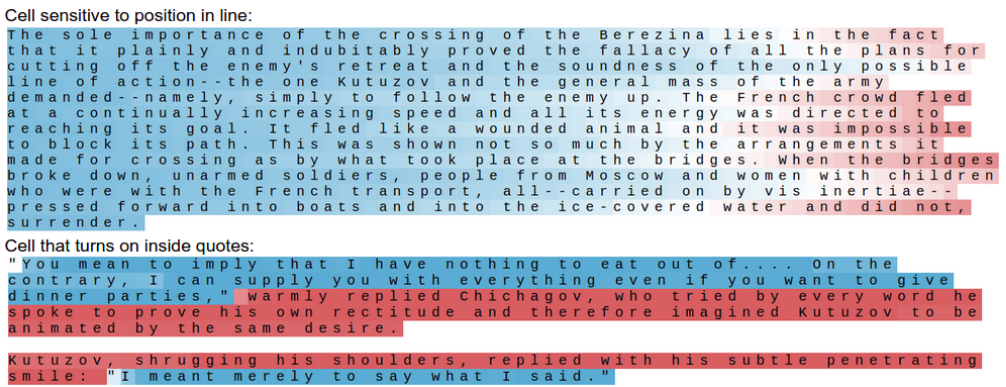
\includegraphics[width=\textwidth]{images/karpathy}
%
%\url{http://karpathy.github.io/2015/05/21/rnn-effectiveness/}
%\end{frame}


\input{images/activations.tikz}
\begin{frame}
\frametitle{Internal States Encode increasingly Classification Features}
\framesubtitle{LSTM cell \textbf{47} of 256}
\figactivations{1}{3}
\end{frame}
%%
%
\begin{frame}
\frametitle{Found Cloud Masking Cells in the RNN}
\framesubtitle{LSTM cell \textbf{47} of 256}
\figactivations{1}{47}
\end{frame}

\begin{frame}
\frametitle{Gate Activations are complicated}

\begin{itemize}
\item something seems to happen with the gates given the input
\item hard to visually interpret
\item still classification accuracy circa 80\% $\leftarrow$ gates seem to follow a purpose
\item information likely encoded in a linear combination in multiple dimensions over multiple layers
\item the designed purpose of the gates \emph{input},\emph{forget},\emph{output}, etc. may not be very meaningful
\end{itemize}
\end{frame}

{\setbeamercolor{background canvas}{bg=tumbluedark}
\begin{frame}[plain]

\vspace{8em}
\begin{center}
\Huge\color{tumwhite}
One more tool in our Deep Learning toolbox....
\end{center}\color{white}

\end{frame}
}

{\setbeamercolor{background canvas}{bg=white}
\begin{frame}[plain]

\vspace{8em}
\begin{center}
\Huge\color{tumbluedark}
Gradients
\end{center}\color{white}

\end{frame}
}

\begin{frame}
\only<1-3>{\frametitle{Usually we use gradients to adjust $\Mweight$...}}
\only<4->{\frametitle{We can also backprop to $\M{X}$}}

\begin{tikzpicture}
\node[font=\Huge](grad){
\only<1-3>{
$\frac{\partial \mathcal{L}(\V{y},f_\Mweight(\M{X}))}{\partial \Mweight}$
}
\only<4->{
$\frac{\partial \max(\yhat)}{\partial \M{X}}$
}
};

\node[above left=of grad, text width=12em](annotdx){
\only<2,3>{how do we have to change the network weights $\Mweight$...}
\only<4,5>{what changes in the input $\M{X}$...} 
};
\node[below right=of grad, text width=12em](annotdy){
\only<3>{... to change (minimize) the loss $\mathcal{L}$?}
\only<5>{... would change the predicted score $\max(\yhat) = \max(\f_\Mweight(\VInput))$?}
};

\visible<2,3,4,5>{\draw[-stealth, shorten >= 1em, rounded corners] (annotdx) -| ($ (annotdx)!0.5!(grad) $) |- ($ (grad)+(-.5em, -1em) $);}
\visible<3,5>{\draw[-stealth, shorten >= 1em, rounded corners] (annotdy) -| ($ (annotdy)!0.5!(grad) $) |- ($ (grad)+(2.5em, 1em) $);}

\end{tikzpicture}
\end{frame}


\begin{frame}
\begin{tikzpicture}

\frametitle{Gradients from $\max(\yhat)$ to \M{X}}
\framesubtitle{Example 1}


\def\root{images/rnn_examples/5}


\begin{groupplot}[
group style = {
group size = 1 by 3,
xlabels at=edge bottom,
xticklabels at=edge bottom,
vertical sep=0pt,
},
width=\textwidth,
%		hide axis,
enlargelimits=.1,
height=4cm,
%ymin=-.2, ymax=.2,
%no marks,
]
\nextgroupplot[draw opacity=.8, smooth=0.01, ylabel=$\M{X}$]
\addplot[b11color, mark=*,mark size=.5pt] table [x=t, y=B11, col sep=comma, forget plot] {\root/x.csv};
\addplot[b12color, mark=*,mark size=.5pt] table [x=t, y=B12, col sep=comma] {\root/x.csv};

\addplot[b5color, mark=*,mark size=.5pt] table [x=t, y=B5, col sep=comma, forget plot] {\root/x.csv};
\addplot[b6color, mark=*,mark size=.5pt] table [x=t, y=B6, col sep=comma, forget plot] {\root/x.csv};
\addplot[b7color, mark=*,mark size=.5pt] table [x=t, y=B7, col sep=comma, forget plot] {\root/x.csv};
\addplot[b8color, mark=*,mark size=.5pt] table [x=t, y=B8, col sep=comma, forget plot] {\root/x.csv};
\addplot[b8Acolor, mark=*,mark size=.5pt] table [x=t, y=B8A, col sep=comma] {\root/x.csv};

\addplot[b2color, mark=*,mark size=.5pt] table [x=t, y=B2, col sep=comma, forget plot] {\root/x.csv};
\addplot[b3color, mark=*,mark size=.5pt] table [x=t, y=B3, col sep=comma, forget plot] {\root/x.csv};
\addplot[b4color, mark=*,mark size=.5pt] table [x=t, y=B4, col sep=comma] {\root/x.csv};

\nextgroupplot[draw opacity=.8, smooth=0.01, ylabel=$\frac{\partial \max(\yhat)}{\partial \V{X}}$]
\addplot[b11color, mark=*,mark size=.5pt] table [x=t, y=B11, col sep=comma, forget plot] {\root/dydx.csv};
\addplot[b12color, mark=*,mark size=.5pt] table [x=t, y=B12, col sep=comma] {\root/dydx.csv};

\addplot[b5color, mark=*,mark size=.5pt] table [x=t, y=B5, col sep=comma, forget plot] {\root/dydx.csv};
\addplot[b6color, mark=*,mark size=.5pt] table [x=t, y=B6, col sep=comma, forget plot] {\root/dydx.csv};
\addplot[b7color, mark=*,mark size=.5pt] table [x=t, y=B7, col sep=comma, forget plot] {\root/dydx.csv};
\addplot[b8color, mark=*,mark size=.5pt] table [x=t, y=B8, col sep=comma, forget plot] {\root/dydx.csv};
\addplot[b8Acolor, mark=*,mark size=.5pt] table [x=t, y=B8A, col sep=comma] {\root/dydx.csv};

\addplot[b2color, mark=*,mark size=.5pt] table [x=t, y=B2, col sep=comma, forget plot] {\root/dydx.csv};
\addplot[b3color, mark=*,mark size=.5pt] table [x=t, y=B3, col sep=comma, forget plot] {\root/dydx.csv};
\addplot[b4color, mark=*,mark size=.5pt] table [x=t, y=B4, col sep=comma] {\root/dydx.csv};

\end{groupplot}
\end{tikzpicture}
\end{frame}


\begin{frame}
\begin{tikzpicture}

\frametitle{Gradients from $\max(\yhat)$ to \M{X}}
\framesubtitle{Example 2}

\def\root{images/rnn_examples/6}


\begin{groupplot}[
group style = {
group size = 1 by 3,
xlabels at=edge bottom,
xticklabels at=edge bottom,
vertical sep=0pt,
},
width=\textwidth,
%		hide axis,
enlargelimits=.1,
height=4cm,
%ymin=-.2, ymax=.2,
%no marks,
]
\nextgroupplot[draw opacity=.8, smooth=0.01, ylabel=$\M{X}$]
\addplot[b11color, mark=*,mark size=.5pt] table [x=t, y=B11, col sep=comma, forget plot] {\root/x.csv};
\addplot[b12color, mark=*,mark size=.5pt] table [x=t, y=B12, col sep=comma] {\root/x.csv};

\addplot[b5color, mark=*,mark size=.5pt] table [x=t, y=B5, col sep=comma, forget plot] {\root/x.csv};
\addplot[b6color, mark=*,mark size=.5pt] table [x=t, y=B6, col sep=comma, forget plot] {\root/x.csv};
\addplot[b7color, mark=*,mark size=.5pt] table [x=t, y=B7, col sep=comma, forget plot] {\root/x.csv};
\addplot[b8color, mark=*,mark size=.5pt] table [x=t, y=B8, col sep=comma, forget plot] {\root/x.csv};
\addplot[b8Acolor, mark=*,mark size=.5pt] table [x=t, y=B8A, col sep=comma] {\root/x.csv};

\addplot[b2color, mark=*,mark size=.5pt] table [x=t, y=B2, col sep=comma, forget plot] {\root/x.csv};
\addplot[b3color, mark=*,mark size=.5pt] table [x=t, y=B3, col sep=comma, forget plot] {\root/x.csv};
\addplot[b4color, mark=*,mark size=.5pt] table [x=t, y=B4, col sep=comma] {\root/x.csv};

\nextgroupplot[draw opacity=.8, smooth=0.01, ylabel=$\frac{\partial \max(\yhat)}{\partial \V{X}}$]
\addplot[b11color, mark=*,mark size=.5pt] table [x=t, y=B11, col sep=comma, forget plot] {\root/dydx.csv};
\addplot[b12color, mark=*,mark size=.5pt] table [x=t, y=B12, col sep=comma] {\root/dydx.csv};

\addplot[b5color, mark=*,mark size=.5pt] table [x=t, y=B5, col sep=comma, forget plot] {\root/dydx.csv};
\addplot[b6color, mark=*,mark size=.5pt] table [x=t, y=B6, col sep=comma, forget plot] {\root/dydx.csv};
\addplot[b7color, mark=*,mark size=.5pt] table [x=t, y=B7, col sep=comma, forget plot] {\root/dydx.csv};
\addplot[b8color, mark=*,mark size=.5pt] table [x=t, y=B8, col sep=comma, forget plot] {\root/dydx.csv};
\addplot[b8Acolor, mark=*,mark size=.5pt] table [x=t, y=B8A, col sep=comma] {\root/dydx.csv};

\addplot[b2color, mark=*,mark size=.5pt] table [x=t, y=B2, col sep=comma, forget plot] {\root/dydx.csv};
\addplot[b3color, mark=*,mark size=.5pt] table [x=t, y=B3, col sep=comma, forget plot] {\root/dydx.csv};
\addplot[b4color, mark=*,mark size=.5pt] table [x=t, y=B4, col sep=comma] {\root/dydx.csv};

\end{groupplot}
\end{tikzpicture}
\end{frame}


\begin{frame}
\begin{tikzpicture}

\frametitle{Gradients from $\max(\yhat)$ to \M{X}}
\framesubtitle{Example 3}

\def\root{images/rnn_examples/7}


\begin{groupplot}[
group style = {
group size = 1 by 3,
xlabels at=edge bottom,
xticklabels at=edge bottom,
vertical sep=0pt,
},
width=\textwidth,
%		hide axis,
enlargelimits=.1,
height=4cm,
%ymin=-.2, ymax=.2,
%no marks,
]
\nextgroupplot[draw opacity=.8, smooth=0.01, ylabel=$\M{X}$]
\addplot[b11color, mark=*,mark size=.5pt] table [x=t, y=B11, col sep=comma, forget plot] {\root/x.csv};
\addplot[b12color, mark=*,mark size=.5pt] table [x=t, y=B12, col sep=comma] {\root/x.csv};

\addplot[b5color, mark=*,mark size=.5pt] table [x=t, y=B5, col sep=comma, forget plot] {\root/x.csv};
\addplot[b6color, mark=*,mark size=.5pt] table [x=t, y=B6, col sep=comma, forget plot] {\root/x.csv};
\addplot[b7color, mark=*,mark size=.5pt] table [x=t, y=B7, col sep=comma, forget plot] {\root/x.csv};
\addplot[b8color, mark=*,mark size=.5pt] table [x=t, y=B8, col sep=comma, forget plot] {\root/x.csv};
\addplot[b8Acolor, mark=*,mark size=.5pt] table [x=t, y=B8A, col sep=comma] {\root/x.csv};

\addplot[b2color, mark=*,mark size=.5pt] table [x=t, y=B2, col sep=comma, forget plot] {\root/x.csv};
\addplot[b3color, mark=*,mark size=.5pt] table [x=t, y=B3, col sep=comma, forget plot] {\root/x.csv};
\addplot[b4color, mark=*,mark size=.5pt] table [x=t, y=B4, col sep=comma] {\root/x.csv};

\nextgroupplot[draw opacity=.8, smooth=0.01, ylabel=$\frac{\partial \max(\yhat)}{\partial \V{X}}$]
\addplot[b11color, mark=*,mark size=.5pt] table [x=t, y=B11, col sep=comma, forget plot] {\root/dydx.csv};
\addplot[b12color, mark=*,mark size=.5pt] table [x=t, y=B12, col sep=comma] {\root/dydx.csv};

\addplot[b5color, mark=*,mark size=.5pt] table [x=t, y=B5, col sep=comma, forget plot] {\root/dydx.csv};
\addplot[b6color, mark=*,mark size=.5pt] table [x=t, y=B6, col sep=comma, forget plot] {\root/dydx.csv};
\addplot[b7color, mark=*,mark size=.5pt] table [x=t, y=B7, col sep=comma, forget plot] {\root/dydx.csv};
\addplot[b8color, mark=*,mark size=.5pt] table [x=t, y=B8, col sep=comma, forget plot] {\root/dydx.csv};
\addplot[b8Acolor, mark=*,mark size=.5pt] table [x=t, y=B8A, col sep=comma] {\root/dydx.csv};

\addplot[b2color, mark=*,mark size=.5pt] table [x=t, y=B2, col sep=comma, forget plot] {\root/dydx.csv};
\addplot[b3color, mark=*,mark size=.5pt] table [x=t, y=B3, col sep=comma, forget plot] {\root/dydx.csv};
\addplot[b4color, mark=*,mark size=.5pt] table [x=t, y=B4, col sep=comma] {\root/dydx.csv};

\end{groupplot}
\end{tikzpicture}
\end{frame}

\begin{frame}
	\frametitle{Jupyter Notebook}
	
	
	\Large
	\textbf{github.com/marccoru/phiweek19/recurrence.ipynb}
	
	\vspace{1em}
	
	\Large $\frac{\partial \max(\yhat)}{\partial \M{X}}$ implementation
	
	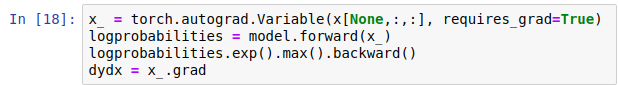
\includegraphics[width=\textwidth]{images/dydx_code}
	
\end{frame}
%
%\def\fps{3}
%\input{images/cells.tikz}
%
%\begin{frame}[t]
%\frametitle{Extracting features from noisy data with ConvRNNs}
%
%\centering
%%\lstmanim
%\begin{tikzpicture}[scale=1, node distance=2em]%,show background rectangle,background rectangle/.style={draw=red}]
%
%
%\draw pic (LSTM) at (0,0) {lstmanim};
%\node[io,xshift=1ex,above=3em of LSTMtl, ,label=above:$\VInput_{t}$](xt){\animategraphics[poster=25,width=1cm,autoplay,loop]{\fps}{images/activations/16494/x/x-}{1}{36}};%$x_{t}$
%\draw[rounded corners] (xt) |- (LSTM-input);
%\node[io,left=of LSTMtl,label=below:$\VHidden_{t-1}$](htminus1){
%	\animategraphics[poster=24,width=1cm,autoplay,loop]{\fps}{images/activations/16494/output/3-}{0}{35}
%};
%\draw[endflow] (htminus1) -- (LSTM-input);
%\node[io,right=of LSTMbr,label=above:$\VCellState_{t}$](ct){\animategraphics[poster=25,width=1cm,autoplay,loop]{\fps}{images/activations/16494/state/3-}{1}{36}}; % $c_{t}$
%\draw[endflow] (LSTM-coutput)--(ct);
%\node[io,left=of LSTMbl,label=above:$\VCellState_{t-1}$](ctminus1){\animategraphics[poster=24,width=1cm,autoplay,loop]{\fps}{images/activations/16494/state/3-}{0}{35}}; % 
%\draw[endflow] (ctminus1)--(LSTMfmult);
%\node[io,right=of LSTMtr,label=below:$\VHidden_{t}$](ht){
%	\animategraphics[poster=24,width=1cm,autoplay,loop]{\fps}{images/activations/16494/output/3-}{1}{36}
%%};
%\draw[endflow] (LSTM-houtput)--(ht);
%
%\draw[endflow] (ct) -- ($ (ct)+(0,-0.8) $) -| (ctminus1);
%\draw[endflow] (ht) -- ($ (ht)+(0,.8) $) -| (htminus1);
%
%\end{tikzpicture}
%
%\end{frame}


{\setbeamercolor{background canvas}{bg=black}
	\begin{frame}[plain]
	\vfill
	\begin{columns}
		\column{.5\textwidth}
		\color{tumwhite}
		
		\Huge
		\visible<2->{\color{tumgray} Self-}{\color{white}Attention} \visible<2->{in \\ Deep Learning}
		
		\column{.5\textwidth}
		
		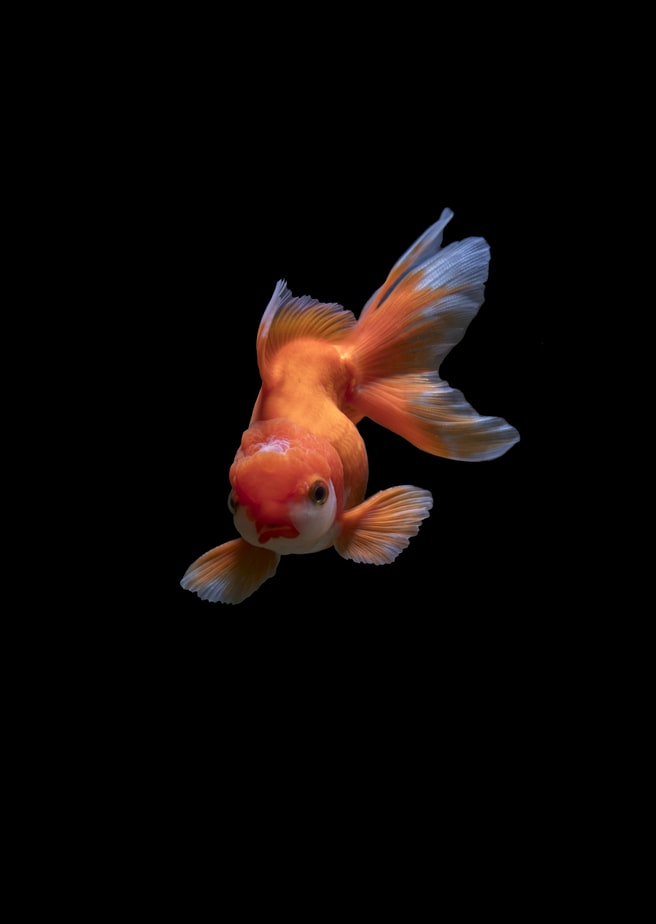
\includegraphics[width=6cm]{images/goldfish_zhengtaoTang}
	\end{columns}
	\begin{center}
		\Huge\color{tumwhite}
		\vfill\raggedleft
		{\small \color{tumgray} Photo by zhengtao tang on Unsplash}
		
	\end{center}
	\vfill
\end{frame}
}

\begin{frame}
	\frametitle{Attention}
	
	\begin{columns}
		\column{.5\textwidth}
		
%		
%		
%		\attention
%		
%		\attnv
		
		\begin{tikzpicture}[node distance=.2em]
		\node[label={below:$\V{\alpha}^T$}, draw=attentioncolor, rounded corners](alpha){\attention};
		\node[right=of alpha](out){\attnout};
		\node[above=of out, label={above:${\only<1,2>{\V{v}}\only<3>{\M{V}}}$}, draw=valuecolor, rounded corners]{\attnv};
		\visible<2->{
		\node[above=of alpha, label={above:$\M{K}$}, draw=keycolor, rounded corners]{\attnkey};
		\node[left=of alpha, label={below:${\only<1,2>{\V{q}}\only<3>{\M{Q}}}^T$}, draw=querycolor, rounded corners]{\attnquery};
		}
		\end{tikzpicture}
		
		%	\begin{equation*}
		%		\text{Attention}(Q,K,V) = 
		%		\begin{tikzpicture}
		%		\node(alpha){$\underbrace{\attention}_\alpha$};
		%		\node[right=of alpha](out){};
		%		\node[above=of out]{\attnv};
		%		\end{tikzpicture}
		%		 
		%	\end{equation*}
		
		
		\column{.5\textwidth}
		
		\begin{tikzpicture}[yscale=3]
			
			\visible<3>{
				\node[draw=valuecolor, circle, fill=valuecolor, fill opacity=.2, text opacity=1, font=\small, inner sep=.2em](d) at (1,.35){};
				\node[draw=valuecolor, circle, fill=valuecolor, fill opacity=.1, text opacity=1, font=\small, inner sep=.2em](e) at (2,.05){};
				\node[draw=valuecolor, circle, fill=valuecolor, fill opacity=.3, text opacity=1, font=\small, inner sep=.2em](f) at (3,.42){};
				\node[draw=valuecolor, circle, fill=valuecolor, fill opacity=.4, text opacity=1, font=\small, inner sep=.2em](g) at (4,.25){};
				\draw (d) -- (e) -- (f) -- (g);
			}
			
			\node[draw=valuecolor, circle, fill=valuecolor, fill opacity=.2, text opacity=1, font=\small, inner sep=.2em](a) at (1,.3){};
			\node[draw=valuecolor, circle, fill=valuecolor, fill opacity=.1, text opacity=1, font=\small, inner sep=.2em](b) at (2,.1){};
			\node[draw=valuecolor, circle, fill=valuecolor, fill opacity=.3, text opacity=1, font=\small, inner sep=.2em](c) at (3,.3){};
			\node[draw=valuecolor, circle, fill=valuecolor, fill opacity=.4, text opacity=1, font=\small, inner sep=.2em](d) at (4,.4){};
			
			\draw (a) -- (b) -- (c) -- (d);
			
			\foreach \t in {1,2,3,4} {
				\draw[tumgray] (\t,0) -- (\t,-.05) node[at end, below, text=tumgray] {$t_\t$};
			}
			
			%\draw[-stealth] (0,0) -- (0,.5);
			\draw[-stealth, tumgray] (.5,0) -- (4.5,0);
			
			\only<1,2>{
			\node[draw=tumblack, circle, fill=attentionoutcolor, text=white, fill opacity=1, text opacity=1, font=\small, inner sep=.2em, label={right:$\sum_{t=0}^{T} \alpha_t v_t = \V{\alpha}^T \V{v}$}](out) at (2.5,-.5) {};
			}
			\only<3>{
			\node[draw=white, circle, fill=attentionoutcolor, text=white, fill opacity=1, text opacity=1, font=\small, inner sep=.2em](outba) at (1.05,-.48) {};
			\node[draw=white, circle, fill=attentionoutcolor, text=white, fill opacity=1, text opacity=1, font=\small, inner sep=.2em](outbb) at (2.05,-.48) {};
			\node[draw=white, circle, fill=attentionoutcolor, text=white, fill opacity=1, text opacity=1, font=\small, inner sep=.2em](outbc) at (3.05,-.48) {};
			\node[draw=white, circle, fill=attentionoutcolor, text=white, fill opacity=1, text opacity=1, font=\small, inner sep=.2em](outbd) at (4.05,-.48) {};
				
			\node[draw=white, circle, fill=attentionoutcolor, text=white, fill opacity=1, text opacity=1, font=\small, inner sep=.2em](outa) at (1,-.5) {};
			\node[draw=white, circle, fill=attentionoutcolor, text=white, fill opacity=1, text opacity=1, font=\small, inner sep=.2em](out) at (2,-.5) {};
			\node[draw=white, circle, fill=attentionoutcolor, text=white, fill opacity=1, text opacity=1, font=\small, inner sep=.2em](outa) at (3,-.5) {};
			\node[draw=white, circle, fill=attentionoutcolor, text=white, fill opacity=1, text opacity=1, font=\small, inner sep=.2em](outa) at (4,-.5) {};

			}
		
			\node at (2.5, -.25) {};
			
			\draw[-stealth, draw=tumred, opacity=.4, line width=.4] (a) -- (out);
			\draw[-stealth, draw=tumred, opacity=.8, line width=.8] (b) -- (out);
			\draw[-stealth, draw=tumred, opacity=.2, line width=.2] (c) -- (out);
			\draw[-stealth, draw=tumred, opacity=.6, line width=.6] (d) -- (out);
			
			\node(annot1) at (5.5,.1){keep those};
			\draw[-stealth, tumred, shorten <= .3em, , shorten >= .3em](annot1) -- (b);
			\draw[-stealth, tumred, shorten <= .3em, , shorten >= .3em](annot1) -- (d);
			
			\node(annot2) at (3.5,.85){ignore these};
			\draw[-stealth, tumbluelight, shorten <= 1em, shorten >= 1em](annot2) -- (a);
			\draw[-stealth, tumbluelight, shorten <= 1em, shorten >= 1em](annot2) -- (c);
			
			
		\end{tikzpicture}
%		
%		
%		\begin{tikzpicture}
%		\begin{axis}[height=3cm,width=\textwidth,grid=major,]
%		\addplot coordinates {(0,.3) (1,.1) (2,.3) (3,.4)};
%		\end{axis}
%		\end{tikzpicture}
%		\begin{tikzpicture}
%			
%			\begin{axis}[ybar,height=3cm,width=\textwidth,grid=major,]
%			\addplot coordinates {(1,.05) (0,.4) (3,.05) (2,.5)};
%			\end{axis}
%		\end{tikzpicture}
	\end{columns}

	
	\Large
	\only<1>{
	\begin{equation*}
	\text{Attention}({\color{tumred}\V{\alpha}}, {\color{tumblue}\V{v}}) = {\color{tumred}\V{\alpha}}^T  {\color{tumblue}\V{v}} = \sum_{t=0}^{T} \alpha_tv_t, \quad \V{\alpha} \in [0,1]^{T=4}, \V{v} \in \mathbb{R}^{T}
	\end{equation*}
	}
	\only<2>{
		\begin{equation*}
		\text{Attention}({\color{tumorange}\V{K}}, {\color{tumgreen}\V{q}}, {\color{tumblue}\V{v}}) = 
		\overbrace{\text{softmax}\left({\color{tumgreen}\V{q}^T}{\color{tumorange}\V{K}}\right)}^{{\color{tumred}\V{\alpha}}^T}
		{\color{tumblue}\V{v}}, \quad \V{v} \in \mathbb{R}^{T}, \V{q} \in \mathbb{R}^{D_k}, \M{K} \in \mathbb{R}^{D_k \times T}
		\end{equation*}
	}
	\only<3>{
		\begin{equation*}
		\text{Attention}({\color{tumorange}\V{K}}, {\color{tumgreen}\V{Q}}, {\color{tumblue}\V{V}}) = 
		\text{softmax}\left({\color{tumgreen}\V{Q}^T}{\color{tumorange}\V{K}}\right)
		{\color{tumblue}\V{V}}, \quad \V{V} \in \mathbb{R}^{T \times D_v}, \V{Q} \in \mathbb{R}^{D_k \times T}, \M{K} \in \mathbb{R}^{D_k \times T}
		\end{equation*}
	}
\end{frame}


\begin{frame}
	
	
	\begin{equation*}
	\text{Attention}(Q,K,V) = \underbrace{\text{softmax}\left(QK^T\right)}_\alpha V
	\end{equation*}
	query: $Q \in \mathbb{R}^{t \times d_k}$
	
	key: $K \in \mathbb{R}^{t \times d_k}$
	
	value: $V \in \mathbb{R}^{t \times d_v}$
	
	attention scores $\alpha \in [0,1]^{t \times t}$
	
	
\end{frame}


\begin{frame}
	\frametitle{test}
	
	\tikzstyle{conn} = [-stealth, rounded corners, tumbluedark, thick]
	\tikzstyle{module} = [draw=none, fill=tumgraylight, rounded corners]
	\tikzstyle{layer} = [draw=none, fill=tumbluelight, rounded corners]
	
	\visible<2>{
	\begin{tikzpicture}[node distance=2em]
		\node(input){inputs};
		\node[below of=input](plus){+};
		\node[left of=plus](posenc){p};
		
		\node[module, below=2em of plus](attn){Multi-Head-Attention};
		\node[module, below=.5em of attn](addnorm){Add \& Norm};
		
		\node[module, below=2em of addnorm](ff){Feed Forward};
		\node[module, below=.5em of ff](addnorm2){Add \& Norm};
		
		
		\coordinate[above=of attn](in);
		\coordinate[below=of addnorm2](out);
		\draw[conn] (in) -- (attn);
		\draw[conn] (in) -- ($ (attn)!.5!(in) $) -| ($ (attn.north)+(2em,0) $);
		\draw[conn] (in) -- ($ (attn)!.5!(in) $) -| ($ (attn.north)-(2em,0) $);  
%		
		\draw[conn] (in) -- ($ (attn)!.6!(in) $) -| ($ (attn.east)+(.5em,0) $) |- (addnorm.east);

		\draw[conn] (attn) -- (addnorm);
		
		\draw[conn] (addnorm) -- (ff);
		\draw[conn] (addnorm) -- ($ (addnorm)!.5!(ff) $) -| ($ (ff.east)+(.5em,0) $) |- (addnorm2.east);
		\draw[conn] (ff) -- (addnorm2);
		\draw[conn] (addnorm2) -- (out);
		
		\begin{pgfonlayer}{background}
			\node[layer, draw=black, fit=(attn)(addnorm)(ff)(addnorm2)(in)(out)]{};
		\end{pgfonlayer}
		
	\end{tikzpicture}
}
	
\end{frame}


{\setbeamercolor{background canvas}{bg=tumbluedark}
	\begin{frame}[plain]
	\vfill
	\begin{center}
		\Huge\color{tumwhite}
		Quantitative Experimental Results
	\end{center}
	\vfill
\end{frame}
}


\begin{frame}
	\frametitle{Dataset}

	
	\begin{tikzpicture}[node distance=.5em]
	\node(raw1){\rawtimeseriestwo{12-71456800_raw.csv}};
	\node[right=of raw1](pre1){\rawtimeseriestwo{12-71456800.csv}};
	
	\node[below=of raw1](raw2){\rawtimeseriestwo{27-71460091_raw.csv}};
	\node[right=of raw2](pre2){\rawtimeseriestwo{27-71460091.csv}};
	
	\node[above=of raw1]{Raw Sentinel 2 Data};
	\node[above=of pre1]{\includegraphics[width=1cm]{images/GAF_logo}-preprocessed Sentinel 2 Data};
	
	\node[left=of raw1]{meadow};
	\node[left=of raw2]{wheat};
	\end{tikzpicture}
	
%
%\begin{tabular}{lcc}
%	\toprule
%	Datasets & Raw Sentinel 2 Data & \includegraphics[width=1cm]{images/GAF_logo}-preprocessed Sentinel 2 Data \\
%	\cmidrule(lr){2-2}\cmidrule(lr){3-3}
%	{\vspace{1em}meadow} &  & \rawtimeseriestwo{12-71456800.csv} \\
%	{wheat} & \rawtimeseriestwo{27-71460091_raw.csv} & \rawtimeseriestwo{27-71460091.csv} \\
%	{32 more} & \rawtimeseriestwo{1-71470174_raw.csv} & \rawtimeseriestwo{1-71470174.csv} \\
%	\bottomrule
%\end{tabular}

%\begin{columns}[t]
%	
%	\column{.5\textwidth}
%	Raw Sentinel 2 Data
%	
%	\rawtimeseriestwo{12-71456800_raw.csv}
%	
%	\column{.5\textwidth}
%	\includegraphics[width=2cm]{images/GAF_logo}-preprocessed Sentinel 2 Data
%	
%	\rawtimeseriestwo{12-71456800.csv}
%	
%\end{columns}

%	\begin{tikzpicture}[baseline=-2em, inner sep=0]
%
%\begin{axis}[
%thin,
%width=6cm,
%%hide axis,
%height=3cm,
%ymin=0, ymax=1.4,
%no marks,  
%draw opacity=.8,
%smooth=0.01
%]
%%
%%
%\addplot[b11color] table [x=t, y=B11, col sep=comma, forget plot] {images/example/12-71456800_raw.csv};
%\addplot[b12color] table [x=t, y=B12, col sep=comma] {images/example/12-71456800_raw.csv};
%
%\addplot[b5color] table [x=t, y=B05, col sep=comma, forget plot] {images/example/12-71456800_raw.csv};
%\addplot[b6color] table [x=t, y=B06, col sep=comma, forget plot] {images/example/12-71456800_raw.csv};
%\addplot[b7color] table [x=t, y=B07, col sep=comma, forget plot] {images/example/12-71456800_raw.csv};
%\addplot[b8color] table [x=t, y=B08, col sep=comma, forget plot] {images/example/12-71456800_raw.csv};
%\addplot[b8Acolor] table [x=t, y=B8A, col sep=comma] {images/example/12-71456800_raw.csv};
%
%\addplot[b2color] table [x=t, y=B02, col sep=comma, forget plot] {images/example/12-71456800_raw.csv};
%\addplot[b3color] table [x=t, y=B03, col sep=comma, forget plot] {images/example/12-71456800_raw.csv};
%\addplot[b4color] table [x=t, y=B04, col sep=comma] {images/example/12-71456800_raw.csv};
%
%\end{axis}
%
%\end{tikzpicture}
\end{frame}


\begin{frame}
\frametitle{Models}

\centering\begin{tabular}{lcccc}
	\toprule
	& LSTM-RNN$^1$ & Transformer$^1$ & MS-ResNet$^3$ & TempCNN$^4$ \\
	\cmidrule(lr){2-2}\cmidrule(lr){3-3}\cmidrule(lr){4-4}\cmidrule(lr){5-5}
	Mechanism & Recurrence & Self-Attention & Convolution & Convolution \\
	Parameter & 100k & 600k & 2Mio & 433k \\
	\bottomrule
\end{tabular}

\vspace{2em}

{\small\raggedright

$^1$ Hochreiter, S., \& Schmidhuber, J. (1997). Long short-term memory. Neural computation, 9(8), 1735-1780.

$^2$ Vaswani, A., Shazeer, N., Parmar, N., Uszkoreit, J., Jones, L., Gomez, A. N., ... \& Polosukhin, I. (2017). Attention is all you need. In Advances in neural information processing systems (pp. 5998-6008).

$^3$ Wang, F., Han, J., Zhang, S., He, X., \& Huang, D. (2018). Csi-net: Unified human body characterization and action recognition. arXiv preprint arXiv:1810.03064.

$^4$ Pelletier, C., Webb, G. I., \& Petitjean, F. (2019). Temporal convolutional neural network for the classification of satellite image time series. Remote Sensing, 11(5), 523.

}

\end{frame}


\begin{frame}
\frametitle{Preprocessed versus Raw Data (Sentinel 2, Region Holl)}

\begin{tabular}{rrlrlrlrl}
	\toprule
	& \multicolumn{2}{c}{MS-ResNet} & \multicolumn{2}{c}{RNN (LSTM)} & \multicolumn{2}{c}{Transformer} & \multicolumn{2}{c}{TempCNN} \\
	& acc. & $\kappa$ & acc. & $\kappa$ & acc. & $\kappa$ & acc. & $\kappa$ \\
	\cmidrule(lr){2-3}\cmidrule(lr){4-5} \cmidrule(lr){6-7}\cmidrule(lr){8-9}
	preprocessed & \textbf{0.8654} & \textbf{0.8360} & 0.7997 & 0.7513 & \textbf{0.8647} & \textbf{0.8363} & \textbf{0.8407} & \textbf{0.8034} \\
	raw 		 & 0.8331 & 0.7971 & \textbf{0.8048} & \textbf{0.7611} & 0.7859 & 0.7420 & 0.7944 & 0.7462 \\
	\bottomrule
\end{tabular}

\end{frame}



%

{\setbeamercolor{background canvas}{bg=white}
	\begin{frame}[plain]
	
	\vspace{8em}
	\begin{center}
		\Huge\color{tumbluedark}
		\phantom{How }Should we deal with $\includegraphics[width=2em]{images/icons/cloud2_tumbluedark}^\ast$ at all?
	\end{center}\color{tumbluedark}
	\vspace{2em}
	\raggedleft \Large$^\ast$ ...and other noise in the data
	
	\vfill
	\vspace{6em}
	\raggedleft{\small \color{tumgray}
		Icons made by Smashicons from www.flaticon.com
	}
\end{frame}
}


\begin{frame}
\frametitle{Looking at single pixels}
\framesubtitle{Sentinel 2 (raw)}


\begin{tikzpicture}[baseline=-2em, inner sep=0]

\begin{axis}[
width=\textwidth,
%	hide axis,
height=5.5cm,
ymin=0, ymax=1.2,
%no marks,  
draw opacity=.8,
smooth=0.001,
legend style={at={(.65,1.1)},line width=2pt, draw opacity=1},
legend columns=3,
ylabel={reflectance},
xlabel={time $t$}
]


%\only<3->{
%	\node[draw=tumbluedark, rounded corners, inner sep=0, minimum width=.8em, minimum height=3em](xt) at (axis cs:16,0.155){};
%	\node (annotxt) at (axis cs:20,1){$\V{x}_t = 
%		\begin{pmatrix} \rho_\text{B02} \\ \dots \\ \rho_\text{B12} \end{pmatrix} = 
%		\left(\xtvector\right)$};
%	\draw[-stealth] (annotxt) -- (xt);
%}

\only<1>{
\addplot[b2color, tsmark] table [x=t, y=B02, col sep=comma]  {images/example/12-71459194_raw.csv};
\addplot[b3color, tsmark] table [x=t, y=B03, col sep=comma]  {images/example/12-71459194_raw.csv};
\addplot[b4color, tsmark] table [x=t, y=B04, col sep=comma]  {images/example/12-71459194_raw.csv};
\addplot[b5color, tsmark] table [x=t, y=B05, col sep=comma]  {images/example/12-71459194_raw.csv};
\addplot[b6color, tsmark] table [x=t, y=B06, col sep=comma]  {images/example/12-71459194_raw.csv};
\addplot[b7color, tsmark] table [x=t, y=B07, col sep=comma]  {images/example/12-71459194_raw.csv};
\addplot[b8color, tsmark] table [x=t, y=B08, col sep=comma]  {images/example/12-71459194_raw.csv};
\addplot[b8Acolor, tsmark] table [x=t, y=B8A, col sep=comma] {images/example/12-71459194_raw.csv};
\addplot[b11color, tsmark] table [x=t, y=B11, col sep=comma] {images/example/12-71459194_raw.csv};
\addplot[b12color, tsmark] table [x=t, y=B12, col sep=comma] {images/example/12-71459194_raw.csv};
\node[font=\Large](classannot) at (axis cs:25,1.1) {\textbf{meadow} \small(parcel 71459194)};
}

\only<2->{
\addplot[b2color, tsmark] table [x=t, y=B02, col sep=comma]  {images/example/27-71460294_raw.csv};
\addplot[b3color, tsmark] table [x=t, y=B03, col sep=comma]  {images/example/27-71460294_raw.csv};
\addplot[b4color, tsmark] table [x=t, y=B04, col sep=comma]  {images/example/27-71460294_raw.csv};
\addplot[b5color, tsmark] table [x=t, y=B05, col sep=comma]  {images/example/27-71460294_raw.csv};
\addplot[b6color, tsmark] table [x=t, y=B06, col sep=comma]  {images/example/27-71460294_raw.csv};
\addplot[b7color, tsmark] table [x=t, y=B07, col sep=comma]  {images/example/27-71460294_raw.csv};
\addplot[b8color, tsmark] table [x=t, y=B08, col sep=comma]  {images/example/27-71460294_raw.csv};
\addplot[b8Acolor, tsmark] table [x=t, y=B8A, col sep=comma] {images/example/27-71460294_raw.csv};
\addplot[b11color, tsmark] table [x=t, y=B11, col sep=comma] {images/example/27-71460294_raw.csv};
\addplot[b12color, tsmark] table [x=t, y=B12, col sep=comma] {images/example/27-71460294_raw.csv};
}
\only<2>{
\node[font=\Large](classannot) at (axis cs:25,1.1) {\textbf{wheat} \small(parcel 71460294)};
}


\end{axis}

\end{tikzpicture}

\end{frame}



\begin{frame}
\frametitle{Preprocessed versus Raw Data (Sentinel 2, Region Holl)}

\begin{tabular}{lrlrlrlrl}
\toprule
& \multicolumn{2}{c}{MS-ResNet} & \multicolumn{2}{c}{RNN (LSTM)} & \multicolumn{2}{c}{Transformer} & \multicolumn{2}{c}{TempCNN} \\
& acc. & $\kappa$ & acc. & $\kappa$ & acc. & $\kappa$ & acc. & $\kappa$ \\
\cmidrule(lr){2-3}\cmidrule(lr){4-5} \cmidrule(lr){6-7}\cmidrule(lr){8-9}
preprocessed & \textbf{0.8654} & \textbf{0.8360} & 0.7997 & 0.7513 & \textbf{0.8647} & \textbf{0.8363} & \textbf{0.8407} & \textbf{0.8034} \\
raw 		 & 0.8331 & 0.7971 & \textbf{0.8048} & \textbf{0.7611} & 0.7859 & 0.7420 & 0.7944 & 0.7462 \\
\bottomrule
\end{tabular}

\end{frame}

\begin{frame}
\frametitle{Radar}

\begin{tabular}{lrlrlrlrl}
\toprule
preprocessed data& \multicolumn{2}{c}{MS-ResNet} & \multicolumn{2}{c}{RNN (LSTM)} & \multicolumn{2}{c}{Transformer} & \multicolumn{2}{c}{TempCNN} \\
& acc. & $\kappa$ & acc. & $\kappa$ & acc. & $\kappa$ & acc. & $\kappa$ \\
\cmidrule(lr){2-3}\cmidrule(lr){4-5} \cmidrule(lr){6-7}\cmidrule(lr){8-9}
Sentinel 1 + Sentinel 2 	& x & x & 0.7983 & 0.7503 & 0.8384 & 0.8037 & x & x \\
Sentinel 2 (optical)	 	& x & x & 0.7845 & 0.7338 & 0.7936 & 0.7439 & x & x \\
Sentinel 1 (radar)		 	& x & x & 0.7305 & 0.6608 & 0.7471 & 0.6861 & x & x \\
\midrule \\
raw data \\
Sentinel 2 (optical) & 0.8331 & 0.7971 & \textbf{0.8048} & \textbf{0.7611} & 0.7859 & 0.7420 & 0.7944 & 0.7462 \\
\end{tabular}

\begin{tabular}{lrlrlrlrl}
\toprule
& \multicolumn{2}{c}{MS-ResNet} & \multicolumn{2}{c}{RNN (LSTM)} & \multicolumn{2}{c}{Transformer} & \multicolumn{2}{c}{TempCNN} \\
& acc. & $\kappa$ & acc. & $\kappa$ & acc. & $\kappa$ & acc. & $\kappa$ \\
\cmidrule(lr){2-3}\cmidrule(lr){4-5} \cmidrule(lr){6-7}\cmidrule(lr){8-9}
raw (optical)		 & 0.8331 & 0.7971 & \textbf{0.8048} & \textbf{0.7611} & 0.7859 & 0.7420 & 0.7944 & 0.7462 \\
\bottomrule
\end{tabular}

TODO experiments:
\begin{itemize}
\item multiple runs and report standard deviation
\item merge rows to one table
\end{itemize}

\end{frame}


%
\begin{frame}<presentation:4-5>
\frametitle{Let's look at a few Examples}
\framesubtitle{Sentinel 2 preprocessed by \includegraphics[width=4em]{images/GAF_logo}}


\begin{tikzpicture}[baseline=-2em, inner sep=0]

\begin{axis}[
width=\textwidth,
%	hide axis,
height=5.5cm,
ymin=0, ymax=1.2,
%no marks,  
draw opacity=.8,
smooth=0.001,
legend style={at={(.65,1.1)},line width=2pt, draw opacity=1},
legend columns=3,
ylabel={reflectance},
xlabel={time $t$}
]

\only<1,2>{
	\addplot[b2color, tsmark] table [x=t, y=B02, col sep=comma] {images/example/12-71456800.csv};
	\addplot[b3color, tsmark] table [x=t, y=B03, col sep=comma] {images/example/12-71456800.csv};
	\addplot[b4color, tsmark] table [x=t, y=B04, col sep=comma] {images/example/12-71456800.csv};
	\addplot[b5color, tsmark] table [x=t, y=B05, col sep=comma] {images/example/12-71456800.csv};
	\addplot[b6color, tsmark] table [x=t, y=B06, col sep=comma] {images/example/12-71456800.csv};
	\addplot[b7color, tsmark] table [x=t, y=B07, col sep=comma] {images/example/12-71456800.csv};
	\addplot[b8color, tsmark] table [x=t, y=B08, col sep=comma] {images/example/12-71456800.csv};
	\addplot[b8Acolor, tsmark] table [x=t, y=B8A, col sep=comma] {images/example/12-71456800.csv};
	\addplot[b11color, tsmark] table [x=t, y=B11, col sep=comma] {images/example/12-71456800.csv};
	\addplot[b12color, tsmark] table [x=t, y=B12, col sep=comma] {images/example/12-71456800.csv};
}
\only<2>{
	\node[font=\Large](classannot) at (axis cs:12,1.1) {\textbf{meadow} \small(parcel 71456800)};
}
\only<3>{
	\addplot[b2color, tsmark] table [x=t, y=B02, col sep=comma]  {images/example/12-71460758.csv};
	\addplot[b3color, tsmark] table [x=t, y=B03, col sep=comma]  {images/example/12-71460758.csv};
	\addplot[b4color, tsmark] table [x=t, y=B04, col sep=comma]  {images/example/12-71460758.csv};
	\addplot[b5color, tsmark] table [x=t, y=B05, col sep=comma]  {images/example/12-71460758.csv};
	\addplot[b6color, tsmark] table [x=t, y=B06, col sep=comma]  {images/example/12-71460758.csv};
	\addplot[b7color, tsmark] table [x=t, y=B07, col sep=comma]  {images/example/12-71460758.csv};
	\addplot[b8color, tsmark] table [x=t, y=B08, col sep=comma]  {images/example/12-71460758.csv};
	\addplot[b8Acolor, tsmark] table [x=t, y=B8A, col sep=comma] {images/example/12-71460758.csv};
	\addplot[b11color, tsmark] table [x=t, y=B11, col sep=comma] {images/example/12-71460758.csv};
	\addplot[b12color, tsmark] table [x=t, y=B12, col sep=comma] {images/example/12-71460758.csv};
	
	\node[font=\Large](classannot) at (axis cs:12,1.1) {\textbf{meadow} \small(parcel 71460758)};
}
\only<4>{
	\addplot[b2color, tsmark] table [x=t, y=B02, col sep=comma]  {images/example/12-71460855.csv};
	\addplot[b3color, tsmark] table [x=t, y=B03, col sep=comma]  {images/example/12-71460855.csv};
	\addplot[b4color, tsmark] table [x=t, y=B04, col sep=comma]  {images/example/12-71460855.csv};
	\addplot[b5color, tsmark] table [x=t, y=B05, col sep=comma]  {images/example/12-71460855.csv};
	\addplot[b6color, tsmark] table [x=t, y=B06, col sep=comma]  {images/example/12-71460855.csv};
	\addplot[b7color, tsmark] table [x=t, y=B07, col sep=comma]  {images/example/12-71460855.csv};
	\addplot[b8color, tsmark] table [x=t, y=B08, col sep=comma]  {images/example/12-71460855.csv};
	\addplot[b8Acolor, tsmark] table [x=t, y=B8A, col sep=comma] {images/example/12-71460855.csv};
	\addplot[b11color, tsmark] table [x=t, y=B11, col sep=comma] {images/example/12-71460855.csv};
	\addplot[b12color, tsmark] table [x=t, y=B12, col sep=comma] {images/example/12-71460855.csv};
	
	\node[font=\Large](classannot) at (axis cs:12,1.1) {\textbf{meadow} \small(parcel 71460855)};
}
\only<5>{
	\addplot[b2color, tsmark] table [x=t, y=B02, col sep=comma]  {images/example/27-71460091.csv};
	\addplot[b3color, tsmark] table [x=t, y=B03, col sep=comma]  {images/example/27-71460091.csv};
	\addplot[b4color, tsmark] table [x=t, y=B04, col sep=comma]  {images/example/27-71460091.csv};
	\addplot[b5color, tsmark] table [x=t, y=B05, col sep=comma]  {images/example/27-71460091.csv};
	\addplot[b6color, tsmark] table [x=t, y=B06, col sep=comma]  {images/example/27-71460091.csv};
	\addplot[b7color, tsmark] table [x=t, y=B07, col sep=comma]  {images/example/27-71460091.csv};
	\addplot[b8color, tsmark] table [x=t, y=B08, col sep=comma]  {images/example/27-71460091.csv};
	\addplot[b8Acolor, tsmark] table [x=t, y=B8A, col sep=comma] {images/example/27-71460091.csv};
	\addplot[b11color, tsmark] table [x=t, y=B11, col sep=comma] {images/example/27-71460091.csv};
	\addplot[b12color, tsmark] table [x=t, y=B12, col sep=comma] {images/example/27-71460091.csv};
	
	\node[font=\Large](classannot) at (axis cs:12,1.1) {\textbf{wheat} \small(parcel 71460091)};
}
\only<6>{
	\addplot[b2color, tsmark] table [x=t, y=B02, col sep=comma]  {images/example/27-71460294.csv};
	\addplot[b3color, tsmark] table [x=t, y=B03, col sep=comma]  {images/example/27-71460294.csv};
	\addplot[b4color, tsmark] table [x=t, y=B04, col sep=comma]  {images/example/27-71460294.csv};
	\addplot[b5color, tsmark] table [x=t, y=B05, col sep=comma]  {images/example/27-71460294.csv};
	\addplot[b6color, tsmark] table [x=t, y=B06, col sep=comma]  {images/example/27-71460294.csv};
	\addplot[b7color, tsmark] table [x=t, y=B07, col sep=comma]  {images/example/27-71460294.csv};
	\addplot[b8color, tsmark] table [x=t, y=B08, col sep=comma]  {images/example/27-71460294.csv};
	\addplot[b8Acolor, tsmark] table [x=t, y=B8A, col sep=comma] {images/example/27-71460294.csv};
	\addplot[b11color, tsmark] table [x=t, y=B11, col sep=comma] {images/example/27-71460294.csv};
	\addplot[b12color, tsmark] table [x=t, y=B12, col sep=comma] {images/example/27-71460294.csv};
	
	\node[font=\Large](classannot) at (axis cs:12,1.1) {\textbf{wheat} \small(parcel 71460294)};
}
\only<7-8>{
	\addplot[b2color, tsmark] table [x=t, y=B02, col sep=comma]  {images/example/12-71459194.csv};
	\addplot[b3color, tsmark] table [x=t, y=B03, col sep=comma]  {images/example/12-71459194.csv};
	\addplot[b4color, tsmark] table [x=t, y=B04, col sep=comma]  {images/example/12-71459194.csv};
	\addplot[b5color, tsmark] table [x=t, y=B05, col sep=comma]  {images/example/12-71459194.csv};
	\addplot[b6color, tsmark] table [x=t, y=B06, col sep=comma]  {images/example/12-71459194.csv};
	\addplot[b7color, tsmark] table [x=t, y=B07, col sep=comma]  {images/example/12-71459194.csv};
	\addplot[b8color, tsmark] table [x=t, y=B08, col sep=comma]  {images/example/12-71459194.csv};
	\addplot[b8Acolor, tsmark] table [x=t, y=B8A, col sep=comma] {images/example/12-71459194.csv};
	\addplot[b11color, tsmark] table [x=t, y=B11, col sep=comma] {images/example/12-71459194.csv};
	\addplot[b12color, tsmark] table [x=t, y=B12, col sep=comma] {images/example/12-71459194.csv};
	
}
\only<7>{
	\node[font=\Huge](classannot) at (axis cs:12,1.1) {\textbf{meadow or wheat?}};
}
\only<8>{
	\node[font=\Large](classannot) at (axis cs:12,1.1) {\textbf{meadow} \small(parcel 71459194)};
}


%
\only<1>{
	\legend{B02 (blue),B03 (green),B04 (red),B05,B06,B07,B08,B8A,B11,B12}
}

\end{axis}

\end{tikzpicture}

\end{frame}
%\begin{frame}
%\frametitle{Qualitative Examples}
%%	\framesubtitle{ConvGRU with r=256 recurrent cells}
%\centering
%\begin{tikzpicture}
%\matrix (m) [matrix of nodes, ampersand replacement=\&, row sep=0pt, column sep=2mm]{
%	$\V{x}_{RGB,t}$ \& labels $\V{y}$ \& pred. $\hat{\V{y}}$ \& $H(\V{y},\hat{\V{y}}$) \& activation \& activation \& activation \& activation
%	\tileexample{16494}{maize}{maize}{meadow}{meadow}{peas}{peas}{rape}{rape}
%	\tileexample{8133}{winter_spelt}{spelt}{winter_wheat}{wheat}{summer_barley}{s.barley}{maize}{maize}
%	\tileexample{12894}{meadow}{meadow}{winter_wheat}{wheat}{potatoe}{potato}{maize}{maize}
%	%		\tileexample{1823}{meadow}{meadow}{winter_wheat}{wheat}{summer_oat}{oat}{maize}{maize}
%	\\
%};
%\makeexamplelegend
%\end{tikzpicture}
%\end{frame}

%\begin{frame}
%\frametitle{Qualitative Examples}
%%	\framesubtitle{ConvGRU with r=256 recurrent cells}
%\centering
%\begin{tikzpicture}
%\matrix (m) [matrix of nodes, ampersand replacement=\&, row sep=0pt, column sep=2mm]{
%$\V{x}_{RGB,t}$ \& labels $\V{y}$ \& pred. $\hat{\V{y}}$ \& $H(\V{y},\hat{\V{y}}$) \& activation \& activation \& activation \& activation
%\tileexample{10879}{winter_rye}{rye}{winter_triticale}{triticale}{summer_barley}{s.barley}{winter_barley}{w.barley}
%\tileexample{10792}{winter_rye}{rye}{winter_wheat}{wheat}{winter_triticale}{triticale}{summer_barley}{s.barley}
%%		\tileexample{10969}{winter_wheat}{wheat}{winter_triticale}{triticale}{winter_rye}{rye}{rape}{rape}
%\tileexample{172}{winter_wheat}{wheat}{meadow}{meadow}{maize}{maize}{winter_barley}{w.barley}
%\\
%};
%\makeexamplelegend
%\end{tikzpicture}
%\end{frame}


%\begin{frame}
%\frametitle{How did the ConvRNN handle the cloud noise?}
%
%We performed two experiments
%\begin{enumerate}
%	\item Visualization of internal network states. We found some hidden states that were sensitive 
%\end{enumerate}
%
%\end{frame}




%\begin{frame}
%\frametitle{Looking back at the Unreasonable Effectiveness of RNNs Blog}
%\texttt{http://karpathy.github.io/2015/05/21/rnn-effectiveness/}
%\includegraphics[width=\textwidth]{images/karpathy_charrnn}
%\end{frame}

%\input{images/activations.tikz}
%\begin{frame}
%\frametitle{Cloud Sensitive Cells}
%\framesubtitle{LSTM cell \textbf{47} of 256}
%\figactivations{1}{47}
%\end{frame}
%
%\begin{frame}
%\frametitle{Ablation Experiment on Cloudy Data}
%\input{images/clouds.tikz}
%\end{frame}



\begin{frame}[c]
\frametitle{Publications and Code}
\centering 

\Large



Github + DockerHub

\vspace{1ex}

\includegraphics[width=2cm]{images/github} \hspace{.5ex}
\includegraphics[width=2cm]{images/qr_github} \hspace{.5ex}
\includegraphics[width=2cm]{images/docker}

\vspace{1ex}

\url{https://github.com/TUM-LMF/MTLCC}

\url{https://github.com/TUM-LMF/MTLCC-pytorch}

\vspace{1em}
\small
\textsl{
	Rußwurm M., Körner M. (2018). \textbf{Multi-Temporal Land Cover Classification with Sequential Recurrent Encoders}. ISPRS International Journal of Geo-Information. https://arxiv.org/abs/1802.02080.
}
	
\end{frame}


\begin{frame}
\frametitle{Cloud coverage as spatiotemporal noise}
\centering

\def\imagewidth{1.5cm}


\visible<1>{\includegraphics[width=\imagewidth]{images/activations/16494/x/x-0.png}}
\visible<1>{\includegraphics[width=\imagewidth]{images/activations/16494/x/x-1.png}}
\visible<1>{\includegraphics[width=\imagewidth]{images/activations/16494/x/x-2.png}}
\visible<1>{\includegraphics[width=\imagewidth]{images/activations/16494/x/x-3.png}}
\visible<1>{\includegraphics[width=\imagewidth]{images/activations/16494/x/x-4.png}}
\visible<1,2>{\includegraphics[width=\imagewidth]{images/activations/16494/x/x-5.png}}
\visible<1>{\includegraphics[width=\imagewidth]{images/activations/16494/x/x-6.png}}
\visible<1>{\includegraphics[width=\imagewidth]{images/activations/16494/x/x-7.png}}
\visible<1,2>{\includegraphics[width=\imagewidth]{images/activations/16494/x/x-8.png}}
\visible<1>{\includegraphics[width=\imagewidth]{images/activations/16494/x/x-9.png}}
\visible<1>{\includegraphics[width=\imagewidth]{images/activations/16494/x/x-10.png}}
\visible<1>{\includegraphics[width=\imagewidth]{images/activations/16494/x/x-11.png}}
\visible<1,2>{\includegraphics[width=\imagewidth]{images/activations/16494/x/x-12.png}}
\visible<1,2>{\includegraphics[width=\imagewidth]{images/activations/16494/x/x-13.png}}
\visible<1,2>{\includegraphics[width=\imagewidth]{images/activations/16494/x/x-14.png}}
\visible<1,2>{\includegraphics[width=\imagewidth]{images/activations/16494/x/x-15.png}}
\visible<1,2>{\includegraphics[width=\imagewidth]{images/activations/16494/x/x-16.png}}
\visible<1>{\includegraphics[width=\imagewidth]{images/activations/16494/x/x-18.png}}
\visible<1>{\includegraphics[width=\imagewidth]{images/activations/16494/x/x-19.png}}
\visible<1,2>{\includegraphics[width=\imagewidth]{images/activations/16494/x/x-20.png}}
\visible<1,2>{\includegraphics[width=\imagewidth]{images/activations/16494/x/x-21.png}}
\visible<1>{\includegraphics[width=\imagewidth]{images/activations/16494/x/x-22.png}}
\visible<1>{\includegraphics[width=\imagewidth]{images/activations/16494/x/x-23.png}}
\visible<1>{\includegraphics[width=\imagewidth]{images/activations/16494/x/x-24.png}}
\visible<1>{\includegraphics[width=\imagewidth]{images/activations/16494/x/x-25.png}}
\visible<1>{\includegraphics[width=\imagewidth]{images/activations/16494/x/x-26.png}}
\visible<1,2>{\includegraphics[width=\imagewidth]{images/activations/16494/x/x-27.png}}
\visible<1>{\includegraphics[width=\imagewidth]{images/activations/16494/x/x-28.png}}
\visible<1,2>{\includegraphics[width=\imagewidth]{images/activations/16494/x/x-29.png}}
\visible<1>{\includegraphics[width=\imagewidth]{images/activations/16494/x/x-30.png}}
\visible<1>{\includegraphics[width=\imagewidth]{images/activations/16494/x/x-31.png}}
\visible<1,2>{\includegraphics[width=\imagewidth]{images/activations/16494/x/x-32.png}}
\visible<1>{\includegraphics[width=\imagewidth]{images/activations/16494/x/x-33.png}}
%	
\end{frame}


\begin{frame}
\frametitle{Common Filtering/Preprocessing Algorithms work quite well}

\begin{columns}
	\column{.5\textwidth}
	\begin{itemize}
		\item FMask
		\item MAJA
		\item Sen2Cor (F-Mask)
		\item supervised cloud classification e.g., CNNs
		\item unsupervised cloud clustering? {\small Go FDL!}
	\end{itemize}
	\column{.5\textwidth}
	
\end{columns}
\end{frame}


\begin{frame}
\frametitle{test}

\tikzstyle{conn} = [-stealth, rounded corners, tumbluedark, thick]
\tikzstyle{module} = [draw=none, fill=tumgraylight, rounded corners]
\tikzstyle{layer} = [draw=none, fill=tumbluelight, rounded corners]

\visible<2>{
	\begin{tikzpicture}[node distance=2em]
	\node(input){inputs};
	\node[below of=input](plus){+};
	\node[left of=plus](posenc){p};
	
	\node[module, below=2em of plus](attn){Multi-Head-Attention};
	\node[module, below=.5em of attn](addnorm){Add \& Norm};
	
	\node[module, below=2em of addnorm](ff){Feed Forward};
	\node[module, below=.5em of ff](addnorm2){Add \& Norm};
	
	
	\coordinate[above=of attn](in);
	\coordinate[below=of addnorm2](out);
	\draw[conn] (in) -- (attn);
	\draw[conn] (in) -- ($ (attn)!.5!(in) $) -| ($ (attn.north)+(2em,0) $);
	\draw[conn] (in) -- ($ (attn)!.5!(in) $) -| ($ (attn.north)-(2em,0) $);  
	%		
	\draw[conn] (in) -- ($ (attn)!.6!(in) $) -| ($ (attn.east)+(.5em,0) $) |- (addnorm.east);
	
	\draw[conn] (attn) -- (addnorm);
	
	\draw[conn] (addnorm) -- (ff);
	\draw[conn] (addnorm) -- ($ (addnorm)!.5!(ff) $) -| ($ (ff.east)+(.5em,0) $) |- (addnorm2.east);
	\draw[conn] (ff) -- (addnorm2);
	\draw[conn] (addnorm2) -- (out);
	
	\begin{pgfonlayer}{background}
	\node[layer, draw=black, fit=(attn)(addnorm)(ff)(addnorm2)(in)(out)]{};
	\end{pgfonlayer}
	
	\end{tikzpicture}
}

\end{frame}


\begin{frame}
\frametitle{Let's look at a few Examples}
\framesubtitle{Sentinel 2 preprocessed by \includegraphics[width=4em]{images/GAF_logo}}


\begin{tikzpicture}[baseline=-2em, inner sep=0]

\begin{axis}[
width=\textwidth,
%	hide axis,
height=5.5cm,
ymin=0, ymax=1.2,
%no marks,  
draw opacity=.8,
smooth=0.001,
legend style={at={(.65,1.1)},line width=2pt, draw opacity=1},
legend columns=3,
ylabel={reflectance},
xlabel={time $t$}
]

\only<1,2>{
	\addplot[b2color, tsmark] table [x=t, y=B02, col sep=comma] {images/example/12-71456800.csv};
	\addplot[b3color, tsmark] table [x=t, y=B03, col sep=comma] {images/example/12-71456800.csv};
	\addplot[b4color, tsmark] table [x=t, y=B04, col sep=comma] {images/example/12-71456800.csv};
	\addplot[b5color, tsmark] table [x=t, y=B05, col sep=comma] {images/example/12-71456800.csv};
	\addplot[b6color, tsmark] table [x=t, y=B06, col sep=comma] {images/example/12-71456800.csv};
	\addplot[b7color, tsmark] table [x=t, y=B07, col sep=comma] {images/example/12-71456800.csv};
	\addplot[b8color, tsmark] table [x=t, y=B08, col sep=comma] {images/example/12-71456800.csv};
	\addplot[b8Acolor, tsmark] table [x=t, y=B8A, col sep=comma] {images/example/12-71456800.csv};
	\addplot[b11color, tsmark] table [x=t, y=B11, col sep=comma] {images/example/12-71456800.csv};
	\addplot[b12color, tsmark] table [x=t, y=B12, col sep=comma] {images/example/12-71456800.csv};
}
\only<2>{
	\node[font=\Large](classannot) at (axis cs:12,1.1) {\textbf{meadow} \small(parcel 71456800)};
}
\only<3>{
	\addplot[b2color, tsmark] table [x=t, y=B02, col sep=comma]  {images/example/12-71460758.csv};
	\addplot[b3color, tsmark] table [x=t, y=B03, col sep=comma]  {images/example/12-71460758.csv};
	\addplot[b4color, tsmark] table [x=t, y=B04, col sep=comma]  {images/example/12-71460758.csv};
	\addplot[b5color, tsmark] table [x=t, y=B05, col sep=comma]  {images/example/12-71460758.csv};
	\addplot[b6color, tsmark] table [x=t, y=B06, col sep=comma]  {images/example/12-71460758.csv};
	\addplot[b7color, tsmark] table [x=t, y=B07, col sep=comma]  {images/example/12-71460758.csv};
	\addplot[b8color, tsmark] table [x=t, y=B08, col sep=comma]  {images/example/12-71460758.csv};
	\addplot[b8Acolor, tsmark] table [x=t, y=B8A, col sep=comma] {images/example/12-71460758.csv};
	\addplot[b11color, tsmark] table [x=t, y=B11, col sep=comma] {images/example/12-71460758.csv};
	\addplot[b12color, tsmark] table [x=t, y=B12, col sep=comma] {images/example/12-71460758.csv};
	
	\node[font=\Large](classannot) at (axis cs:12,1.1) {\textbf{meadow} \small(parcel 71460758)};
}
\only<4>{
	\addplot[b2color, tsmark] table [x=t, y=B02, col sep=comma]  {images/example/12-71460855.csv};
	\addplot[b3color, tsmark] table [x=t, y=B03, col sep=comma]  {images/example/12-71460855.csv};
	\addplot[b4color, tsmark] table [x=t, y=B04, col sep=comma]  {images/example/12-71460855.csv};
	\addplot[b5color, tsmark] table [x=t, y=B05, col sep=comma]  {images/example/12-71460855.csv};
	\addplot[b6color, tsmark] table [x=t, y=B06, col sep=comma]  {images/example/12-71460855.csv};
	\addplot[b7color, tsmark] table [x=t, y=B07, col sep=comma]  {images/example/12-71460855.csv};
	\addplot[b8color, tsmark] table [x=t, y=B08, col sep=comma]  {images/example/12-71460855.csv};
	\addplot[b8Acolor, tsmark] table [x=t, y=B8A, col sep=comma] {images/example/12-71460855.csv};
	\addplot[b11color, tsmark] table [x=t, y=B11, col sep=comma] {images/example/12-71460855.csv};
	\addplot[b12color, tsmark] table [x=t, y=B12, col sep=comma] {images/example/12-71460855.csv};
	
	\node[font=\Large](classannot) at (axis cs:12,1.1) {\textbf{meadow} \small(parcel 71460855)};
}
\only<5>{
	\addplot[b2color, tsmark] table [x=t, y=B02, col sep=comma]  {images/example/27-71460091.csv};
	\addplot[b3color, tsmark] table [x=t, y=B03, col sep=comma]  {images/example/27-71460091.csv};
	\addplot[b4color, tsmark] table [x=t, y=B04, col sep=comma]  {images/example/27-71460091.csv};
	\addplot[b5color, tsmark] table [x=t, y=B05, col sep=comma]  {images/example/27-71460091.csv};
	\addplot[b6color, tsmark] table [x=t, y=B06, col sep=comma]  {images/example/27-71460091.csv};
	\addplot[b7color, tsmark] table [x=t, y=B07, col sep=comma]  {images/example/27-71460091.csv};
	\addplot[b8color, tsmark] table [x=t, y=B08, col sep=comma]  {images/example/27-71460091.csv};
	\addplot[b8Acolor, tsmark] table [x=t, y=B8A, col sep=comma] {images/example/27-71460091.csv};
	\addplot[b11color, tsmark] table [x=t, y=B11, col sep=comma] {images/example/27-71460091.csv};
	\addplot[b12color, tsmark] table [x=t, y=B12, col sep=comma] {images/example/27-71460091.csv};
	
	\node[font=\Large](classannot) at (axis cs:12,1.1) {\textbf{wheat} \small(parcel 71460091)};
}
\only<6>{
	\addplot[b2color, tsmark] table [x=t, y=B02, col sep=comma]  {images/example/27-71460294.csv};
	\addplot[b3color, tsmark] table [x=t, y=B03, col sep=comma]  {images/example/27-71460294.csv};
	\addplot[b4color, tsmark] table [x=t, y=B04, col sep=comma]  {images/example/27-71460294.csv};
	\addplot[b5color, tsmark] table [x=t, y=B05, col sep=comma]  {images/example/27-71460294.csv};
	\addplot[b6color, tsmark] table [x=t, y=B06, col sep=comma]  {images/example/27-71460294.csv};
	\addplot[b7color, tsmark] table [x=t, y=B07, col sep=comma]  {images/example/27-71460294.csv};
	\addplot[b8color, tsmark] table [x=t, y=B08, col sep=comma]  {images/example/27-71460294.csv};
	\addplot[b8Acolor, tsmark] table [x=t, y=B8A, col sep=comma] {images/example/27-71460294.csv};
	\addplot[b11color, tsmark] table [x=t, y=B11, col sep=comma] {images/example/27-71460294.csv};
	\addplot[b12color, tsmark] table [x=t, y=B12, col sep=comma] {images/example/27-71460294.csv};
	
	\node[font=\Large](classannot) at (axis cs:12,1.1) {\textbf{wheat} \small(parcel 71460294)};
}
\only<7-8>{
	\addplot[b2color, tsmark] table [x=t, y=B02, col sep=comma]  {images/example/12-71459194.csv};
	\addplot[b3color, tsmark] table [x=t, y=B03, col sep=comma]  {images/example/12-71459194.csv};
	\addplot[b4color, tsmark] table [x=t, y=B04, col sep=comma]  {images/example/12-71459194.csv};
	\addplot[b5color, tsmark] table [x=t, y=B05, col sep=comma]  {images/example/12-71459194.csv};
	\addplot[b6color, tsmark] table [x=t, y=B06, col sep=comma]  {images/example/12-71459194.csv};
	\addplot[b7color, tsmark] table [x=t, y=B07, col sep=comma]  {images/example/12-71459194.csv};
	\addplot[b8color, tsmark] table [x=t, y=B08, col sep=comma]  {images/example/12-71459194.csv};
	\addplot[b8Acolor, tsmark] table [x=t, y=B8A, col sep=comma] {images/example/12-71459194.csv};
	\addplot[b11color, tsmark] table [x=t, y=B11, col sep=comma] {images/example/12-71459194.csv};
	\addplot[b12color, tsmark] table [x=t, y=B12, col sep=comma] {images/example/12-71459194.csv};
	
}
\only<7>{
	\node[font=\Huge](classannot) at (axis cs:12,1.1) {\textbf{meadow or wheat?}};
}
\only<8>{
	\node[font=\Large](classannot) at (axis cs:12,1.1) {\textbf{meadow} \small(parcel 71459194)};
}


%
\only<1>{
	\legend{B02 (blue),B03 (green),B04 (red),B05,B06,B07,B08,B8A,B11,B12}
}

\end{axis}

\end{tikzpicture}

\end{frame}


{\setbeamercolor{background canvas}{bg=tumbluedark}
\begin{frame}[plain]

\vspace{8em}
\begin{center}
	\Huge\color{tumwhite}
	we just trained an \textbf{Ensemble} of \textbf{human classifiers} \\ \raggedleft {\normalsize (on 5 training samples)}
\end{center}\color{white}

\end{frame}
}


\end{document}


